\documentclass[]{ctfreport}

%%%%%%%%%%%%%%%%%%%%%%%%%%%%%%%%%%%%%%%%%%%%%%%%%%%
%%%%%%%%%%%%%%%%%%%%%%%%%%%%%%%%%%%%%%%%%%%%%%%%%%%
%%%%%%%%%%%%%%%%%%%%%%%%%%%%%%%%%%%%%%%%%%%%%%%%%%%
%Comments from Tobias 3 of August
% 1. Abbreviations are used at some places but not everywhere.
% 2. The tenses are different (sometimes it is like it happens now and sometimes in the past)... 
% 3. 
\graphicspath{{./}{figs/03/}}

%%%%%%%%%%%%%%%%%%%%%%%%%%%%%%%%%%%%%%%%%%%%%%%%%%%
%%%%%%%%%%%%%%%%%%%%%%%%%%%%%%%%%%%%%%%%%%%%%%%%%%%
%%%%%%%%%%%%%%%%%%%%%%%%%%%%%%%%%%%%%%%%%%%%%%%%%%%

\usepackage[nohyperlinks]{acronym}
\usepackage[colorinlistoftodos,textsize=tiny,textwidth=3.8cm]{todonotes}
\usepackage{units}
\usepackage{tikz}   % plots 
\usepackage{subfloat}
\usepackage{dsfont} % double line symbols in Davides equations

% shortcuts used by Lukas in the review phase
\newcommand{\tb}[1]{ % blue text
                \textcolor{blue}{#1}}
\newcommand{\tr}[1]{ % red text
                \textcolor{red}{#1}}

\usepackage[colorinlistoftodos]{todonotes}
\usepackage{etex}


\usepackage{biblatex}
\addbibresource{bibliography.bib}

%%%%%%%%%%%%%%%%%%%%%%%%%%%%%%%%%%%%%%%%%%%%%%%%%%%
%%%%%%%%%%%%%%%%%%%%%%%%%%%%%%%%%%%%%%%%%%%%%%%%%%%
%%%%%%%%%%%%%%%%%%%%%%%%%%%%%%%%%%%%%%%%%%%%%%%%%%%

\title{Chapter 3  \\ 
       Optics measurement and corrections, \\
       obtained drive beam performance in CTF3}
       
\author{CTF3}

\begin{document}
\maketitle

%\begin{abstract}
%\input{abstract.tex}
%\end{abstract}

\listoftodos
\newpage

\tableofcontents
\newpage 

\addtocounter{chapter}{2}


%%%%%%%%%%%%%%%%%%%%%%%%%%%%%%%%%%%%%%%%%%%%%
\chapter{Machine layout, optics, optics corrections and \\
         obtained drive beam emittance}
       
\section{Introduction}

This chapter introduce the applied optics measurements and 
correction methods, including the orbit control. 
Furthermore, it lists the obtained results for 
each parameter and finally in terms of combined beam emittance.









%
% M E A S U R E M E N T S 
%%%%%%%%%%%%%%%%%%%%%%%%%%%%%%%%%%%%%%%%%%%%%



\section{Orbit Measurements}
\subsection{Beam position and intensity}
\label{sec.02_OrbitMeas}

Orbit was measured with several types of devices, 
see Section~\ref{sec:BI:BeamPosition} for details.
All the BPMs were interfaced with the CERN universal readout system for this kind of devices called XenericSampler.
Thanks to it, the generic displays developed for the PS Complex could be used
both for orbit and for showing the traces along the beam pulse. 
%Additionally to providing traces for beam intensity and position XenericSampler calculated mean positions 
%intervals in of 280~ns, corresponding to the CR time of flight.
Around 2006, when the architecture of the control system changed from GM to FESA
and the CERN control system application framework moved to Java,
dedicated Java applications were developed. 
They could save orbits as references, which was an important feature to detect orbit changes,
to correct the orbit back to the reference and to perform quick checks during the machine setup.
Also orbit for different parts of the pulse and their differences could displayed,
which was crucial for the beam recombination setup and monitoring. 

The round aperture BPMs were very reliable and yielded 0.1~mm resolution with a good linearity.
On the other hand, BPIs displayed several issues.
Because CTF3 was constructed in stages it was possible to correct the observed imperfections
in the devices fabricated for the following stage. Therefore, each of the machine sections
had slightly different BPIs.
The first version installed in the CT line and in the DL
showed large droops, which was varying with the beam position and charge.
A correction was eventually implemented in the read-out software.
For each of the four electrodes parameters of the exponential decay were
evaluated and subtracted from the digitized signal. 
Next versions installed in the remaining part of the machine had this effect reduced at different levels. 
Still, for long acquisitions of the beam circulating in the CR 
it was clearly visible, see Figure~\ref{fig:bpi_charging_up}. 
This is to be compared to a BPM, as seen in figure~\ref{fig:bpm_not_charging_up}, 
where this effect is not present in the position signal. 
Additionally, it could not be software corrected because 
for newer versions the sum and difference signals of the electrodes
were evaluated with a local amplifier
so only 3 cables were connected to the read-out electronics. 


\begin{figure}
\begin{center}
% \includegraphics[width=1\linewidth,natwidth=729,natheight=568]{BPI0895.png}
 \includegraphics[width=0.8\linewidth]{BPI0895.png}
 \caption{Example reading of a BPI in the Combiner Ring for a circulating beam.}
\label{fig:bpi_charging_up}
\end{center}
\end{figure}

\begin{figure}
\begin{center}
 %\includegraphics[width=1\linewidth,natwidth=746,natheight=541]{BPM1025.png}
 \includegraphics[width=0.8\linewidth]{BPM1025.png}
 \caption{Example reading of a BPM in the Combiner Ring for a circulating beam.}
\label{fig:bpm_not_charging_up}
\end{center}
\end{figure}


Another important issue was related to nonlinearities. In TL1 it was observed that 
changing the bunch frequency from 3 to 1.5~GHz made the BPM readout completely different, 
while it was the same in the sections before and after. 
Dedicated beam measurements were made to quantify the effect and 
the issue was confirmed, however, it was never understood and resolved. 
For this reason orbit optimization and studies in TL1 were done only with 3~GHz beam.
For 1.5~GHz beam TL1 BPMs were not considered.
For all BPIs the beam current measurement was very nonlinear and 
at 28~A they overestimated the current by 
circa 15\% while at low current they perfectly agreed with other BPMs. 
On top of that, the nonlinearity was different for each device.
This is the reason for the orbit displays showing often uneven beam current pattern along the machine. 



\subsection{Orbit length \label{sec:ringlen}}

Recombination process relies on to the $10^{-5}$ level control of 
beam time of flight in the CR. 
The 3~GHz RF phase monitor (BPR) provided its direct measurement when a short pulse
(shorter then the ring circumference) was stored in the ring for many turns.
The phase of the reference signal was adjusted such that signal was zero for the first turn.
%Figure~XX shows how its signal is expected to be in case of perfect ring length and 5\% error.
%The spectrim of the 
If the ring length was correct, the signal 
\begin{itemize}
 \item  had maximum amplitude for the 2nd turn,
 \item  was zero for the 3rd turn,
 \item  had minimum amplitude for the 4th turn,
\end{itemize}
This pattern was repeated for for the remaining turns.
The powering of the wiggler was than adjusted to find a good setting.
% or the main bending magnets or all quadrupoles 

Much more accurate measurement was achieved by performing FFT of the BPR signal.
When the ring length is correct for recombination factor 4, 
the spectrum contains the first peak at $\frac{1}{4} f_{rev}$, 
where $f_{rev}$ is the revolution frequency, and
secondary peaks are spaced by $\frac{1}{2} f_{rev}$.
If the ring length is longer, the odd peaks shift towards 
lower frequencies and the even ones towards higher frequencies.
When the length becomes multiple of $\lambda_{RF}$ the first peak disappears
and 2nd and 3rd peak merge at $f_{rev}$.
Average of 2nd and 3rd peak gives the revolution frequency.
Frequency difference between these peaks, $\Delta f$, is directly proportional
to the ring length modulo the RF wavelength: 
$L_{frac} = \frac{\lambda_{RF}}{4} \cdot (1 - \frac{ 2 \Delta f}{f_{rev}})$

Example of the measured spectra is presented in Figure~\ref{fig:crlenbprspectrum}. 
Figure~\ref{fig:crlen} shows measured fractional ring length $L_{frac}$ 
in function of the wiggler powering. The dependence was exactly as it was predicted. 
In this particular measurement the ring length was 1.5~mm different from the nominal value. 
The value of the offset naturally depended on how well the closed orbit is corrected
and it was always well within the limits of the required operational range.

\begin{figure}[!h]
\centering
\subfloat[]
 {
  \includegraphics[width=0.55\columnwidth]{crlenbprspectrum.png}
  \label{fig:crlenbprspectrum}
  }
\subfloat[]
 {
  \includegraphics[width=0.4\columnwidth]{crlen.png}
  \label{fig:crlen}
 }
\caption[]{ BPR trace and its spectrum for circa 200~ns beam pulse circulating in the CR.
            Measured $L_{frac}=1/CF \lambda_{RF}$}
 
\end{figure}

In the Delay Loop this technique could not be used and the direct BPR measurements were employed.
The phase of reference signal was adjusted such that that the measured phase of the incoming beam
was zero and the wiggler setting was tuned that it was the same for the beam passing through the DL.





%%%%%%%%%%%%%%%%%%%%%%%%%%%%%%%%%%%%%%%%%%%%%

\section{Optics Measurements}


\subsection{Dispersion}

The most commonly available observable for the operator to set-up a beam line is the
centroid beam position and the beam intensity along the beam line, 
i.e. the beam orbit and transmission. 
At CTF3 this is mainly measured by Beam Position Monitors (BPMs) installed
in the different lines.
At start-up, the hope of the operator is that the transverse optics and the beam quality
are good enough to be able to transport the beam all the way without major beam losses.
This is normally achieved after a few empirical iterations acting on orbit corrector
magnets to steer the beam close to the centre of BPMs and, if necessary, slightly
adjusting the quadrupoles' strength.

Once the beam is transported all the way on a ``reasonable'' orbit, a useful verification
of the quality of the set-up can be achieved by means of dispersion measurements, i.e. the
orbit deviation of a particle due to its energy deviation with respect to the design
energy.
This is specially important in lines where dispersion is non-zero by design, 
like in the Drive Beam Recombination Complex (DBRC). 
An uncontrolled dispersion may easily increase the transverse beam size, 
leading to heavy beam losses and degraded stability.
At CTF3 a MATLAB application has been developed to perform \emph{online} dispersion
measurements in the different beam lines.
The final functionalities and design of this application is the result of various
iterations to respond to the needs raised during daily CTF3 operations.
Before describing the main features and use of the application
the basic concepts and techniques used for these measurements are discussed.


%%%%%%%%%%%%%%%%%%%%%%%%%%%%%%%%%%%%%%%%%%%%%%%%%%%%%%
\subsubsection{Common notions for dispersion measurement}
\label{sub:detailDispMeas}
%
Some theoretical details about transverse phase-space energy dependence have been treated
in~\cite{bib:DavideThesis}, to which we will refer in the following paragraph.
By definition~\cite{Minty:629879} the dispersion is the variation of the orbit of a single
off-energy particle, with respect to the orbit of a particle with nominal energy.
In the most general case the dispersion is a non-linear multi-dimensional function of the
phase-space coordinates in terms of the momentum offset ($x = D(\Delta p/p_0)$).
In the simpler linear case it is the linear coefficient $D_x$ in the relation:
\begin{align}
\Delta x_i = D_x \frac{\Delta p_i}{p_0}
\label{eq:simpleLinearDispersionDefinition}
\end{align}
where $\Delta x_i$ is the orbit displacement of the $i$\textsuperscript{th} particle due
to its energy offset $\Delta p_i/p_0$.
In first approximation one can see the full beam as a single particle with energy equal to
its mean energy.  
In order to measure the dispersion in a transfer line, experimentally one has to change
the energy of the beam with respect to the nominal energy for which the line is tuned,
and so measure the effect on the mean beam orbit.
At CTF3 this can be accomplished in different ways:
%
\begin{itemize}
\item
By scaling all the magnetic elements of the transfer line under consideration. This does
not change the properties of the beam, but the scaled strength of the magnetic elements
will give the same effect as an inverse change in the energy of the beam. 
Note that this method will not reveal a possible incoming dispersion if the scaling is
performed only on a section of the line.
Moreover, as shown in~\cite{bib:DavideThesis}, this method is valid only for measuring
the first-order dispersion.
\item
By scaling the beam current at the source. Since the Drive Beam linac relies on fully
loaded acceleration, any change in beam current is translated in an effective mean energy
variation\footnote{By scaling the beam current one might also induce some other
intensity-related orbits effect, like wake fields kicks. This has been used for Wakefield
Free Steering (WFS) in \cite{Latina:2014jca, Latina:2014ama}.} that can be assumed to be
linear \cite{bib:CTF3DesignReport}.
\item
By moving the RF phase and/or power of one accelerating structure. This will simply lead
to a smaller acceleration at one location of the linac, and so a final variation of beam
energy. This measurement would start only from the chosen structure onward, and normally
one could obtain slightly different results depending on the chosen structure.
\item
Parasitically, by watching the natural shot-to-shot beam-energy jitter due to RF phase, 
RF power jitter and/or beam current jitter.
\end{itemize}
%
From a mathematical point of view all these methods are similar and can be described by a
simple matrix formalism:
%
\begin{align}
\vec{a} &= (a_1; a_2; a_3; \ldots; a_n) \\
%
\mathbf{M} &=
\begin{bmatrix}
   b_{1,1} & b_{1,2} & b_{1,3} & \ldots & b_{1,n} \\
   b_{2,1} & b_{2,2} & b_{2,3} & \ldots & b_{2,n} \\
   b_{3,1} & b_{3,2} & b_{3,3} & \ldots & b_{3,n} \\
   \vdots &\vdots &\vdots &\cdots &\vdots \\
   b_{m,1} & b_{m,2} & b_{m,3} & \ldots & b_{m,n} \\
\end{bmatrix}
\end{align}
%
where $\mathbf{M}$ contains the beam position \emph{variation} $b_{i,j}$ as measured at
$m$ BPMs with respect to the unexcited orbit, for  $n$ different shots.
The vector $\vec{a}$ contains the information on the beam momentum variation imposed at
each shot. Normally it would be:
%
\begin{align}
\frac{\Delta p_i}{p_0} &= k\,a_i
\label{eq:DispersionToScalingRelation}
\end{align}
%
where $i$ indicates the $i$\textsuperscript{th} shot and $k$ is a constant of
proportionality that depends on the way one decided to excite the relative energy
variation $\Delta p_i/p_0$.
%
The beamline \emph{linear} dispersion at the BPMs location would then be the array of the
linear fit coefficients between $\vec{a}$ and each row of $\mathbf{M}$:
%
\begin{align}
k
\begin{pmatrix}
D_1 \\
D_2 \\
D_3 \\
\vdots \\
D_m
\end{pmatrix}
%
\begin{pmatrix}
a_1 & a_2 & a_3 & \ldots & a_n 
\end{pmatrix}
&=
\begin{bmatrix}
   b_{1,1} & b_{1,2} & b_{1,3} & \ldots & b_{1,n} \\
   b_{2,1} & b_{2,2} & b_{2,3} & \ldots & b_{2,n} \\
   b_{3,1} & b_{3,2} & b_{3,3} & \ldots & b_{3,n} \\
   \vdots &\vdots &\vdots &\cdots &\vdots \\
   b_{m,1} & b_{m,2} & b_{m,3} & \ldots & b_{m,n} \\
\end{bmatrix}
\label{eq:generalFitDispersion}
\end{align}
%
where $\vec{D}$ is the dispersion for the different BPMs.

Equation \ref{eq:generalFitDispersion} can be easily solved in least-square terms by multiplying 
on the right of both sides of the equation by the column vector $\vec{a}$ divided by its square norm:
%
\begin{align}
k
\begin{pmatrix}
D_1 \\
D_2 \\
D_3 \\
\vdots \\
D_m
\end{pmatrix}
&=
\begin{bmatrix}
   b_{1,1} & b_{1,2} & b_{1,3} & \ldots & b_{1,n} \\
   b_{2,1} & b_{2,2} & b_{2,3} & \ldots & b_{2,n} \\
   b_{3,1} & b_{3,2} & b_{3,3} & \ldots & b_{3,n} \\
   \vdots &\vdots &\vdots &\cdots &\vdots \\
   b_{m,1} & b_{m,2} & b_{m,3} & \ldots & b_{m,n} \\
\end{bmatrix}
\begin{pmatrix}
a_1 \\
a_2 \\
a_3 \\
\vdots \\
a_n
\end{pmatrix}
\frac{1}{\sum_i a_i^2}
\label{eq:genericFitDispersionFormula}
\end{align}
%
The only missing information to finally extract the dispersion pattern in natural units is
the value of $k$, which depends on the way the measurement was performed:
%
\begin{description}
\item[All magnets scaling.] In linear approximation scaling  $1\%$ \emph{up} all the
magnetic elements of a lattice (or a sub-section of it) is equivalent to injecting a beam
with $1\%$ \emph{less} energy. In this case $k = -1$.
\item[Bending scaling.] Scaling one or all the
bending magnets is equivalent to measure, with opposite sign, the \emph{nominal}
\emph{linear} dispersion induced by these magnet~\cite{bib:DavideThesis}. 
Also in this case $k = -1$.
\item[Beam current scaling.] In theory by knowing the effective RF power delivered to the
accelerating structures and their beam loading one could estimate the energy variation due
to a change in beam current \cite{bib:CTF3DesignReport}.
In practice the real dependence might not be easily accessible.
As a generic alternative one can consider a reference BPM in a (high) dispersion region as
an energy meter:
at first order the beam position at such a BPM is proportional to the energy variation as
in Eq.~\ref{eq:simpleLinearDispersionDefinition} where $D_x$ is the dispersion at that
BPM.
So in Eq.~\ref{eq:genericFitDispersionFormula} it would be $k = 1/D_x$, and $\vec{a}$ the
measured orbits at the reference BPM.
Clearly one has to assume that one precisely knows the dispersion at that location, as
well as the BPM calibrations, misalignments and incoming orbit.
In practice by choosing the first BPM right after the first bending magnet encountered by
the beam, one can easily compute and measure the dispersion with good precision just by
knowing the bending angle\footnote{This is particularly easy if there is no other elements
between the bending and the BPM, but only a reasonably long drift.}. 
Even not knowing precisely the ``reference'' dispersion value $D_x$ one can always assume
it fixed to a reasonable value, and so obtain at least a dispersion \emph{pattern}. This
can always be useful for example to verify areas where dispersion is expected to be zero.
\item[Other beam energy variation.]
As for the beam current scaling, one might not have clear information on the shot-to-shot
energy variation. In these cases it is always possible to refer to a reference dispersive
BPM as an energy meter as in the previous case.
\end{description}

The described method to measure dispersion is extremely simple and robust, but one has to
be careful in interpreting the obtained pattern: if the induced beam energy variation is
too small one might be measuring other source of correlations, e.g. a jittering power
supply.
For this reason it turned out to be practical to add an error bar on each measurement
point.
This is defined as the r.m.s. of the residuals, normalised by the excitation norm:
%
\begin{align}
\begin{pmatrix}
\sigma_{D_1} \\
\sigma_{D_2} \\
\vdots \\
\sigma_{D_m}
\end{pmatrix}
&=
\sqrt{
\frac{
\sum_{row}
\left(
\begin{bmatrix}
   b_{1,1} & b_{1,2} & \ldots & b_{1,n} \\
   b_{2,1} & b_{2,2} & \ldots & b_{2,n} \\
   \vdots &\vdots &\cdots &\vdots \\
   b_{m,1} & b_{m,2} & \ldots & b_{m,n} \\
\end{bmatrix}
-
k
\begin{pmatrix}
D_1 \\
D_2 \\
\vdots \\
D_m
\end{pmatrix}
%
\begin{pmatrix}
a_1 & a_2 & \ldots & a_n 
\end{pmatrix}
\right)^2
}
{(n - 1) \sum_i{a_i^2}}
}
\label{eq:fitDispersionError}
\end{align}
%
The error bar computed with Eq.~\ref{eq:fitDispersionError} increases both if there is
no good correlation between energy excitations $a_i$ and beam position $b_{m,i}$, and in
the case where the energy excitation used is too small.

%%%%%%%%%%%%%%%%%%%%%%%%%%%%%%%%%%%%%%%%%%%%%%%%%%%%%%
\subsubsection{Dispersion measurement via PCA}
%
In some cases one has no knowledge about the energy variations experienced by the beam
from shot to shot, i.e. no means to determine the vector $\vec{a}$.
One can still attempt to compute the dispersion by means of Principal Component Analysis
(PCA) \cite{DBLP:journals/corr/Shlens14, trefethen1997numerical} of the matrix
$\mathbf{M}$. 
If one assumes that the only source of beam position variation is due to a mean energy
variation, i.e. there are no other betatron sources like a jittering power supply, then
the strongest component of PCA is the dispersion pattern.
It turned out that this kind of analysis has been useful by itself to
discover and identify other sources of orbit jitter.

The dispersion monitor application developed at CTF3 implements PCA analysis of the
acquired orbits. This can be useful not only to measure the dispersion pattern, but also
to identify other sources of beam jitter.
The steps used for the analysis are:
%
\begin{itemize}
\item
Apply so-called \emph{mean normalisation} to the matrix $\mathbf{M}$. In practice this
means removing the mean beam position at each BPM.
This should be automatic via the definition of the matrix $\mathbf{M}$ as a differential
orbit measurement with respect to a stable position, i.e. the mean orbit.
This step is very important: a residual mean offset of the acquired beam positions might
lead the analysis to detect not the main source of jitter, but simply the mean orbit of
the beam.
\item
Perform so-called ``scaling normalisation''. The main idea behind PCA is to find the
correlated pattern that explains most of the jitter measured in $\mathbf{M}$. 
If one of the pickups measures a significantly higher jitter, then PCA would tend to be
biased towards mainly explaining that oscillation, without really correlating it with
other pickups.
By assuming that the jitter observed is Gaussian distributed, it is then reasonable to
scale each row of $\mathbf{M}$ by the r.m.s. of the row itself.
\item
Compute the Singular Value Decomposition (SVD) of $\mathbf{M}$:
%
\begin{align}
[\mathbf{U}, \mathbf{S}, \mathbf{V}] &= \text{svd}(\mathbf{M})
\label{eq:svdDecompositionOfOrbitsGeneric}
\end{align}
%%
%
By construction the obtained decomposition is such that 
matrices $\mathbf{U}$ and $\mathbf{V}$ are orthogonal, while $\mathbf{S}$ is diagonal,
and it holds that
$\mathbf{M}  = \mathbf{U} \mathbf{S} \mathbf{V}^T$.
\item
The dispersion pattern, in arbitrary units, is the first column of matrix $\mathbf{U}$
re-scaled by the inverse of the ``scaling normalisation'' factors applied at the
beginning.
This a fair assumption only if one is sure that the energy variation is the biggest
source of orbit variation.
\item
The information of how much the energy was varying from shot to shot is available, in
arbitrary units, in the first column of matrix $\mathbf{V}$. %, multiplied by the first
singular value (i.e. the matrix element $\mathbf{S}_{1,1}$).
\end{itemize}
%%
In order to scale the dispersion pattern found to its natural units, one has to make
additional assumptions.
Once again the simplest and probably most reasonable method is to scale the pattern such
that it fits the design dispersion at a reference location chosen within the acquired
BPMs.
An alternative method is to make some assumptions on the amplitude of the energy jitter
one is expecting while performing the measurement.
The typical beam-energy jitter measured at CTF3 is of the order of $\sigma_{\Delta p /
p_0} \approx 10^{-3}$. 
Since the BPM measurement is acquired in millimetres, and given that according to
Eq.~\ref{eq:simpleLinearDispersionDefinition} it is $\sigma_{\Delta x} = D_x
\sigma_{\Delta p / p_0}$, 
then it turns out that a reasonable estimation of the dispersion pattern in metres is
the first column of $\mathbf{U}$ scaled by $\mathbf{S}_{1,1}/\sqrt{n}$ where $n$ is the
number of beam shots acquired.
% taken, i.e. number of columns of $\mathbf{M}$.

The PCA/SVD analysis provides another way of judging the quality of the measurement.
One should always look at the spectrum of the singular values extracted from the SVD,
which are the elements on the diagonal of matrix $\mathbf{S}$ in
Eq.~\ref{eq:svdDecompositionOfOrbitsGeneric}.
If a single source of orbit jitter is present, then one should see only one outstanding
singular value ($\mathbf{S}_{1,1}$),
while all the other singular values should lie on a lower decaying plateau, and they
should represent the noise of the BPMs.
In order to quantify this aspect, one can compute the ratio between the first singular
value and the sum of all singular values ($\mathbf{S}_{1,1}/\sum_i \mathbf{S}_{i,i}$).
This indicates how much \emph{variance} is \emph{retained} in terms of PCA by the first
singular value and the associated singular direction (first column of matrix
$\mathbf{U}$).
If the ratio of the retained variance is above a certain threshold (for example 
$>80\%$), then one can be confident that the found pattern is a good measurement of
dispersion,
given of course that the energy jitter from shot to shot is the main source of beam
position jitter.

Moreover if the retained variance is lower than the expectation, which normally means
that $n$ singular values stand out above the ``noise plateau'',
then this means that there are $n$ sources of beam orbit jitter, and no statement can be
made on which could be the dispersion pattern using PCA techniques.
The actual dispersion pattern could in fact be any linear combination of the first $n$
columns of the matrix $\mathbf{U}$.
However in these cases one could still extract precious information from this kind of
analysis, for example to identify beam jitter sources. 
If the $n$ sources of jitter are independent, and their effects on the beam orbit are
orthogonal,
then the first $n$  columns of the matrix $\mathbf{U}$ turn out to be the orbit effects
of each single source, one of which could indeed be the energy.

Figure~\ref{fig:septaJitterAnalysis} shows a real example.
In the middle of the CTF3 run of 2015 there was the suspicion that some magnetic element
near the injection point of the Combiner Ring (CR) was jittering.
After collecting about 100 beam orbits affected by the natural beam orbit jitter, the
SVD analysis gave the spectrum presented in
Figure~\ref{fig:septaJitterAnalysis}\subref{fig:septaJitterAnalysisSpectrum}.
The presence of two main sources of jitter is clearly visible, and the two associated
singular directions are plotted in
Figure~\ref{fig:septaJitterAnalysis}\subref{fig:septaJitterAnalysisResponses}.
These have to be compared with the measured orbit response from either enhancing the
energy jitter (by scaling the beam current) or the septa jitter (by manually varying its
current), which are also reported in
Figure~\ref{fig:septaJitterAnalysis}\subref{fig:septaJitterAnalysisResponses}.
The agreement between the first two singular directions and the two independently
measured energy and magnetic responses is clear.
This led to further investigation on the power supply of the septa, which was eventually
fixed.
%
\begin{figure}[h!]
\centering
\subfloat[]{
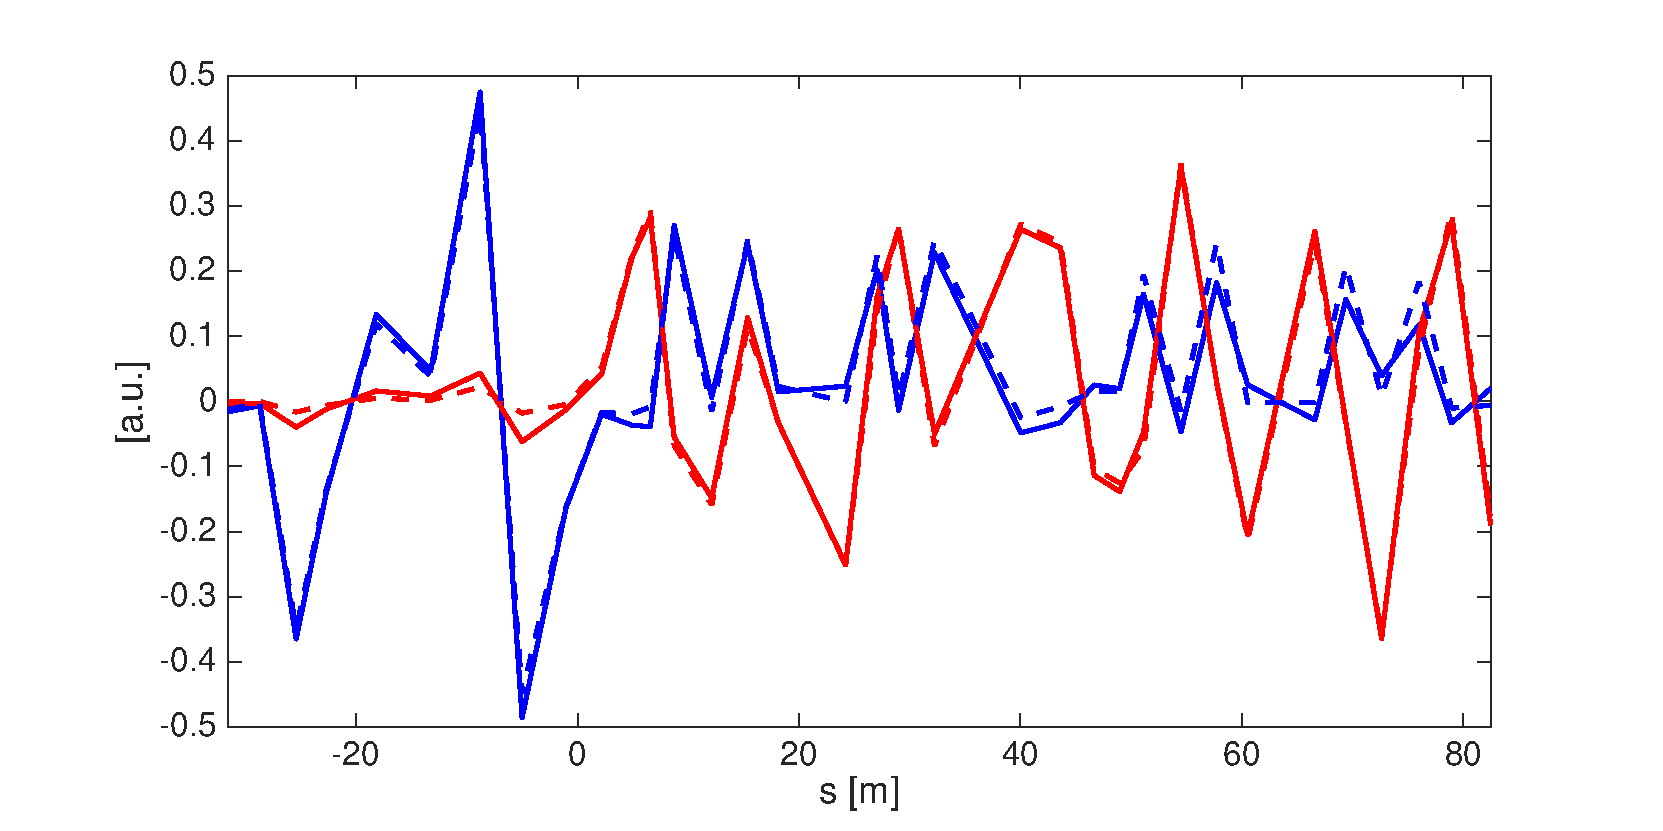
\includegraphics[width=0.66\textwidth]{obtainedSingularDirectionsV3.eps}
\label{fig:septaJitterAnalysisResponses}
}
\\%\qquad
\subfloat[]{
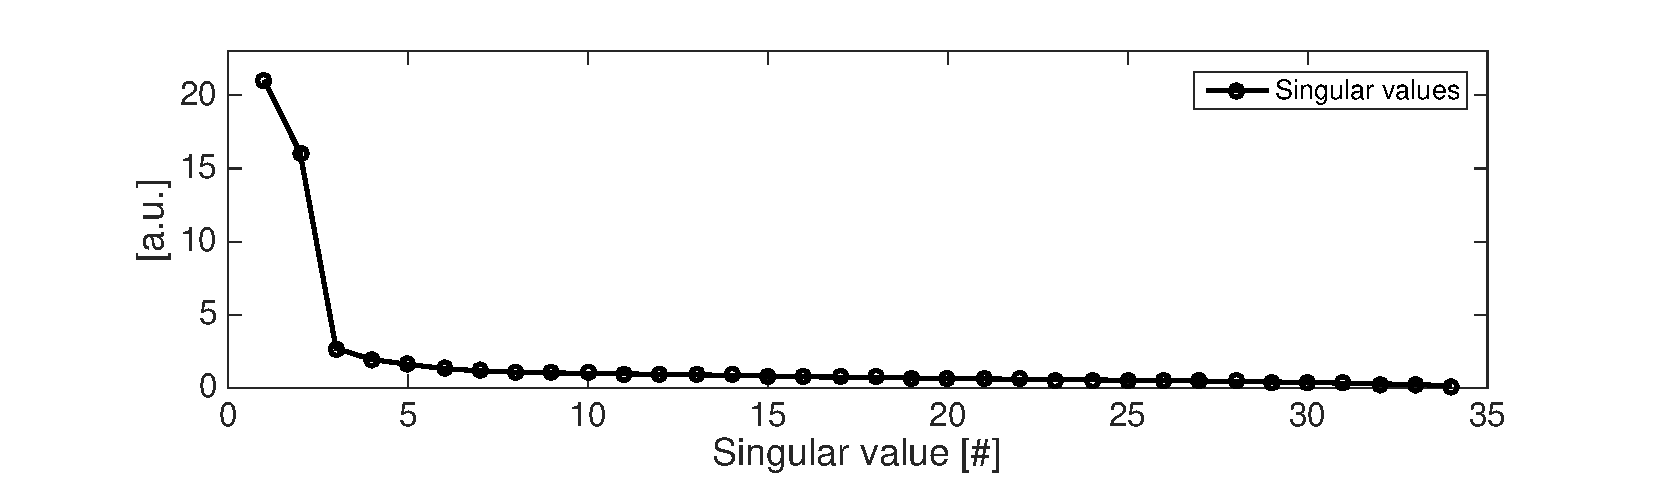
\includegraphics[width=0.66\textwidth]{genericSVDspectrum.eps}
\label{fig:septaJitterAnalysisSpectrum}
}
\caption{Example of jitter identification near the CR injection septa at CTF3.
%\protect\subref{fig:septaJitterAnalysisResponses} on the horizontal axis are the
different BPMs in that area.
\protect\subref{fig:septaJitterAnalysisResponses} on the horizontal axis is the position
of the available BPMs in the area with respect to the septa position ($s = 0$~m).
On the vertical axis is the normalised transverse orbit response under the effects of
septa variation (dashed-red line) and beam-energy variation (dashed-blue line).
The blue and red solid lines are the first and second singular directions of the SVD/PCA
analysis conducted on 100 consecutive beam orbits. 
\protect\subref{fig:septaJitterAnalysisSpectrum} the singular values spectrum of the
associated SVD decomposition.}
\label{fig:septaJitterAnalysis}
\end{figure}
%

It is clear that PCA can be a powerful method to measure and cross-check the dispersion
pattern,
as well as to identify other possible sources of orbit jitter.
This method has been implemented and successfully used in the dispersion monitor tool
developed at CTF3.


\subsubsection{Non-linear dispersion measurement}
%
In general one assumes that the beam orbit is linearly dependent on energy variations,
and practically this is most of the time a fair assumption.
Actually one should expect an inversely proportional dependence on the energy of the beam
(to some power), which is due to the kicks given to the beam from the magnetic elements
of the lattice (see~\cite{bib:DavideThesis}).
This means that for high energy variation and strong optics (like in CTF3) one might
expect non-linearities.
%
One might then wonder how the natural energy spread of the beam could interfere with the
measurement of the beam position,
and so with the dispersion measurement as a difference between two beam positions
readings.
If one assumes that the beam has a Gaussian energy distribution, then when the beam is
crossing a location affected by a generic non-linear dispersion the average beam position
is defined as:
%
\begin{align}
\langle x \rangle &=
\int_{-\infty}^\infty \mathrm{d}\frac{\Delta p}{p_0} \left[
D_x \frac{\Delta p}{p_0} +
DD_x \left(\frac{\Delta p}{p_0}\right)^2 +
DDD_x \left(\frac{\Delta p}{p_0}\right)^3 +
\cdots \right] \times \nonumber \\
&\qquad  \frac{1}{\sqrt{2\pi} \sigma_{\Delta p/p_0} } \exp \left( -\frac{1}{2} \left(\frac{\Delta p/p_0 - \langle \Delta p/p_0 \rangle}{\sigma_{\Delta p / p_0}} \right)^2 \right)
\label{eq:meanPosInNonLinDispStart}
\end{align}
%
where $D_x$, $DD_x$, ... are the linear and non-linear coefficients of the dispersion.
All integrals in Eq.~\ref{eq:meanPosInNonLinDispStart} are the non-central moments of the
Gaussian distribution.
This leads to:
%
\begin{align}
\langle x \rangle &=
D_x \langle \frac{\Delta p}{p_0} \rangle +
DD_x \left( \langle \frac{\Delta p}{p_0} \rangle^2 +  \sigma_{\Delta p / p_0}^2 \right) +
DDD_x \left( \langle \frac{\Delta p}{p_0} \rangle^3 +  3 \langle \frac{\Delta p}{p_0} \rangle \sigma_{\Delta p / p_0}^2
\right) +
\cdots
\label{eq:meanPosInNonLinDisp}
\end{align}
%
Equation~\ref{eq:meanPosInNonLinDisp} clearly shows that indeed the average beam position
is affected by the
beam-energy spread in the case of non-linear dispersion.
For the dispersion measurement one actually needs the orbit difference between two beams
with different energies, which
turns out to be:
%
\begin{align}
\Delta \langle x \rangle &=
D_x \Delta \langle \frac{\Delta p}{p_0} \rangle +
\left( DD_x + 3 DDD_x \sigma_{\Delta p / p_0}^2 \right) \Delta \left( \langle \frac{\Delta p}{p_0} \rangle^2 \right) +
\nonumber \\
&\qquad + \left( DDD_x + \cdots \right) \Delta \left( \langle \frac{\Delta p}{p_0} \rangle^3 \right) + \cdots
\label{eq:deltaPosInMultiOrderDispersion}
\end{align}
%
Similarly to the procedures described in Section~\ref{sub:detailDispMeas} one can then
collect a series of orbit differences under the effect of measurable energy variations,
and fit the \emph{linear} coefficients of 
Eq.~\ref{eq:deltaPosInMultiOrderDispersion} with respect to the \emph{powers} of the
energy variations and extract the linear dispersion coefficient $D_x$, which is $not$
affected by higher order dispersion and/or by the \emph{Gaussian} energy spread
$\sigma_{\Delta p / p_0}$.
Equation~\ref{eq:deltaPosInMultiOrderDispersion} highlights also other observations.
If for example the third order dispersion $DDD_x$ is negligible, then also the second
order dispersion is accessible with reasonable precision.
However the higher order the non-linear term, the more the energy spread of the beam might
affect the measurement.

At CTF3 the non-linear behaviour of the dispersion can be visible in areas with high
dynamic aperture, for example at the end of the linac after the Stretching Chicane.
Figure~\ref{fig:nonLinearitiesAfterFrascati}\subref{fig:nonLinearitiesAfterFrascatiMAD}
shows the expect non-linear dispersion at three BPMs after the Frascati chicane, which is
normally set with a strong optics ($R_{56} = 0$ optics).
The simulation is performed by considering a random displacement of the quadrupoles in the
line of the order of $100 \mu m$, which is the typical alignment precision of CTF3. 
Figure~\ref{fig:nonLinearitiesAfterFrascati}
\subref{fig:nonLinearitiesAfterFrascatiMeasure} shows a real measurement performed in
2014: the beam energy variation on the $x$ axis is computed from the horizontal beam
position at the first dispersive BPM in the Frascati chicane.
%
\begin{figure}[h]
\centering
\subfloat[]
 {
  \includegraphics[width=0.45\textwidth]{simulations.eps}
  \label{fig:nonLinearitiesAfterFrascatiMAD}
 }
\qquad
\subfloat[]
 {
   \includegraphics[width=0.45\textwidth]{measurements.eps}
   \label{fig:nonLinearitiesAfterFrascatiMeasure}
 }
\caption{Example of non-linear dispersion measurement at the end of the linac at CTF3.
         \protect\subref{fig:nonLinearitiesAfterFrascatiMAD} the MAD-X simulation of the single
         particle horizontal position as a function of the momentum error at three different BPMs
         installed in the area,
         and whose name is specified in the legend.
         \protect\subref{fig:nonLinearitiesAfterFrascatiMeasure} a measurement of the average beam
         momentum as a function of the beam-momentum error.
         The measurement has been performed at the same BPMs simulated in
         \protect\subref{fig:nonLinearitiesAfterFrascatiMAD}.
         For each BPM the total mean position has been subtracted.
}
\label{fig:nonLinearitiesAfterFrascati}
\end{figure}
%
Even though the two plots in Figure~\ref{fig:nonLinearitiesAfterFrascati} have different vertical axis scales,
the non-linear behaviour of the orbit dependence on the beam energy is extremely similar between measurement and simulation.
The factor 2 scaling difference between the two plots is not justified by the effect presented in Eq.~\ref{eq:deltaPosInMultiOrderDispersion},
but it could be attributed to calibration error of the BPMs, which was suspected but never verified. 
Still one can state that at CTF3 non-linear energy effects are present and at least qualitatively measurable.


\subsubsection{Application features}
%
The \emph{onlineDispersion} MATLAB application developed at CTF3 implements all the
measurements described in the previous sections. % \ref{sub:detailDispMeas}. 
The common ingredient for all these measurement is to collect a certain number of
consecutive orbits.
At each new beam shot a new orbit is collected, stored in a circular buffer of the desired
size, and the dispersion calculation is performed on the stored data and the Graphical
User Interface (GUI) is updated.
It turned out that the ``online'' approach adopted is very useful to obtain an immediate
feedback on the quality of the measurement even after only a few shots.
%
A full list of the application features implemented can be summarised as follows:
%
\begin{itemize}
\item
Measurement and history of the estimated energy error ($\Delta p_i/p_0$) as the beam
position at a reference (dispersive) BPM, normalised by the nominal dispersion expected at
that location.
\item
Ability to wiggle the beam current and/or a set of selected magnets with definable
amplitudes and steps.
\item
Fit of the dispersion as the linear (or non-linear) correlation of each BPM's data with
respect to: 
the energy as measured at the reference BPM,
or the beam current as measured at the exit of the Drive Beam injector,
or the scaling of the specified magnets.
\item
PCA analysis of the acquired orbits and the singular value spectrum is always visible on
the application GUI.
\item
Detailed view of a generic SVD analysis (Eq.~\ref{eq:svdDecompositionOfOrbitsGeneric}) of
the acquired orbits, including the display of the weighted singular directions in the
orbit space (columns of matrix $\mathbf{U}$) and time space (columns of matrix
$\mathbf{V}$).
\item
Detailed view, by scatter plot, of the correlation between a selected BPM and either the
reference BPM or the magnet scaling or the beam current scaling.
\item
Measurement and history of the ``dispersive'' component of the mean beam orbit.
This is computed simply by operating the scalar product between the measured dispersion
and the mean orbit as measured by the BPMs.
A dispersive component different from zero might be a sign that the optics is not matched
to the mean energy of the beam.
\end{itemize}
%
The main graphical interface of the application is illustrated in
Figure~\ref{fig:onlineDispersionGUI}.
The final implementation consists of a MATLAB compiled executable that loads a
user-editable XML\footnote{eXtensible Markup Language.} configuration file.
In this way the same application can be used to measure the dispersion in any desired
beamline of CTF3.
The XML configuration file contains mainly the list of BPMs to monitor and the list of
magnets to use for the magnet-scaling measurement type.
All the details of the implementation and possible options and setup of the application
are beyond the scope of the present work.
It is worth mentioning that a separate GUI, not shown here, can display the detailed SVD
analysis of the acquired orbits.
This last GUI turned out to be extremely useful when more than one outstanding singular
value is detected: 
by looking at the detected singular direction in the observable space one has some hints
on the source of additional orbit jitter that is not correlated to the beam energy
variation. 

%%%%%%%%%%%%%%%%%
%
\begin{sidewaysfigure}
\centering
\begin{tikzpicture}
    \node[anchor=south west,inner sep=0] (image) at (0,0) 
    {\includegraphics[width=0.55\textwidth]{newDispInterface.png}};
    \begin{scope}[x={(image.south east)},y={(image.north west)}]
    %
        % main traces
        \draw[orange,ultra thick,rounded corners, fill=red!20, fill opacity=0.3]
         (0.01,0.302) rectangle (0.99, 0.77);
        \draw[orange,ultra thick,->] (0.99,0.55) -- (1.03,0.55) node [right, black,
         align=left, text width=5cm] 
        {Main view with all the acquired jitter traces and dispersion fits. On the $x$
        axis are the BPM names, on the $y$ axis the approximate dispersion. \\ 
        The jitter traces are in arbitrary units and scaled to fit the measured dispersion
        amplitude.};
        % bottom right
        \draw[orange,ultra thick,rounded corners, fill=red!20, fill opacity=0.3]
        (0.505,0.01) rectangle (0.99, 0.298);
        \draw[orange,ultra thick,->] (0.99,0.15) -- (1.03,0.15) node [right, black,
        align=left, text width=5cm] 
        {Jitter at the selected BPM and linear fit versus the chosen parameter: either
        beam current variation, or magnet scaling, or \emph{jitter at reference BPM}.};
        % bottom left
        \draw[orange,ultra thick,rounded corners, fill=red!20, fill opacity=0.3]
        (0.01,0.01) rectangle (0.495, 0.298);
        \draw[orange,ultra thick,->] (0.01,0.15) -- (-0.03,0.15) node [left, black,
        align=right, text width=5cm] 
        {Advance analysis: either \emph{singular values spectrum}, or history of the mean
        energy variations at reference BPM, or history of nominal dispersion component of
        the mean orbit.};
        %\draw[green!70!red, thick,->] (0.8,0.4) -- (0.7,0.3); % to indicate selected bpm
        % title of middle plot
        \draw[orange,ultra thick,rounded corners, fill=red!20, fill opacity=0.3]
        (0.25,0.77) rectangle (0.76, 0.81);
        \draw[orange,ultra thick,->] (0.25,0.795) -- (-0.03,0.6) node [left, black,
        align=right, text width=5cm] 
        {Number of shots collected and standard deviation of the observed energy
        jitter assuming nominal dispersion at the reference BPM.};
        \draw[orange,ultra thick,rounded corners, fill=red!20, fill opacity=0.3]
        (0.01,0.82) rectangle (0.55, 0.97);
        \draw[orange,ultra thick,->] (0.01,0.88) -- (-0.03,0.88) node [left, black,
        align=right, text width=5cm] 
        {Main control for the application and access to advanced menu for fine tuning of
        parameters and detailed analysis.};
        % top right controls
        \draw[orange,ultra thick,rounded corners, fill=red!20, fill opacity=0.3]
        (0.57,0.82) rectangle (0.99, 0.93);
        \draw[orange,ultra thick,->] (0.99,0.88) -- (1.03,0.88) node [right, black,
        align=left, text width=5cm] 
        {Specification of buffer size and main assumption on dispersion at the selected
        reference BPM.};
    %
    \end{scope}
\end{tikzpicture}
\caption{Online dispersion monitor. Main graphical interface.}
\label{fig:onlineDispersionGUI}
\end{sidewaysfigure}
%
%%%%%%%%%%%%%%%%%







% > \tb{Taken from Davide's LINAC16 paper}
% > 
% > The dispersion in a transfer line can be measured by 
% > changing the momentum of the beam with respect to 
% > the nominal momentum ($p_0$) the line is tuned for, 
% > and then measuring the mean orbit deviation.
% > %
% > The observed orbit displacement ($\Delta x$) can be expressed as:
% > %
% > \begin{align}
% > \Delta x = D_x \frac{\Delta p}{p_0} +
% >  DD_x  \left(\frac{\Delta p}{p_0}\right)^2 + 
% >  o\left(\left(\frac{\Delta p}{p_0}\right)^3\right).
% > \label{eq:simpleDispersionDefinition}
% > \end{align}
% > %
% > One can then fit the coefficients $D_x$, which is the linear dispersion, 
% > and if necessary also the higher order terms (e.g. $DD_x$).
% > Practically the measurement of $D_x$ is often sufficient to 
% > spot errors or mismatches in a beam line.
% > 
% > %
% > In transfer lines where dispersion is expected by design another 
% > interesting observable is what we call the ``nominal'' linear dispersion,
% > i.e. the orbit response while scaling \emph{only} the bending magnets. 
% > This quantity is not affected by quadrupole misalignments and orbit errors,
% > hence it is a direct measurement, with opposite sign, 
% > of $D_x$ in Eq.~\ref{eq:simpleDispersionDefinition} for the ideally aligned 
% > linear machine \cite{bib:DavideThesis}.
% > Note that the measured quantity is \emph{not} the actual dispersion 
% > experienced by the beam,
% > but it is the dispersion contribution of the bending magnets which, 
% > in an ideal-linear machine, are the only sources of dispersion.
% > This observable turns out to be useful for optics verification and 
% > it can be used to define the target dispersion for DTS.
% > 
% > %
% > At CTF3 a MATLAB application to perform online measurements of 
% > linear and non-linear dispersion has been developed \cite{bib:DavideThesis}.
% > The relative energy of the beam with respect to the beam lines can be 
% > varied mainly in three ways:
% > %
% > \begin{itemize}
% > \item
% > By scaling all the magnetic elements in the line. Note that this method 
% > would not reveal the \emph{incoming} dispersion, 
% > but only the dispersion generated within the section of beam line being scaled.
% > \item
% > By scaling the beam current delivered by the thermionic gun. 
% > Since the Drive Beam linac relies on fully loaded accelerating structures, 
% > one can assume a linear correlation between beam current and 
% > beam acceleration \cite{bib:CTF3DesignReport}.
% > \item
% > By varying the phase and/or power of the accelerating structures in the linac, 
% > which has a similar effect as scaling the beam current.
% > \end{itemize}
% > %
% > The more convenient method is to vary the beam current. 
% > 

\subsection{Quadrupole Scans}
\label{03_2_QuadScans}
\tb{Taken from Davide's IPAC17 paper MOPAB115}
%Davides IPAC17 2017  MOPAB115

Quadrupolar Scan technique was employed to measure emittance and Twiss parameters with help of 
a profile monitors~\ref{01_MTV}.
It is one of the main methods routinely employed in 
relativistic beams in transfer lines, and it is extensively documented in the literature 
(e.g. in~\cite{Lohl2005}).
Here we recall only the basic principles for the simplest case of a
linear and uncoupled transfer line,
where one can treat the horizontal and vertical phase-spaces
independently using a 2D matrix formalism.
%
%For 4D reconstruction of the transverse phase space one can see, for example, ~\cite{}.
A quadrupole scan consists in reconstructing the transverse phase-space
distribution at some location along a beam line by measuring the beam
profile downstream.
In linear optics the transfer matrix from a \emph{reconstruction} (R)
to a \emph{measurement} (M) location can be written as:
%
\begin{align}
\begin{pmatrix}
x \\
x'
\end{pmatrix}_M
&=
\begin{bmatrix}
A & B \\
C & D
\end{bmatrix}
\begin{pmatrix}
x \\
x'
\end{pmatrix}_R
\label{eq:simpleTranport}
\end{align}
where $A$, $B$, $C$, $D$ are coefficients that depends on the layout of
the beam line and on the strength of its quadrupoles. 
%
The beam variance ($\sigma_M^2$) at the measurement location can be
expressed as a function of the Twiss parameters $\alpha_R$, $\beta_R$
and $\gamma_R$ at the reconstruction location as:
%
\begin{align}
 \sigma_M^2 = \beta_M \epsilon &= 
 \begin{pmatrix}
  A^2 & -2AB & B^2 
  \end{pmatrix} 
\begin{pmatrix}
   \beta_R \\
   \alpha_R \\
   \gamma_R
\end{pmatrix}
\epsilon
\label{eq:varianceForQuadscan}
\end{align}
%
where $\epsilon$ is the beam \emph{geometric} emittance.
Further we will use the \emph{normalised}
emittance definition $\epsilon_N = \epsilon \, \gamma_{\text{rel}}$
where $\gamma_{\text{rel}}$ is the relativistic factor. 
\todo[inline]{\textepsilon for geometric or normalized?}
\tr{Piotr: I think it will be easier to leave \textepsilon~ for normalized and define here $\epsilon_G$ for geometric.
Otherwise in all the plots and tables we need to stick N next to epsilon.}
%
One can measure the beam variance $\sigma_{M,i}^2$ (e.g. with an
intercepting screen as normally done at CTF3)
while varying the strength of the quadrupoles and therefore the
coefficients of the transfer matrix, 
and so solve linear system of equations:
%
\begin{align}
\begin{pmatrix}
\sigma_{M,1}^2 \\
\sigma_{M,2}^2 \\
\vdots \\
\sigma_{M,n}^2
\end{pmatrix}
&=
\begin{pmatrix}
\beta_{M,1} \\
\beta_{M,2} \\
\vdots \\
\beta_{M,n}
\end{pmatrix}
\epsilon 
= 
 \begin{pmatrix}
  A_1^2 & -2A_1B_1 & B_1^2 \\
  A_2^2 & -2A_2B_2 & B_2^2 \\
  \vdots & \vdots & \vdots \\
  A_n^2 & -2A_nB_n & B_n^2 \\
  \end{pmatrix} 
\begin{pmatrix}
  \beta_R \\
  \alpha_R \\
  \gamma_R
\end{pmatrix}
\epsilon.
\label{eq:dataCollectionQuadscan}
\end{align}
%
Finally by knowing that the Twiss parameters must satisfy the relation
$\beta\gamma - \alpha^2 = 1$, one can disentangle and obtain both the
beam emittance and the Twiss parameters at the reconstruction location.

%%%%%%%%%%%%%%%%%%%%%%%%%%%%%%%%%%%%%%%%%%%%%%%%%%%%%%%%%%%%%%%%%%%%%%%%%%%%%%%%%%%%%%%%%%%%%%%%%%%%%
%%%%%%%%%%%%%%%%%%%%%%%%%%%%%%%%%%%%%%%%%%%%%%%%%%%%%%%%%%%%%%%%%%%%%%%%%%%%%%%%%%%%%%%%%%%%%%%%%%%%%
%%%%%%%%%%%%%%%%%%%%%%%%%%%%%%%%%%%%%%%%%%%%%%%%%%%%%%%%%%%%%%%%%%%%%%%%%%%%%%%%%%%%%%%%%%%%%%%%%%%%%

\subsubsection{Constant beam size}

The necessary condition for obtaining a good fit is that the matrix in
Eq.~\ref{eq:dataCollectionQuadscan} is well conditioned. 
A standard way is to vary a single quadrupole strength such that the
beam size at the measurement location goes through a minimum. 
However this is not necessary, and sometimes one might want to keep the
beam size constant or within a certain range due to limitations of the
measurement device (e.g. poor resolution or field of view of the screen
used).
This was already exploited at the former CLIC Test Facility 2 (CTF2) in
\cite{Tenenbaum1997} and used elsewhere, e.g. in \cite{prat2014}.
Here one needs an initial estimate of the Twiss parameters that are
going to be measured, and so build a well conditioned matrix of the
coefficients in Eq.~\ref{eq:dataCollectionQuadscan} according to the
given constraint.

At CTF3 we use the MATLAB \emph{fsolve} solver \cite{mat:solver} for
setting up such a measurement.
Figure~\ref{fig:constantBeam} shows a comparison of two measurement
performed on the Drive Beam at CTF3.
The first one, in blue, has been obtained by varying only one
quadrupole, while three quadrupoles have been used for the measurement
in red.
The second measurement, using the Twiss parameters measured from the
first one, was set up trying to keep the beam size constant at the
screen.
The fitted Twiss parameters are reported in
Table~\ref{tab:constantBeam}.
%
\begin{figure}[htb]
   \centering
   \includegraphics*[width=0.6\columnwidth]{MOPAB115f3.eps}
   \caption{Horizontal beam variance $\sigma_{xx}$ measured at the screen for different settings of quadrupole settings. Dashed are the expected values from the fitted Twiss parameters.}
   \label{fig:constantBeam}
\end{figure}
%
%
\begin{table}[bt]
   \centering
   \begin{tabular}{ l c c c c c}
    \hline                
                & $\beta_x$ [m]      & $\alpha_x$          & $\epsilon_{Nx}$ [$\mu$mm] \\
  %Normal       & $5.02\pm0.19$      & $-3.53\pm0.14$      & $155\pm3$ \\
  %Constant     & $3.98\pm0.17$      & $-2.64\pm0.12$      & $146\pm3$ \\
  Standard      & $5.0\pm0.2$        & $-3.5\pm0.1$        & $155\pm3$ \\
  Constant size & $4.0\pm0.2$        & $-2.6\pm0.1$        & $146\pm3$ \\
    \hline
   \end{tabular}
   \caption{Twiss Parameters Fitted from the Measurements Shown in Fig.~\ref{fig:constantBeam}}
   \label{tab:constantBeam}
\end{table}
%
Note that the fitted Twiss parameters, while being not too far, are not
fully consistent.
This is believed to be due to the Gaussian fit that is applied to the
measured profiles, which sometimes can be far from being Gaussian as
shown later in Fig.~\ref{fig:tomo}~\protect\subref{fig:tomoprofiles}.
%%%% Could be added:
This provide also an idea of the accuracy of such a measurement. 
The experience at CTF3 is that when comparing the Twiss parameters of
two different beam setups it is good practice to use the same scan
settings. This allows to minimise the systematic errors when comparing
the obtained values.
%%%%
Probably due to a systematic error on the measurement which has not
been revealed yet. 
This inconsistency have been observed several times at this location
while using different quadrupole scan ranges.

%%%%%%%%%%%%%%%%%%%%%%%%%%%%%%%%%%%%%%%%%%%%%%%%%%%%%%%%%%%%%%%%%%%%%%%%%%%%%%%%%%%%%%%%%%%%%%%%%%%%%
%%%%%%%%%%%%%%%%%%%%%%%%%%%%%%%%%%%%%%%%%%%%%%%%%%%%%%%%%%%%%%%%%%%%%%%%%%%%%%%%%%%%%%%%%%%%%%%%%%%%%
%%%%%%%%%%%%%%%%%%%%%%%%%%%%%%%%%%%%%%%%%%%%%%%%%%%%%%%%%%%%%%%%%%%%%%%%%%%%%%%%%%%%%%%%%%%%%%%%%%%%%


\subsection{Transverse matching}
%
In an ideal machine the beam is passing through the centre of the quadrupoles, 
therefore the beam centroid should not move while performing a quadrupole scan.
In practice this is not always the case,
but the movement of the beam centroid at the measurement location ($x_{M,i}$) 
can be used to fit the centroid phase-space coordinates ($x_R, x'_R$) 
by inverting the following system of equations: 
\begin{equation}
\begin{pmatrix}
  x_{M,1} \\
  x_{M,2} \\
  \vdots \\
  x_{M,n} 
\end{pmatrix}
= 
 \begin{pmatrix}
  A_1 & B_1 \\
  A_2 & B_2 \\
  \vdots & \vdots \\
  A_n & B_n \\
  \end{pmatrix} 
\begin{pmatrix}
  x_R \\
  x'_R 
\end{pmatrix}.
\label{eq:dataCollectionCentroide}
\end{equation}
%
Moreover, starting from the Twiss parameters and assuming Gaussian beams, 
one can represent the beam phase-space distribution as an ellipse of equation:
%
\begin{align}
\epsilon_x &= \gamma_x \, x^2 + 2 \alpha_x \, x \, x' + \beta_x \, x'^2.
\end{align}
%

At CTF3 the first recombination takes place into the Delay Loop (DL): 
half of the beam is \emph{delayed}, while the other half \emph{bypass} the DL. 
Both are then recombined in the following transfer line. 
Figure~\ref{fig:DLClosure} shows the ellipse representation in phase-space of 
a typical well matched delayed beam, bypass beam and 
relative factor two combined beam measured at CTF3.
The measured Twiss parameters and centroid coordinate are reported in Table~\ref{tab:DLClosure}.
%
\begin{figure}[htb]
   \centering
   \includegraphics*[width=0.6\columnwidth]{MOPAB115f2.eps}
   \caption{Phase-space representation of a bypass (red), delayed (blue) and combined (green) beam 
            for an example measurement at CTS. 
            Dashed are the expected nominal ellipses assuming the measured emittances.}
   \label{fig:DLClosure}
\end{figure}
%
\begin{table*}[bt]
   \centering
   \caption{Beam Centroid and Twiss Parameters Related to Fig.~\ref{fig:DLClosure}}
   \begin{tabular}{ l c c c c c}
    \hline
    	&  $y$ [mm]	& $y'$ [mrad]	& $\beta_y$ [m]	& $\alpha_y$	& $\epsilon_{Ny}$ [$\mu$mm] \\
Bypass beam	& $-1.12\pm0.06$	&$ 0.03\pm0.01$	& $8.56\pm0.48$	& $-0.25\pm0.04$	& $142\pm4$ \\
Delayed beam	& $-1.24\pm0.06$  	&$-0.04\pm0.01$	& $7.17\pm0.53$	& $-0.43\pm0.05$	& $119\pm4$ \\
Combined beam	& $-1.21\pm0.06$   	&$ 0.04\pm0.01$	& $7.71\pm0.21$	& $-0.32\pm0.02$	& $152\pm2$ \\
    \hline
   \end{tabular}
   \label{tab:DLClosure}
\end{table*}
%

%%%%%%%%%%%%%%%%%%%%%%%%%%%%%%%%%%%%%%%%%%%%%%%%%%%%%%%%%%%%%%%%%%%%%%%%%%%%%%%%%%%%%%%%%%%%%%%%%%%%%
%%%%%%%%%%%%%%%%%%%%%%%%%%%%%%%%%%%%%%%%%%%%%%%%%%%%%%%%%%%%%%%%%%%%%%%%%%%%%%%%%%%%%%%%%%%%%%%%%%%%%
%%%%%%%%%%%%%%%%%%%%%%%%%%%%%%%%%%%%%%%%%%%%%%%%%%%%%%%%%%%%%%%%%%%%%%%%%%%%%%%%%%%%%%%%%%%%%%%%%%%%%


\subsubsection{Dispersion effect}
%
One of the effects that can spoil the accuracy of a quadrupole scan is the
presence of unwanted dispersion in conjunction with high beam energy spread.
%The effects of a large energy spread on the emittance measurement has been studied for the CLIC decelerator in \cite{Olvegard2013114}.
%Here we recall only the simplest linear dispersion effect.  Equation~\ref{eq:varianceForQuadscan} should be written as:
In the simplest case of a beam line without bending magnets and assuming
only linear dispersion, Eq.~\ref{eq:varianceForQuadscan} can be rewritten
as:
%
\begin{align}
 \sigma_M^2 &= 
 \beta_M \epsilon + D^2_{M} \sigma_p^2 \\
&=
 \begin{pmatrix}
  A^2 & -2AB & B^2 
  \end{pmatrix} 
\begin{pmatrix}
   \beta_0 \epsilon + \sigma_p^2 D_{R}^2 \\
   \alpha_0 \epsilon - \sigma_p^2 D_{R} D^{\prime}_{R} \\
   \gamma_0 \epsilon + \sigma_p^2 D_{R}^{\prime\,2} 
\end{pmatrix}
\label{eq:varianceForQuadscanWithDisp}
\end{align}
%
%
where $D$ and $D'$ are the dispersion coordinates, while $\sigma_p$ is the
beam r.m.s. energy spread. 
%The dispersion at the screen, $D_{x, s}$, is the propagation of the incoming %dispersion, $D_{x,0}$, and its derivative with respect to $s$, $D_{p_x,0}$,
%that propagate under the effect of the same coefficients $A$ and $B$.
%$\sigma_p$ is the r.m.s. energy spread that here is assumed to be normally
%distributed.
Note that from Eq.~\ref{eq:varianceForQuadscanWithDisp} there is no way with a
simple quadrupole scan to disentangle the additional dispersion contribution
from the ``betatronic'' one.
On the other hand the presence of dispersion makes the beam centroid position
change if the beam energy is varied. 
Each equation of the system in Eq.~\ref{eq:dataCollectionCentroide} can then
be rewritten as:
%
\begin{align}
x_M
&=
\begin{bmatrix}
A & B
\end{bmatrix}
\begin{pmatrix}
x_R + D_{x,R} \, \Delta p/p_0 \\
x'_R  + D'_{x,R} \, \Delta p/p_0
\end{pmatrix}_R
\label{eq:simpleTranportPlusDisp}
\end{align}
%
where the $D_{x,R}$ and $D'_{x,R}$ are the dispersion coordinates at the
reconstruction location and $\Delta p/p_0$ the applied relative beam energy
variation.
During a quadrupole scan on can vary the beam energy as well, and collect all
beam centroid positions.
From this data one can fit the initial centroid coordinates and dispersion
inverting Eq.~\ref{eq:simpleTranportPlusDisp}, and use this information to
subtract the dispersion contribution from
Eq.~\ref{eq:varianceForQuadscanWithDisp}.

Figure~\ref{fig:dispersionFit} shows an example of such a measurement
performed at CTF3.
%
\begin{figure}[htb]
   \centering
   \includegraphics*[width=0.6\columnwidth]{MOPAB115f1.eps}
   \caption{Horizontal beam position $x$ measured at a screen as a function of quadrupole current $I_Q$. The colour code is the beam energy variation with respect to nominal.}
   \label{fig:dispersionFit}
\end{figure}
%
From this data we could fit an incoming dispersion of  $D_x = -141 \pm 16$~mm
and $D'_x = -16 \pm 1$~mrad.
On the quadrupole scan data, by including this contribution the measured beam
emittance goes from $\epsilon_x = 171\pm5$ to $128\pm17$, i.e. a reduction of
about 25\%.


%%%%%%%%%%%%%%%%%%%%%%%%%%%%%%%%%%%%%%%%%%%%%%%%%%%%%%%%%%%%%%%%%%%%%%%%%%%%%%%%%%%%%%%%%%%%%%%%%%%%%
%%%%%%%%%%%%%%%%%%%%%%%%%%%%%%%%%%%%%%%%%%%%%%%%%%%%%%%%%%%%%%%%%%%%%%%%%%%%%%%%%%%%%%%%%%%%%%%%%%%%%
%%%%%%%%%%%%%%%%%%%%%%%%%%%%%%%%%%%%%%%%%%%%%%%%%%%%%%%%%%%%%%%%%%%%%%%%%%%%%%%%%%%%%%%%%%%%%%%%%%%%%

\subsubsection{Other Limiting factors}


Comment on uncertainty and repeatability of the measurements and their sources
\begin{itemize}
\item Screen calibration
\item The fitting
\item The local model
\item The machine stability
\end{itemize}


Troubles finding range

Large alpha 

%%%%%%%%%%%%%%%%%%%%%%%%%%%%%%%%%%%%%%%%%%%%%%%%%%%%%%%%%%%%%%%%%%%%%%%%%%%%%%%%%%%%%%%%%%%%%%%%%%%%%
%%%%%%%%%%%%%%%%%%%%%%%%%%%%%%%%%%%%%%%%%%%%%%%%%%%%%%%%%%%%%%%%%%%%%%%%%%%%%%%%%%%%%%%%%%%%%%%%%%%%%
%%%%%%%%%%%%%%%%%%%%%%%%%%%%%%%%%%%%%%%%%%%%%%%%%%%%%%%%%%%%%%%%%%%%%%%%%%%%%%%%%%%%%%%%%%%%%%%%%%%%%

\subsection{Transverse phase-space tomography}
%
\todo[inline]{We should put some tomographt results and conclusions or remove this section}
The idea of applying tomographic techniques for phase space reconstruction
has been introduced in \cite{McKee1995} and extensively studied in the
literature, e.g. in \cite{Lohl2005, Hock2011}.
The concept is to use the whole beam profile measured, and not only the
fitted beam variance. 
The mathematical background is well explained with the help of
Fig.~\ref{fig:tomoPhaseSpaces} from \cite{Hock2011}.
%
\begin{figure}
\centering
\subfloat[]{ %[reconstruction location]
%%%%%%%%%%%
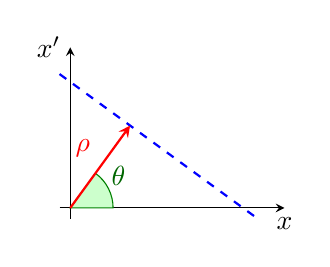
\begin{tikzpicture}[ 
    scale			= 0.68,
    %axis/.style		= {help lines, -{Stealth[length = 1.5ex]}},
    >=stealth
  ]
% axes
\draw[->] (-0.2,0) -- (4,0) node [below] {$x$};
\draw[->] (0,-0.2) -- (0,3) node [left] {$x'$};
% tilted line
\draw[-,blue, dashed, thick] (-0.2,2.5) -- (3.5,-0.2);
% angle
\filldraw[fill=green!20,draw=green!50!black] (0,0) -- (0.8,0) arc [start angle=0, end angle=54, radius=0.8] -- cycle;
% pointing arrow
\draw[->,red, thick] (0,0) -- node[above left]{$\rho$} (54:1.9);
% add some labels
\node[green!40!black] at (0.9,0.6) {$\theta$};
%
\end{tikzpicture}
\label{fig:tomoPhaseSpaceInitial}
%%%%%%%%%%%
}
% Start of second figure with circles
\,
%
\subfloat[]{ %[screen location]
%%%%%%%%%%%
\begin{tikzpicture}[ 
    scale			= 0.68,
    %axis/.style		= {help lines, -{Stealth[length = 1.5ex]}},
    >=stealth
  ]
% axes
\draw[->] (-0.2,0) -- (4,0) node [below] {$x$};
\draw[->] (0,-0.2) -- (0,3) node [left] {$x'$};
% tilted line
\draw[-,blue, dashed, thick] (2.5,-0.2) -- (2.5,3);
% pointing arrow
\draw[->,red, thick] (0,0) -- node[above]{$\rho'$} (0:2.5);
%
\end{tikzpicture}
\label{fig:tomoPhaseSpaceScreen}
}
\caption{
Correspondence between a phase-space profile integral line (dashed line) at the reconstruction location~\protect\subref{fig:tomoPhaseSpaceInitial} and at the measurement location~\protect\subref{fig:tomoPhaseSpaceScreen}.
The red arrows identify the distance of the integral line from the origin of the axes at the two locations.
}
\label{fig:tomoPhaseSpaces}
\end{figure}
%
Each point of a measured beam profile can be seen as a line integral over the
vertical-dashed line in
Fig.~\ref{fig:tomoPhaseSpaces}~\protect\subref{fig:tomoPhaseSpaceScreen}.
This is equal to the integral along the dashed line in
Fig.~\ref{fig:tomoPhaseSpaces}~\protect\subref{fig:tomoPhaseSpaceInitial}
representing the phase space at the reconstruction location. 
Assuming the linear transformation in Eq.~\ref{eq:simpleTranport}, the angle
$\theta$ and the relation between the distances $\rho$ and $\rho^{\prime}$
can be found to be:
%
\begin{align}
 \tan(\theta) &= \frac{B}{A} \qquad
 \rho' = \rho \sqrt{A^2 + B^2}.
\label{eq:tomographyRelations}
\end{align}
In practice each measured profile is a compressed projected distribution of
the beam phase space taken at different angles.
By carefully decompressing the profiles one can therefore use them for
reconstructing the actual beam phase-space distribution.
At CTF3 this is done by using the inverse Radon transformation provided by
MATLAB \cite{mat:radon}. 

Figure~\ref{fig:tomo} shows a typical measurement performed at CTF3 with an
heavily non-Gaussian beam.
%
%  using data file eh7365894873.dat
% angles moving from about 50 to about 170 deg.
\begin{figure}[htb]
   \centering
   \subfloat[]{ %[screen location]
   	\includegraphics*[width=0.49\columnwidth]{MOPAB115f4.eps}
   	\label{fig:tomoprofiles}
   } \\
   \subfloat[]{ %[screen location]
   	\includegraphics*[width=0.49\columnwidth]{MOPAB115f5.eps}
   	\label{fig:tomorec}
   }
   \caption{Measured horizontal beam profiles~\protect\subref{fig:tomoprofiles} used for the transverse
            phase-space tomographic reconstruction in~\protect\subref{fig:tomorec}.
            Dashed is the phase-space reconstruction using the simpler quadrupole
            scan technique.}
   \label{fig:tomo}
\end{figure}
%
Note the non-Gaussian profiles measured at the screen location 
in~\ref{fig:tomo}~\protect\subref{fig:tomoprofiles}, 
which are well exploited by the tomographic reconstruction but 
obviously ignored by the simple quadrupole scan reconstruction. 


\subsection{Orbit Response Matrix}

The initial optics checks were done using Orbit Response Matrix method, where each
orbit corrector magnet is powered to observe the downstream orbit response. 
This way transfer matrix coefficient $R_{12}$ between the corrector magnet and 
the downstram BPMs is directly measured and can be compared
with the model values.

For each orbit measurement at least 5 consecutive shots were acquired, usually 7 or 10.
In a simple case the amplitude of the corrector excitations was the same for all devices
and was chosen to be the largest not provoking any important beam losses.
In order to maximize accuracy, in more sophisticated variant of the method, the excitation was
gradually increased for each corrector until the beam was fully transported over
4-5 downstream BPMs. For each BPM the measured offsets were plotted in function of 
the corrsponding corrector excitation currents and 
fitted in the range where no beam loss at given BPM was observed.
The tool was implemented in a MatLab script that 
fully automatized the measurement. 
The main results are listed in Section~\ref{sec:03_ModelImprovs}



\subsection{Phase Space Painting}

Phase space painting is a more sophisticated version of the Orbit Response Matrix method. 
The orbit is changed using a pair of consecutive orbit correctors such that 
position and momentum coordinates of the beam behind the second corrector follow a given ellipse. 
Normally it corresponds to the nominal Twiss parameters at this location or 
to values measured with a quad scan. 
Using these ones maximizes the chances that the beam stays within aperture all along 
the machine as the maximum orbit deviations should follow the nominal $\beta$-function pattern. 
Of course, assuming there is no large optics error. 
Another big advantage is that in this case the reconstructed phase advance can be 
directly compared with the model one. 

This method allows to measure directly phase advance in between BPMs 
independently of their calibration accuracy.  
$\beta$-function is also measured directly as a maximum observed orit amplitude, however, 
its accuracy depends on the BPM calibration.

Each measurement starts with defining 
\begin{enumerate}[nosep]
\item Names of the two corrector devices used to excite the beam
\item Their excitation constants
\item Beam energy $En$
\item Transfer matrix $R_{12}$ and $R_{22}$ components in between the correctors
\item Values of $\alpha$ and $\beta$ Twiss parameters to be painted
\item Area of the ellipse to be painted, i.e. the geometric emittance $\epsilon$
\item Plane (horizontal or vertical)
\item Number of points to paint $N_p$ 
\item Number of beam shots to be recorded for each orbit (usually between 5 and 10)
\end{enumerate}
A set of $\varphi_i$ angles is generated in range between $0$ and $\frac{3\pi}{2}$ 
in step of $\varphi_s = \frac{2\pi}{N_p}$.
Painting larger than $2\pi$ range provides more accurate fits, simply because it increases number of data points.
The spread of the points separated by $2\pi$ also gives a quick visual figure of stability of a particular measurement. 

The order of $\varphi_i$ angles is reshuffled such that 
$\varphi_{2i} - \varphi_{2i-1} = \pi$ and $\varphi_{2(i+1)} - \varphi_{2i} = \pi + \varphi_s$ to make the measurement 
less sensitive to any beam drifts. This reordering is illustrated in Fig.\ref{fig:PhSpEllipseConstr}. 
In this case differences of the consecutively measured orbits enter the analysis instead of 
differences with respect to the reference orbit (the one measured without any corrector magnet excitation). 
Alternatively, the reference orbit would have to be measured after every measurement point what would make 
the measurement twice longer. 

\begin{figure}[!h]
 \begin{center}
  \subfloat[]  %On the plot 16 Dec 2016 14:18
   {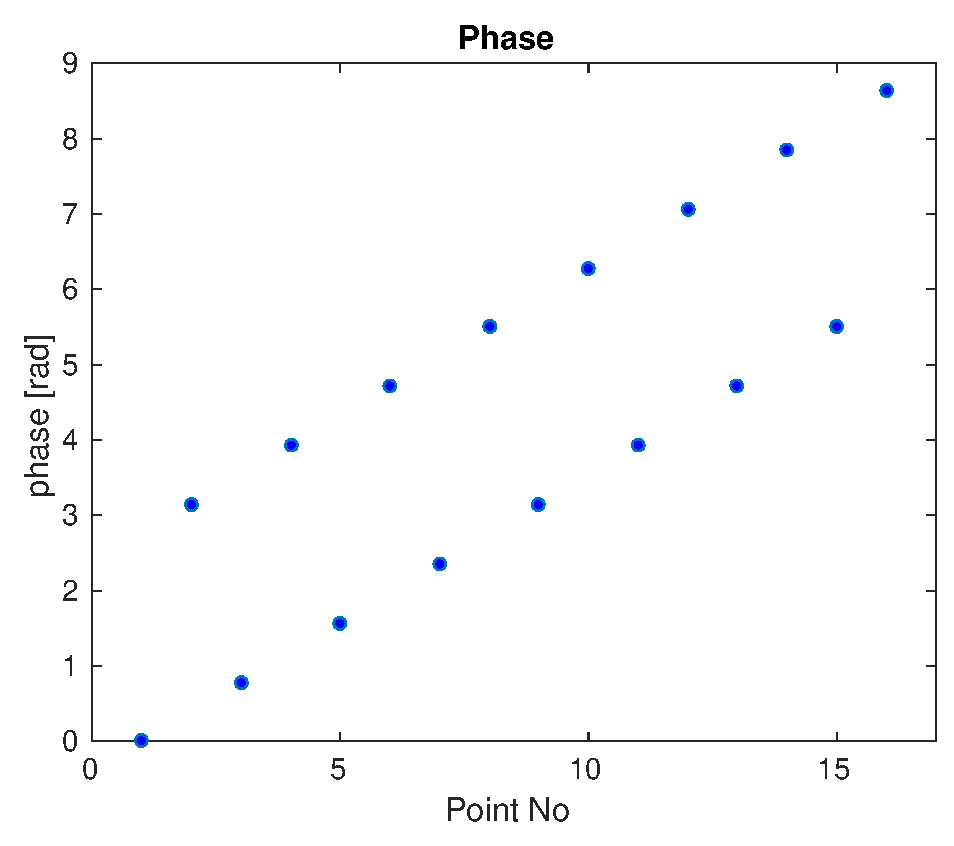
\includegraphics[width=0.45\columnwidth]{PaintedPhases.eps}} 
 \subfloat[]   %On the plot 15 Dec 2016 18:56
   {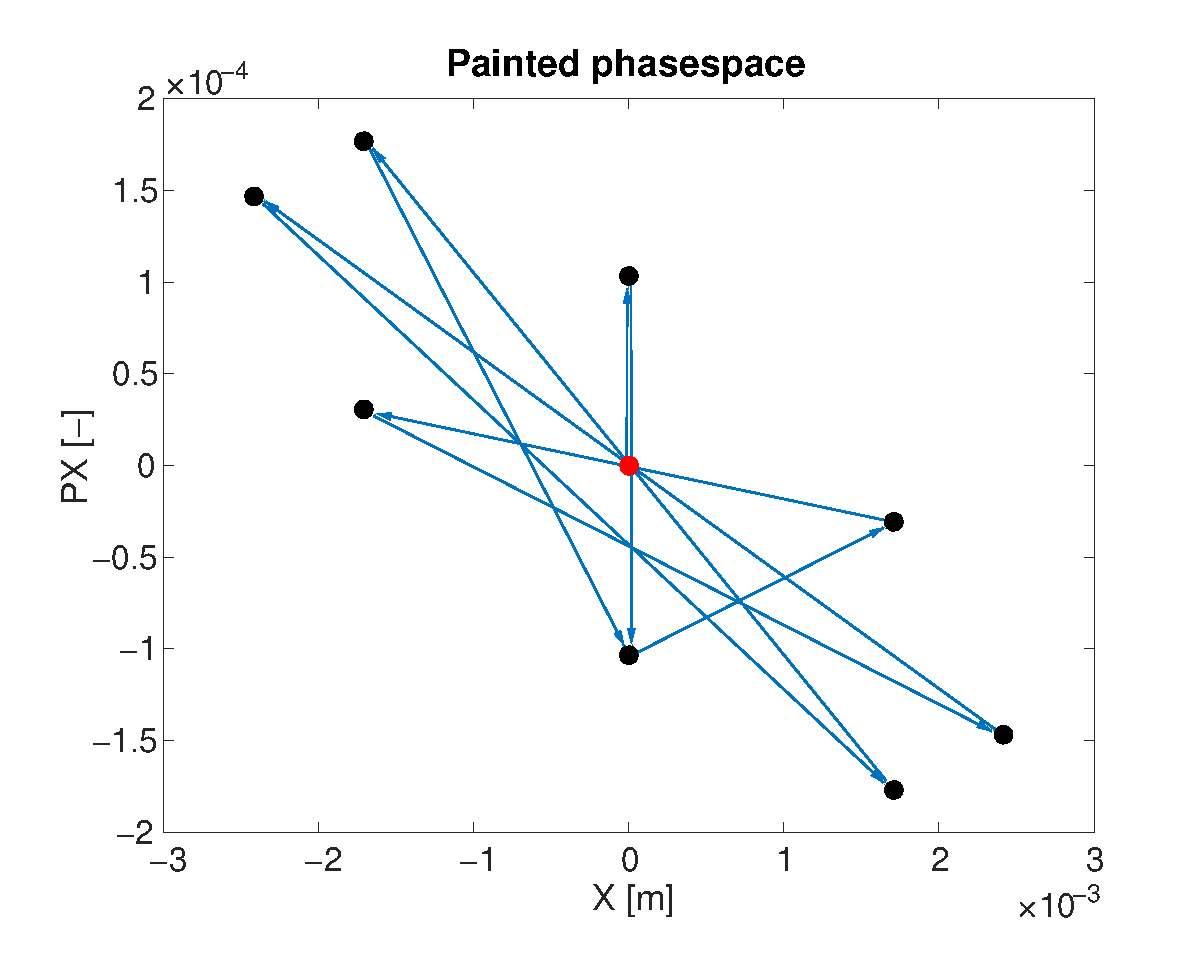
\includegraphics[width=0.51\columnwidth]{PaintedEllipse3.eps}}
 \end{center}
 \caption{Construction of the painted phase space ellipse.}
 \label{fig:PhSpEllipseConstr}
\end{figure}


A phase space ellipse with given $\alpha$, $\beta$ and $\epsilon$ has the following equation
\begin{align}
\begin{split}
   X_{i0}  &=  \sqrt{ \epsilon \beta } *cos(\varphi_i) \\
   XP_{i0} &=  \sqrt{ \frac{\epsilon } {\beta}} (-\alpha cos(\varphi_i)-sin(\varphi_i)) ,
\end{split}
\label{eq302_ellipseEq}
\end{align}
where  $\varphi_i$ is angle of $i_{th}$ point in the normalized coordinates. 
These are produced with the following kicks from orbit correctors 
\begin{align*}
   k_{1i} &=  X_{i0}/R_{12}, \\
   k_{2i} &=  XP_{i0} - k_{1i} \cdot R_{22},
\end{align*}
where $k_{1i}$ and $k_{2i}$ are angles due to upstream and downstream correctors, respectively, 
and $R_{12}$ and $R_{22}$ are components of the transfer matrix in between the two correctors. 
In order to minimize the model dependence of the measurement 
correctors separated only by a drift space were usually selected. 
In this case $R_{22}=1$ and $R_{12}=L_{12}$, where $L_{12}$ is distance in between the correctors. 
Finally, the excitation currents are computed using the particular magnet excitation constant and the beam energy.

Around 10 consecutive beam pulses were recorded for each painted point and 
their averages were used in the analysis. 
%In the first step the orbit differences between the consequtive points were calculated, from which 
Transverse coordinate $X$ was calculated as follows:
\begin{itemize}
 \item for the first point, the simple difference of the excited and the reference obrits, i.e. $X_1 = H_1 - H_0$,
       where $H_0$ and $H_1$ are the measured reference orbit (with no excitation) and the orbit for the first point
 \item for even points, half of difference between the orbit recorded for the given point and the previous one, 
       i.e. $X_{2i} = (H_{2i} - H_{2i-1}) / 2 $
 \item for the remaining odd points $X_{2i+1} = (H_{2i+1} - H_{2i}) - X_{2i}$
\end{itemize}

For each BPM a graph of $X$ in function of the painted phase was constructed.
A function of the form $A_{BPMn} \cdot sin(\varphi + \varphi_{BPMn})$ was fitted,
where $\varphi$ corresponds to abscissa and $A_{BPMn}$ and $\varphi_{BPMn}$ are the fit parameters.
$\varphi_{BPMn}$ measures phase advance between given BPM and the location where the
ellipse is painted, i.e. the downstream orbit corrector.
$A_{BPMn}$ measures size of the ellispe and if the BPM is well callibrated
\begin{equation}
\beta_{BPMn} = A^2_{BPMn}/\epsilon.
\label{eq:betaampl}
\end{equation}

Naturally, for the highest signal to noise ratio an ellipse with the largest area that 
can be transported without losses to the end of the section under study is searched.
In order to verify the procedure it was tested on a long drift line 
with multiple BPMs by depowering all the quadrupoles.
The observed discrepancy in phase advance allowed to correct the eventual errors in 
the excitations constants of the corrector magnets.

\begin{figure}[!h]
 \centering
  \subfloat[]  %On the plot 16 Dec 2016 14:18
   {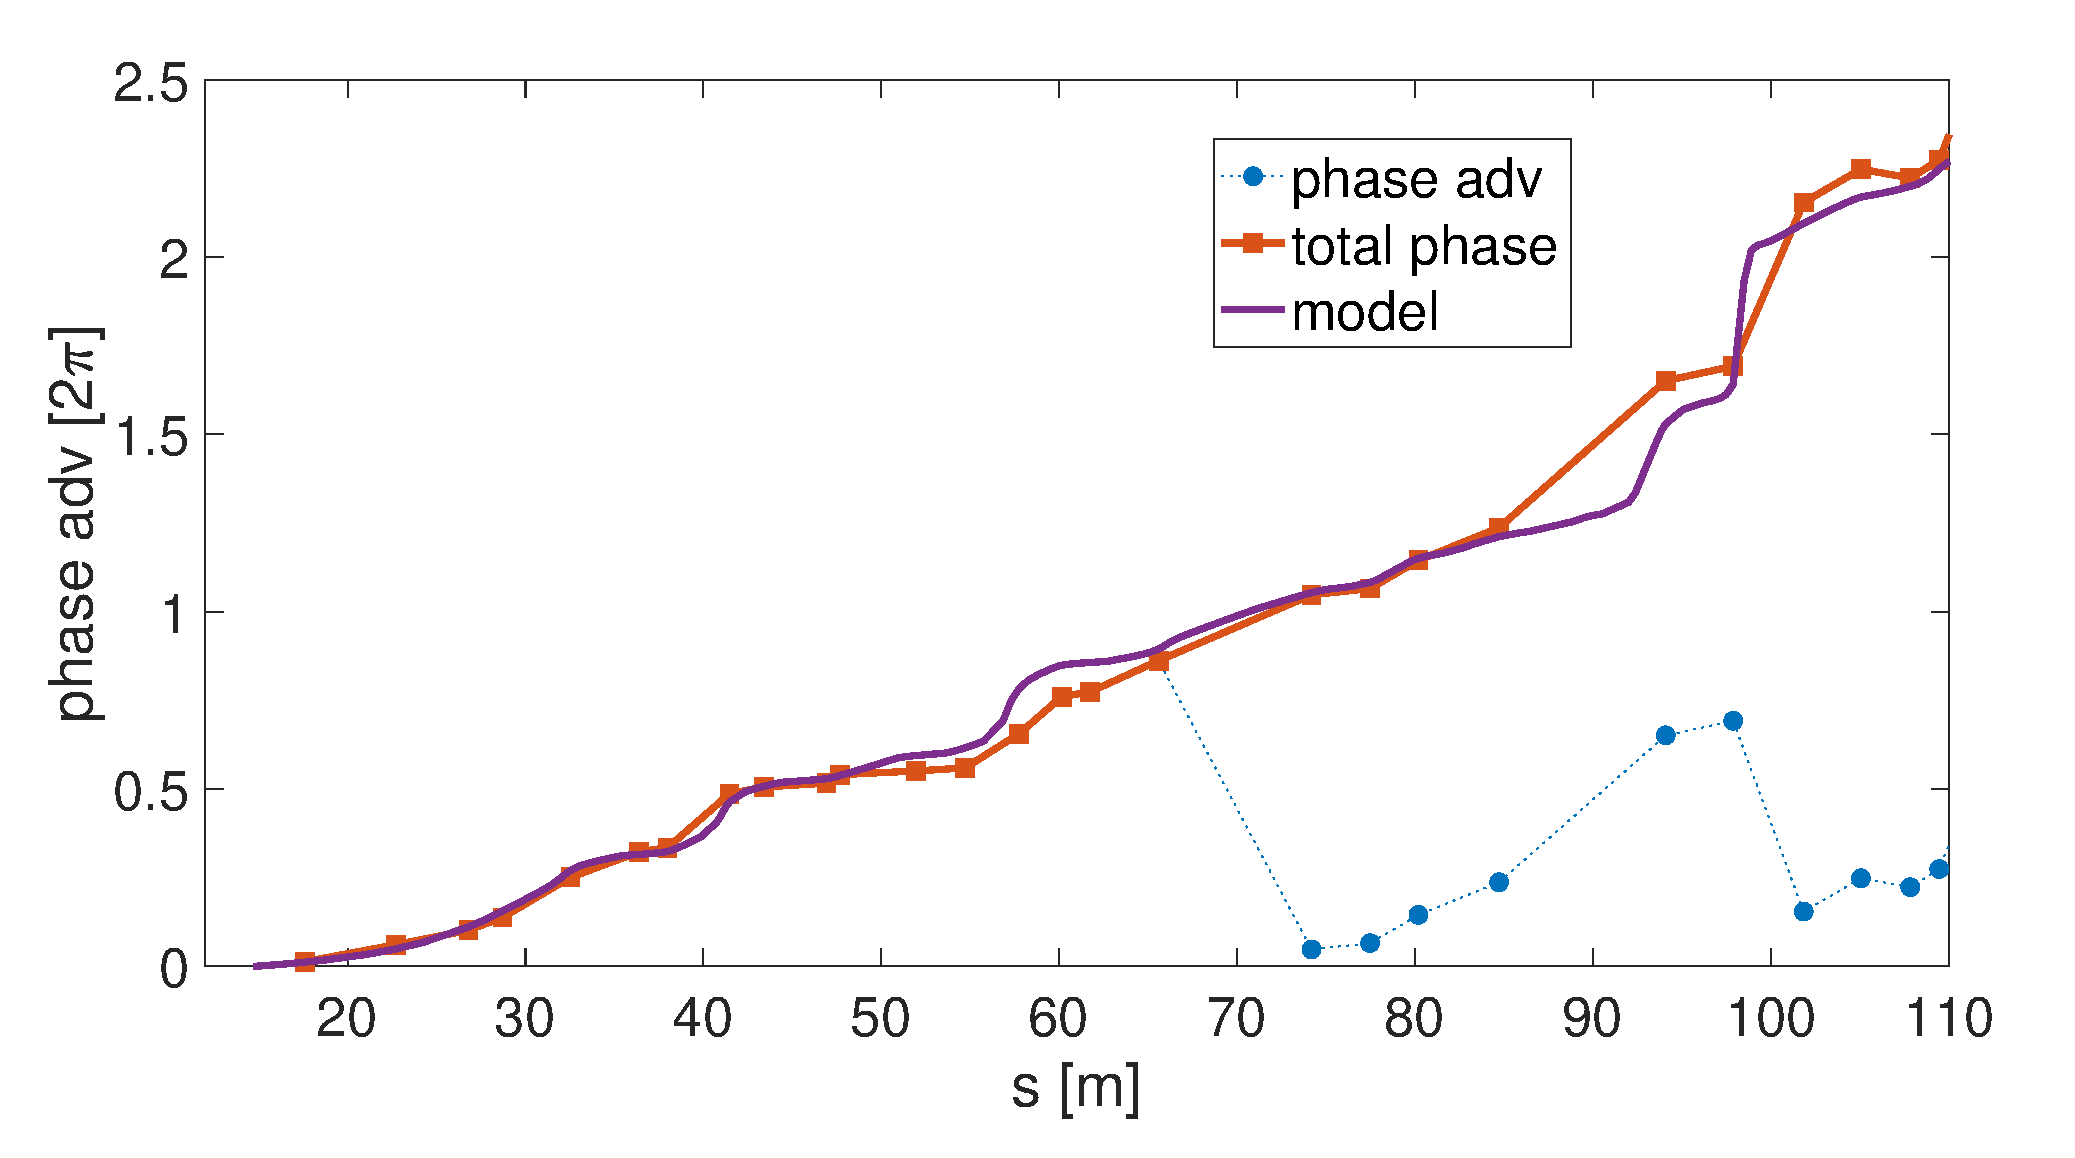
\includegraphics[width=0.49\columnwidth]{PhSPphase.eps}
    \label{fig:PhSPphase}} 
  \subfloat[]   %On the plot 15 Dec 2016 18:56
   {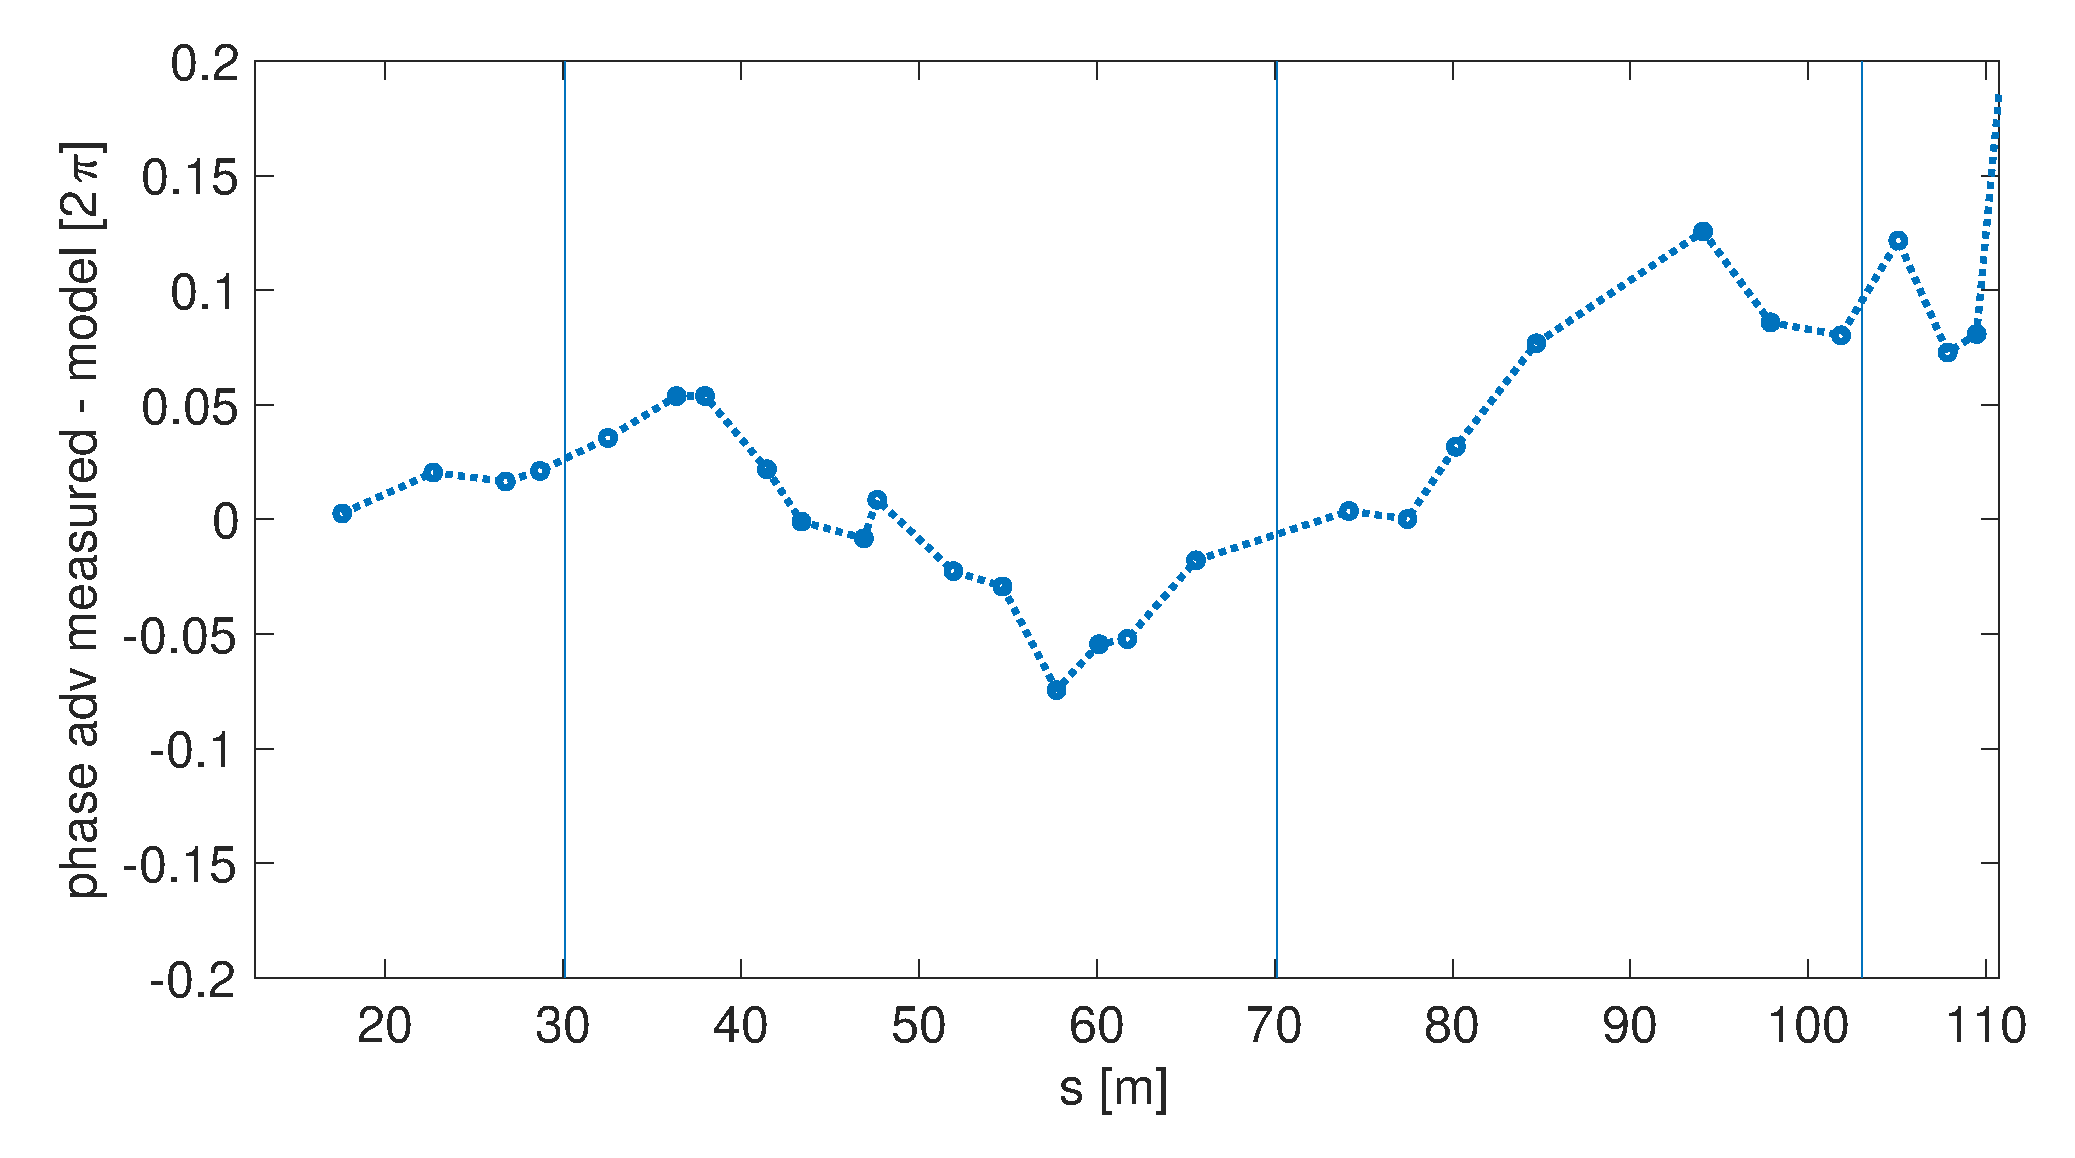
\includegraphics[width=0.49\columnwidth]{PhSPphase_diff.eps}
    \label{fig:PhSPphase_diff}}
 \caption{\protect\subref{fig:PhSPphase} Example of measured vertical phase advance and 
          \protect\subref{fig:PhSPphase_diff} its difference to the model.
          Vertical bars mark begining and end of the DL plus end of the TL1. }
 \label{fig:PhSpPhaseMeas}
\end{figure}


From phase differences between consequtive BPMs it was straight forward to obtain
the evolution of the phase advance along the machine, which was compared to the model
and eventually used for optics correction in conjunction with measured dispersion.
Figure~\ref{fig:PhSpPhaseMeas} presents an example measurement of CT line, DL and TL1
showing phase beating originating from the DL.

\textbeta -function was reconstructed using the 3-BPM method~\cite{bib:3BPMmethod}
\begin{equation}
\beta_{n} = \beta_{n~model}\frac{cot(\phi_{n-1}) + cot(\phi_{n+1}) }{cot(\phi_{n-1~model}) + cot(\phi_{n+1~model})}
\end{equation}
where $\phi_{n-1}$ is phase advance from the previous BPM and $\phi_{n+1}$ is to the following one.
This method assumes that the model transfer matrix between 2 consequtive BPMs is correct.
On the other hand, it not sensitive to BPM calibration errors.

The transfer matrix elements $R_{11}$ and $R_{12}$ between the location where the ellipse was painted
and given BPM were obtained by fitting function 
\begin{equation}
X_i = R_{11}X_{i0} + R_{12}*XP_{i0},
\label{eq:tm1}
\end{equation}
where $X_{i0}$ and $XP_{i0}$ are the painted coordinates defined by Equation~\ref{eq302_ellipseEq}.
Using Equation~\ref{eq:tm1} and the model values of the transfer matrix between consecutive
BPMs the momentum variable was reconstructed
\begin{equation}
XP_{n} = (X_{n+1} - X_{n})\frac{R_{11~model}}{R_{12~model}}.
\end{equation}
The reslting points were fitted with 
\begin{equation}
XP_i = R_{21}X_{i0} + R_{22}*XP_{i0},
\label{eq:tm2}
\end{equation}
allowing to find $R_{21}$ and $R_{22}$. Figure~\ref{fig:PhSpTM} illustrates an example measurement.

\begin{figure}[!h]
 \begin{center}
   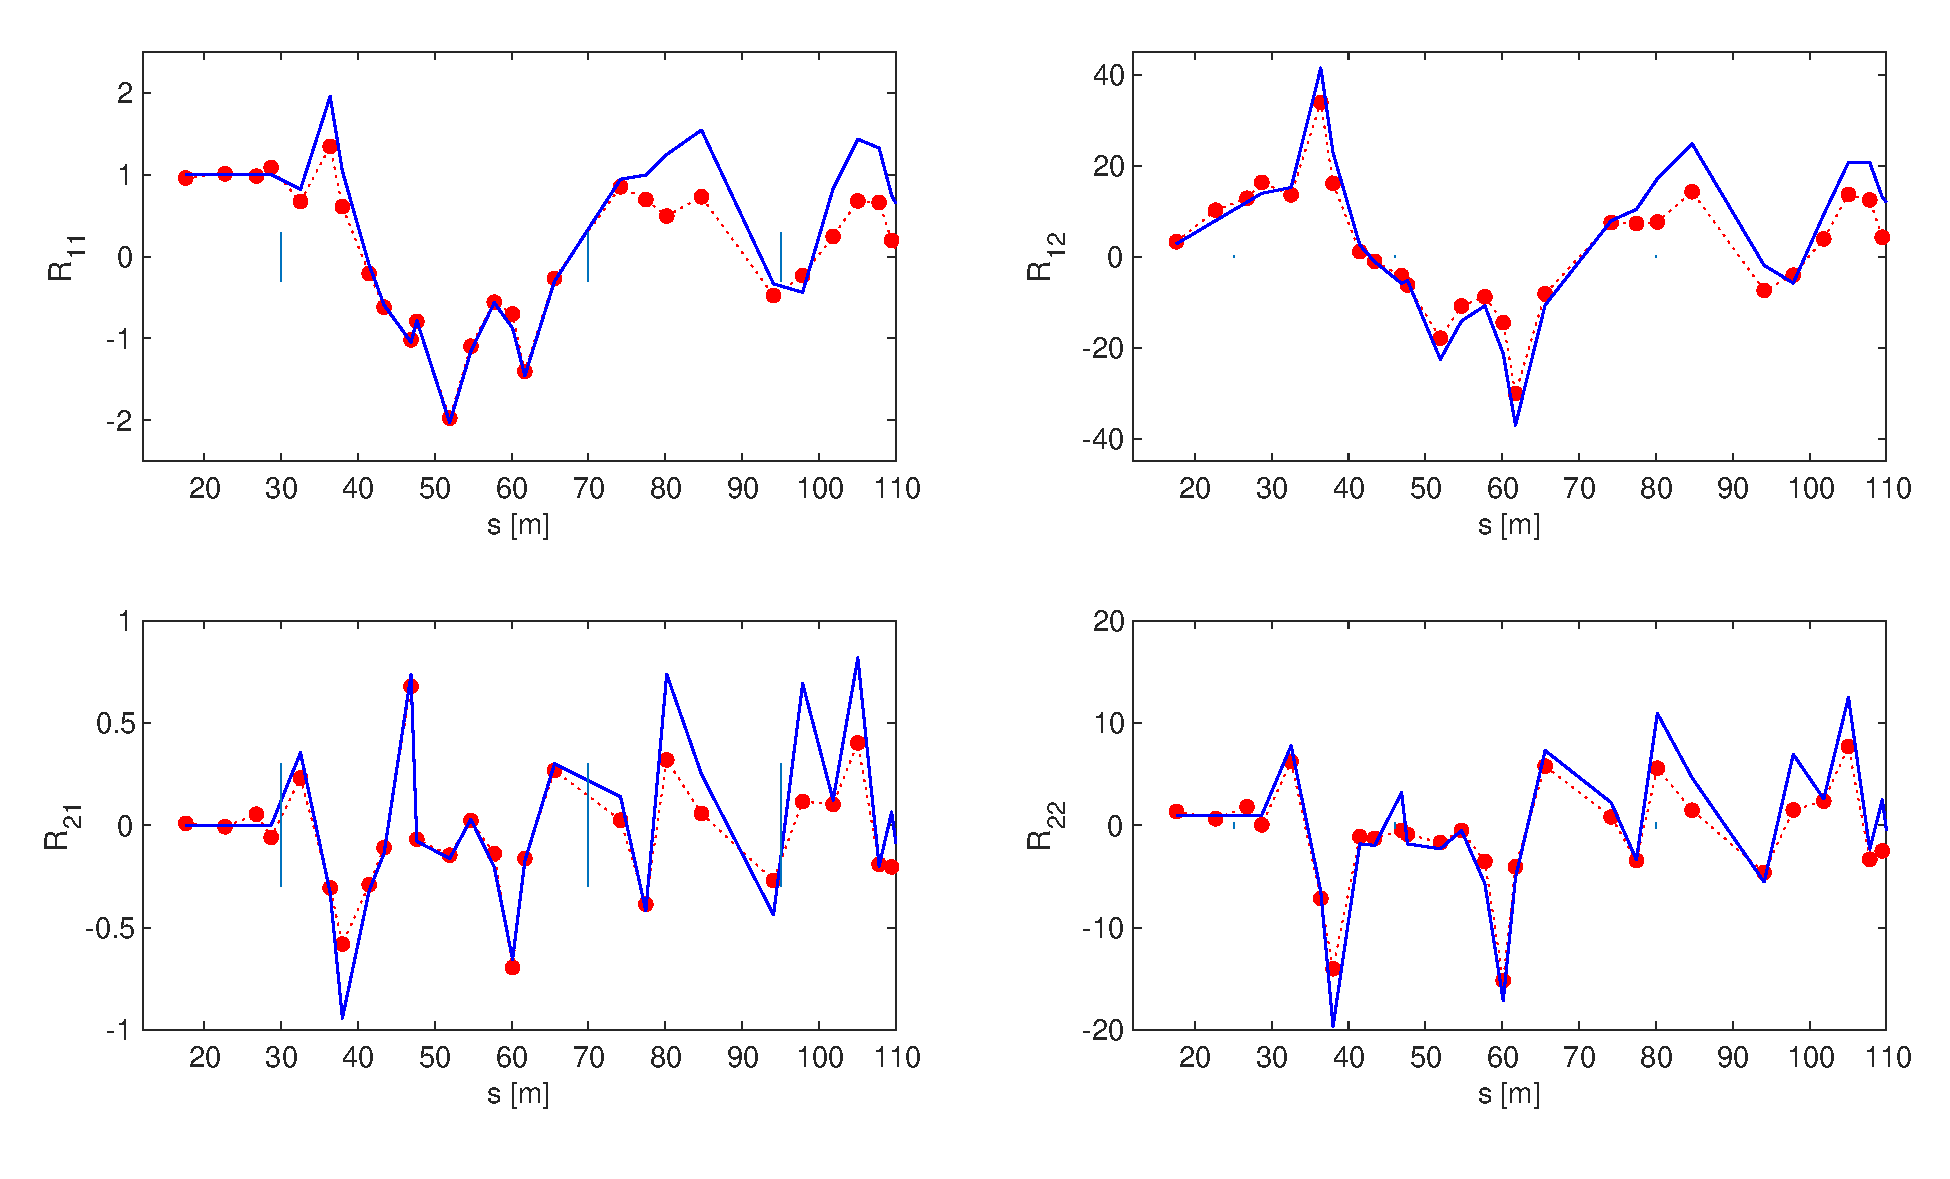
\includegraphics[width=0.99\columnwidth]{PhSPtm.eps} 
 \end{center}
 \caption{Example of measured vertical transfer matrix in 
          the CT, the DL and the TL1 illustrating an optics error.}
 \label{fig:PhSpTM}
\end{figure}


It was instructive to compare the obtained $X,XP$ with the model ellipse.
Ellipse equation was fitted yielding all Twiss parameters. 
Figure~\ref{fig:PhSpBeta} shows example of measured \textbeta -function 
using the described three methods in the CT, the DL and the TL1.

\begin{figure}[!h]
 \begin{center}
   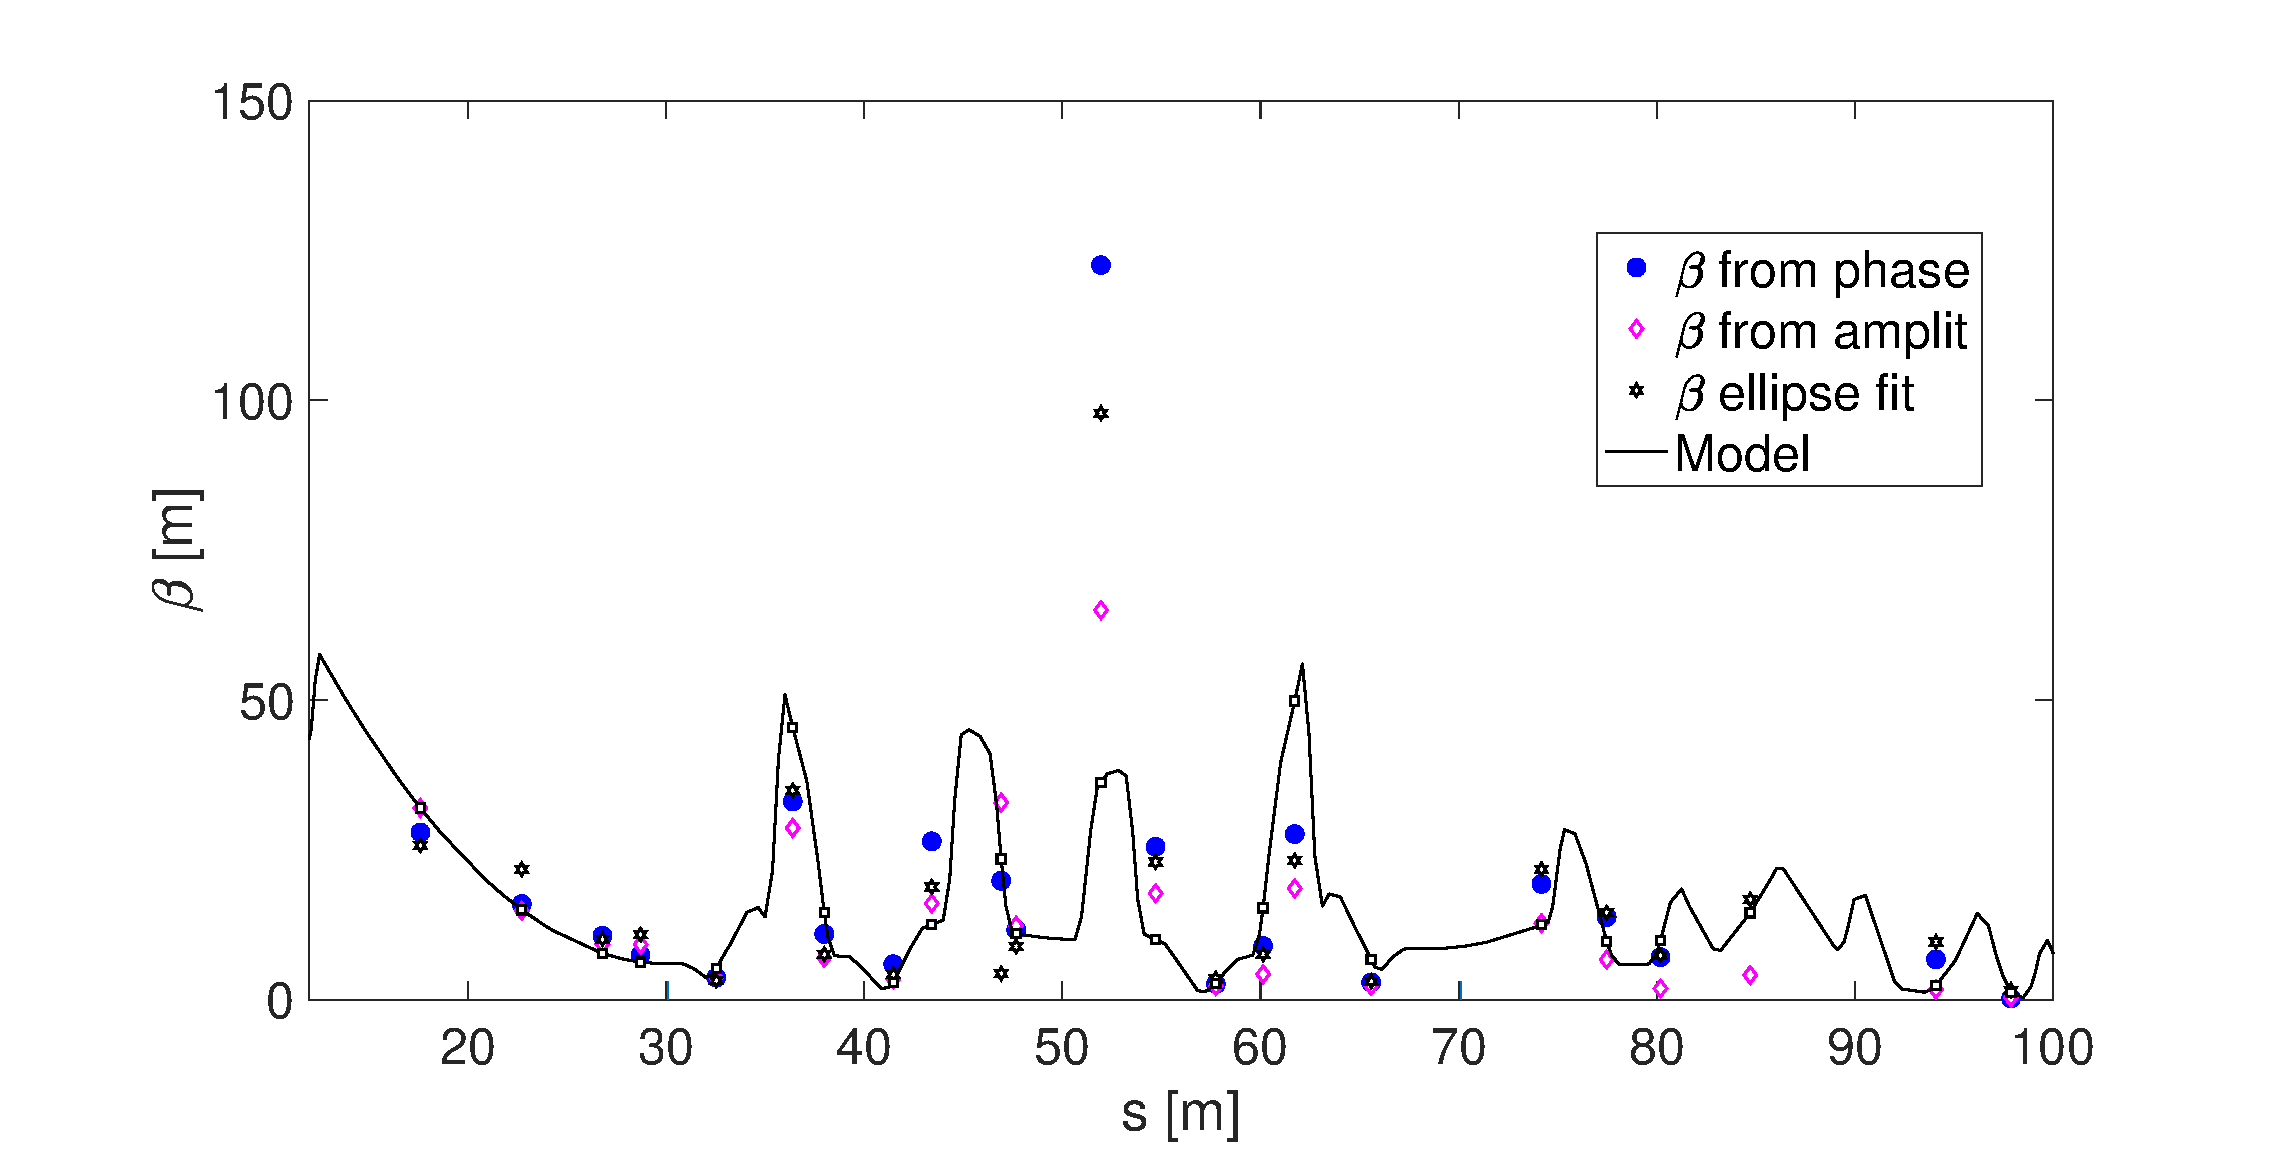
\includegraphics[width=0.75\columnwidth]{PhSPbeta.eps} 
 \end{center}
 \caption{Example of measured vertical \textbeta -function in the CT, the DL and the TL1.}
 \label{fig:PhSpBeta}
\end{figure}




 

\subsection{Tune measurements}

In the combiner ring the beam does a maximum of 4 turns. 
This makes the situation fundamentally different from a storage ring or 
synchrotron where particles make millions of turns so avoiding the integer or 
half integer resonances are not of the same importance. 
However, tune measurements can give detailed information about the optics and 
possible errors in the machine or in the model.

For the tune measurement the machine was set up for multi turn by shifting 
the timing of the extraction kicker to a later point in time. 
In order to measure the tune the beam was injected 
off the closed orbit into the combiner ring. 
The focusing strength of a quadrupole was changed to observe 
if the changes could be predicted by the model. 
The ideal situation would have been to change quadrupole by 
quadrupole and measure the change in tune.
However, in order to get an accurate tune measurement 
we can only tolerate small beam losses and 
this limits the amount of different settings that could be used.


To measure the tune the following steps have been done. 
They are described in detail in the forthcoming sections.
\begin{enumerate}
\item
Set up the combiner ring so the beam is circulating for at least 60 turns 
without losses.
\item
Acquisition of the signals from the BPMs with different settings of the magnets.
\item
Calculate the beam position for every BPM and every turn.
\item
Determine the average position over several pulses.
\item
Compensate for the charging-up effect.
\item
Fit each signal with a sinusoidal curve.
\item
If the fit is good enough, save the value and put it in the histogram with 
the other BPMs from the same measurement.
\item
Compare the values to the model.
\end{enumerate}


 
Figure~\ref{fig:bpm_not_charging_up} shows typical traces from a BPM directly read out 
from the control system. In the top the current trace is displayed, 
in the middle the horizontal position and in the bottom the vertical position. 
Every dip marks one turn in the combiner ring. 

Only the 12 first turns could be used due to strong dechoherence 
of the oscillation. The oscillation is damped to the closed orbit for the ring. 
Since the beam normally only does 4 turns in the combiner ring 
the closed orbit is not well-determined. 
\begin{figure}[!h]
\centering
%\includegraphics[scale=0.26,natwidth=1186,natheight=865]{fit_BPM8.png}
\includegraphics[scale=0.26]{fit_BPM8.png}
\caption{A sinusoidal fit over the position for different turns. \label{fig:fitOfPosition}}
\end{figure}
All fits were checked manually and if seen to fit the signal they were accepted and
placed as a count in a histogram. 
The histogram was then fitted with a Gaussian function and the mean and 
the $\sigma$ were saved for each measurement.
The fact that the tune or period of a sine is 
independent of amplitude of the oscillation makes the tune measurement 
independent of absolute calibration errors in the BPMs.
 
In order to determine if measure values are above or below 0.5, 
a quadrupole is changed by a few percent. 
Depending on if the quadrupole is focusing or 
defocusing in that plane and if the tune goes up or down it is possible to 
determine if the tune is above or below 0.5.  

All measurements that were made are summarised in Table~\ref{tab:tuneMeasureTime}. 
The number in the table corresponds to the number on the x-axis in 
Figure~\ref{fig:tuneModelVsMeasureHorizontal} and \ref{fig:tuneModelVsMeasureVertical}
\begin{table}[ht]
\centering
\begin{tabular}{| l | c | c |}
\hline
\textbf{number} & \textbf{time} & \textbf{change} \\ \hline
1 & 09:36:55 & 1\% down \\
2 & 09:34:30 & ref \\
3 & 10:01:31 & 0.5\% down \\
4 & 10:04:45 & 0.6\% down   \\
5 & 10:08:37 & 1.5\% down  \\
6 & 10:16:00 & 0.5\% down  CR.IQFF0510 up 1.5\% \\
7 & 10:27:20 & 0.5\% down  CR.IQFF0510 up 1.7\% \\
8 & 10:30:20 & 0.5\% down  CR.IQFF0510 down 6\% \\
9 & 10:35:00  & 0.5\% down  CR.IQDF0540 down 25\% \\
10 & 10:37:52 &  0.5\% down \\
11 & 10:43:48 &  0.5\% down  CR.IQDF0540 up 5\% \\
12 & 10:48:02 &  0.5\% down  CR.IQDH0340 down 11\% \\
13 & 10:50:05 &  0.5\% down  CR.IQDH0340 up 5\% \\
14 & 10:54:53 &  0.5\% down  quick test with sextupoles \\
\hline
\end{tabular}
\caption[Time and numbering of the tune measurement.]
{The column to the left corresponds to the x-label in 
figure \ref{fig:tuneModelVsMeasureHorizontal} and \ref{fig:tuneModelVsMeasureVertical}. 
The middle column is the time when the measurement was taken and 
the column to the right shows the change in the machine.  \label{tab:tuneMeasureTime}}
\end{table}
\begin{figure}[!h]
\centering
%\includegraphics[scale=0.30,natwidth=1253,natheight=719]{horizontal_tuneVsModel.png}
\includegraphics[scale=0.30]{horizontal_tuneVsModel.png}
\caption[Comparison between the tune from the model and the measurement in the horizontal plane]
{Comparison between the model, marked as *, 
and the measurement represented with the red error bars in the horizontal plane. 
\label{fig:tuneModelVsMeasureHorizontal}}
\end{figure}
 
The horizontal tunes for the different measurements series are presented in 
Figure~\ref{fig:tuneModelVsMeasureHorizontal}. 
The model's predictions are in most cases within the error bars 
but for some of the values they are slightly outside. 
Recalling that the error bars are only 1 $\sigma$ we expect 
3 out of 10 points to be outside the error bar, 
thus it is not possible to conclude that there is any error in the model. 
Nevertheless, it seems like the model slightly overestimates 
the change in tune when varying the focusing of a quadrupole.
 
\begin{figure}[!h]
\centering
%\includegraphics[scale=0.26,natwidth=1253,natheight=719]{vertical_tuneVsModel.png}
\includegraphics[scale=0.26]{vertical_tuneVsModel.png}
\caption[Comparison between the tune from the model and the measurement in the vertical plane]
{Comparison between the model, marked as *, and the measurement represented with 
the red error bars in the vertical plane \label{fig:tuneModelVsMeasureVertical}}
\end{figure}
In the case of the vertical tune, shown in figure \ref{fig:tuneModelVsMeasureVertical}. 
In this case three points are outside the error bar, which is close to the prediction. 
The fact that one of them is 2 $\sigma$ away is expected if we have 14 points.


The fit also provides information about the phase of each measurement. 
In this case the tune for the fit was fixed to a value obtained in the previous section 
while the tune phase were allowed to vary. 
The phase is aliased but by forcing the fit to be between $0 - \pi$ 
it is possible to compare the phases between different pickups. 
The difference in phase between two successive pickups were added together 
to get the overall phase advance. 
Figure \ref{fig:phaseAdvHorizontal} shows the phase advance for 
the horizontal plane while figure \ref{fig:phaseAdvVertical} shows it 
for the vertical plane. The error bar is 1 $\sigma$ and 
is calculated using the fitting environment in ROOT which takes the error bar into account
when calculating the uncertainty in each parameter.
 
\begin{figure}[!h]
\centering
%\includegraphics[scale=0.60,natwidth=932,natheight=589]{phaseAdvHorizontal.png}
\includegraphics[scale=0.60]{phaseAdvHorizontal.png}
\caption[Phase advance in the horizontal plane]
{Comparison between the model, marked as *, 
and the measurement represented with the green error bars in the horizontal plane. 
The black line shows the absolute difference between the measurement 
and the model. \label{fig:phaseAdvHorizontal}}
\end{figure}
 
\begin{figure}[!h]
\centering
%\includegraphics[scale=0.60,natwidth=970,natheight=682]{phaseAdvVertical.png}
\includegraphics[scale=0.60]{phaseAdvVertical.png}
\caption[Phase advance in the vertical plane]{Comparison between the model, 
marked as *, and the measurement represented with the green error bars 
in the vertical plane. 
The black line shows the absolute difference between the measurement and 
the model.\label{fig:phaseAdvVertical}}
\end{figure}
 
The result is overall in agreement with the model. 
Although, the precision needed to establish if there is a discrepancy 
between the measurement and the model between two consecutive pickups was not achieved. 
However, it provides the additional information that we are close to the design tune. 
With a new optics which corrects for the natural chromaticity more turns will be available
for analysis and increase the precision of the measurements.
 
In order to make more precise measurements it is important 
to be able to have more turns before the oscillation particles dechoere. 
The dechohrence was found to be be mainly due to chromaticity. 
There are sextupoles installed in CTF3 but the achromatic optics is not yet commissioned.
The settings of the sextupoles were found empirically. 
The best result obtained for the vertical oscillation is shown in 
Figure~\ref{fig:tune:sextopole_vertical}. 
This shows that it is possible to use sextupoles to alleviate the effect. 
The fact that we were unable to find a setting to reduce 
the horizontal chromaticity is because the orbit is worse in that plan. 
However, the use of sextupoles introduces extra complexity, 
since the focusing is dependent on the beam position inside the sextupole, 
resulting in a change in tune. 
This effect can be controlled by making sure that the beam passes through the centre of 
the sextupole, if necessary, with the help of correctors \cite{Minty_Zimmermann_Book}. 
The result is in line with a simulation done by Pierre-Louis Pernet \cite{pierre:tune}.    
 
\begin{figure}[!h]
\centering
%\includegraphics[scale=0.45,natwidth=1188,natheight=867]{sextopole_vertical.png}
\includegraphics[scale=0.45]{sextopole_vertical.png}
\caption{Vertical oscillation with sextupoles switched on.  \label{fig:tune:sextopole_vertical}}
\end{figure}
 

The overall agreement between the tune measurements and 
the model indicates that there are no major errors in the model. 
In order to reach higher accuracy it is necessary to implement 
the achromatic optics to reduce the chromaticity.
 

\subsection{Decoherence in the Combiner Ring \textbf{Tobias}}

One of the targets for CTF3 is to demonstrate a combined beam with emittance
below \unit[150]{$\pi\mu$m} for both planes \cite{roberto_telavi_linac}.
There are several factors that can increase the emittance in the combiner
ring, such as uncontrolled dispersion, unmatched lattice and miss-steering
at injection. A study was launched in 2012 to understand where the observed
increase was originating from. It was found that injecting onto the closed
orbit of the combiner ring was of key importance to minimize the emittance
growth. The emittance increase is caused by the large energy spread of the
beam in combination with high chromaticity in the combiner ring. 
The effect of decoherence is shown in figure~\ref{fig:decoherence} and described in
section~\ref{sec:aboutdechorense}. In figure~\ref{fig:emittance_growth} the
standard deviation around the closed orbit for a short pulse circulating 4
turns is plotted against the horizontal emittance. I varied the magnitude of
the oscillations around the closed orbit by changing corrector magnets
before the injection. The standard deviation is measured using 5 BPMs, the
quoted standard deviation is the mean of these value. It was repeated with a
beam combined 4 times. As seen in figure~\ref{fig:emittance_growth} the
emittance for this beam is larger than for the uncombined beam. 
The reason is that the different turns have slightly different orbits and 
hence they are together occupying a larger part of the transverse space. 
The measurements of the uncombined beam show good agreement with simulations
\cite{clic_workshop_cern_emittance}. 

\begin{figure}[!h]
\begin{center}
%\includegraphics[height=8.4cm,natwidth=341,natheight=262]{emittance_growth.pdf}
\includegraphics[height=8.4cm]{emittance_growth.pdf}
\end{center}
\caption{The horizontal emittance as a function of amplitude of the oscillations around the closed orbit. }
\label{fig:emittance_growth}
\end{figure} 

After a careful setup of the injection and extraction to the combiner ring 
a Drive Beam emittance of \unit[150]{$\pi \mu$m} was achieved for a factor 4 combined beam. 
The result is presented in Paper~\cite{ipac_ctf3_2013} together with a summary of recent achievements in CTF3. 
\todo{There should be another one with roughly the same values I think from later..}

\subsection{Bunch Length}

Bunch length was measured either directly with streak cameras or 
by RF phase scans and observation of beam profile.
RF power levels produced by the PETS gave acces to the effective bunch form-factor,
wich was used to crosscheck the measurements. 

\subsubsection{Streak Camera Measurements }

Streak cameras measured either the emitted synchrotron light or 
transition radiation of an intercepted screens. 

\subsubsection{\label{sec:rfphasescans}RF phase scans}


To ease the discussion, Figure~\ref{fig:PhScans_RF} shows an ideal cos-like accelerating voltage 
on which a bunch is occupying some phase length $\delta \phi$.
%
\begin{figure}[h]
\centering
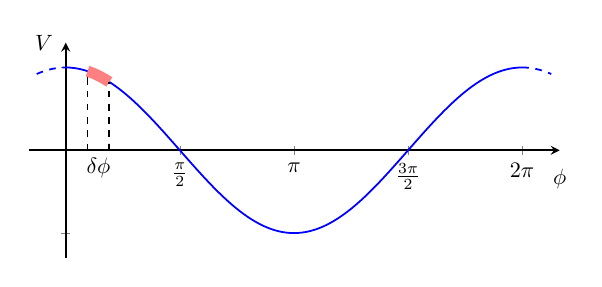
\begin{tikzpicture}[ 
    scale			= 0.8,
    %axis/.style		= {help lines, -{Stealth[length = 1.5ex]}},
    >=stealth
  ]
  \begin{axis}[
       thick,
       axis lines=middle,
       width = 10cm,
       height=5cm,
       xmin = -0.5,
       xmax = 6.8,
       ymin = -1.3,
       ymax = 1.3,
       xtick={0,1.5708,3.14159,4.7123889,6.283},
       xticklabels={$0$,$\frac{\pi}{2}$,$\pi$,$\frac{3\pi}{2}$, $2\pi$},
       yticklabel=\empty,
       x label style={at={(axis description cs:1,0.45)},anchor=north},
       y label style={at={(axis description cs:-0.005,1)},anchor=west},
       axis line style={->},
       xlabel=$\phi$,
       ylabel=$V$,
       domain=0:2*pi
       ]
    \addplot [samples=100,  thick, color=blue]{cos(deg(x))};
    \addplot [domain=-0.4:0, thick, color=blue, dashed]{cos(deg(x))};
    \addplot [domain=2*pi:(2*pi+0.4), thick, color=blue, dashed]{cos(deg(x))};
    \addplot [domain=0.3:0.6, line width=5pt, color=red!50]{cos(deg(x))};
    \addplot [thick, samples=50, smooth,domain=0:2,black, dashed] coordinates {(0.3,0)(0.3,{cos(deg(0.3))})};
    \addplot [thick, samples=50, smooth,domain=0:2,black, dashed] coordinates {(0.6,0)(0.6,{cos(deg(0.6))})};
    \node[below] at (axis cs:0.45, 0) {$\delta \phi$};
   % \legend{$\sin(x)$,$\cos(x)$,$x^2$}
    \end{axis}
\end{tikzpicture}
\caption{Accelerating voltage as a function of phase. In red is depicted a possible bunch of length $\delta \phi$ being accelerated.}
\label{fig:PhScans_RF}
\end{figure}
%
Assuming an ultra-relativistic beam, the beam energy ($E$) after going through 
a single accelerating structure can be written as:
%
\begin{align}
E &= E_0 + \Delta E_{max} \cos(\phi) 
\label{eq:EnergyGain}
\end{align}
%
where $E_0$ is the incoming beam energy; ($\phi = \phi_{RF} - \phi_{beam}$) is 
the phase of the RF ($\phi_{RF}$) with respect to the arrival phase of the beam 
($\phi_{beam}$); $\delta \phi$ is the length of the bunch in phase (see Fig.~\ref{fig:PhScans_RF}); 
$\Delta E_{max}$ is the maximum energy gain which is a constant that depends on 
the power delivered to the accelerating structure and the properties of the structure itself.

If the beam is off-crest in the accelerating structure one would expect, in very first approximation, 
a contribution to energy spread ($\Delta \delta E$) that depends on the bunch length $\delta \phi$ and 
phase $\phi$ equal to:
%
\begin{align}
\Delta \delta E &\approx \Delta E_{max} \sin(\phi) \delta \phi
\label{eq:energySpreadIncreaseBase}
\end{align}
%
In the limit case of $\phi = 0$ one gets maximum acceleration and, in first approximation, 
no energy spread variation.
In this case one might still want to estimate the impact on energy spread, 
which could be computed as:
%
\begin{align}
\Delta \delta E &= E_{max} \left(1-\cos\left(\frac{\delta \phi}{2}\right)\right).
\label{eq:energySpreadIncreaseOnCrest}
\end{align} 


%
The contribution from Eq.~(\ref{eq:energySpreadIncreaseBase}) should then be added in quadrature 
to the initial beam energy spread ($\delta E_0$).
%
In reality, the incoming beam might have some time-correlated energy spread, 
therefore a more precise estimation of the final beam energy spread is:
%
\begin{align}
\delta E &= \sqrt{
(\delta E_0)^2 + 
\left(
C
+
\Delta E_{max} \sin(\phi)
\right)^2  \delta\phi ^2
}
\label{eq:completeEnergySpreadVariation}
\end{align}
%
where $\delta E_0$ is the initial \emph{un-correlated} energy spread, 
$C$ is the incoming beam energy-spread-time correlation factor.

%
By doing a scan of $\phi_{RF}$ and by measuring the final energy $E$, 
from Eq.~(\ref{eq:EnergyGain}) one can fit $E_0$,  $\Delta E_{max}$ and beam phase $\phi_{beam}$.
%
At the same time, by rerecording also the beam energy spread variation, 
one can fit Eq.~(\ref{eq:completeEnergySpreadVariation}) unknown parameters: 
$\delta E_0$, $C$ and the sought $\delta\phi$.

Note that $\delta\phi$ is in units of $2 \pi$. The bunch length in seconds ($\delta\phi_{s}$) is 
linked to the RF frequency ($f_{RF}$) via:
%
\begin{align}
\delta\phi_{s} &= \frac{1}{f_{RF}} \frac{\delta\phi}{2 \pi}
\label{eq:conversionRadToS}
\end{align}
%

The above equations can be used only assuming Gaussian distributions, 
for which $\delta\phi$, $\delta E_0$, $\Delta \delta E$ can either be, consistently, 
the r.m.s. or FWHM values using the known relation:
\begin{align}
{\mathrm  {FWHM}}=2{\sqrt  {2\ln 2}}\;\sigma \approx 2.355\;\sigma.
\end{align}



% Assuming an ultra-relativistic electron beam, and dealing with only one accelerating structure, 
% one would expect that the acceleration and energy spread variation goes like:
% %
% \begin{align}
% \Delta E &= A \cos(\phi) \label{eq:energyIncreaseBase} \\
% \Delta \delta E &= A \sin(\phi) \delta \phi \label{eq:energySpreadIncreaseBase}
% \end{align}
% %
% where $\phi$ is the phase of the beam respect to the RF; 
% $\delta \phi$ is the length of the bunch in phase; 
% $A$ is some constant that depends on the power delivered to 
% the accelerating structure and the properties of the structure itself.
% Clearly if $\phi = 0$ one gets maximum acceleration and, in first approximation, 
% no energy spread variation. If $\phi = \pi/2$ the effect is opposite.
% 
% If one starts from a beam that has already some energy and energy spread ($E_0$ and $\delta E_0$) and 
% assuming that the bunch length is constant over the whole process, one gets as final energy:
% %
% %
% \begin{align}
% E &= E_0 + A \cos(\phi) \\
% \delta E &= \sqrt{(\delta E_0)^2 + (A \sin(\phi) \delta \phi )^2} \label{eq:sumEnergySpreadsQuadrature}
% \end{align}
% %
% where we added in quadrature the energy spreads. 
% The sum in quadrature is a reasonable assumption, even if not formally correct: 
% the initial energy spread and the additional energy spread gained during 
% the acceleration are a priori not independent.
% In the worst case one can replace eq.~\ref{eq:sumEnergySpreadsQuadrature} with a direct sum:
% %
% \begin{align}
% \delta E &= \delta E_0 + A \sin(\phi) \delta \phi  \label{eq:sumEnergySpreadsDirect}
% \end{align}
% %
% 
% An other special case is when the beam bunch is on-crest. 
% Here Eq.~\ref{eq:energySpreadIncreaseBase} is \emph{underestimating} the energy spread increase. 
% In the limit case where $\phi = 0$ one gets $\Delta \delta E = 0$ as well, 
% however a more realistic approximation would be:
% %
% \begin{align}
% \Delta \delta E &= A \left(1-\cos\left(\frac{\delta \phi}{2}\right)\right)\label{eq:energySpreadIncreaseOnCrest}
% \end{align}
% % 
% 



%%%%%%%%%%%%%%%%%%%%%%%%%%%%%%%%%%%%%%%%%%%%%

\section{Corrections Methods}

\subsection{Linear Feedback}
%
One of the most common way to calculate corrections is using the following simple formula
%
\begin{align}
\bm{\Delta o_{\text{desired}}} = \bm{M} \bm{\Delta s_{\text{needed}}} 
\label{eq:linearSystemSimple}
\end{align}
%
where $\bm{\Delta o_{\text{desired}}}$ is a vector of the desired variation of a set of
\emph{observables}, which are known to be linearly dependent on the variation of a set of
\emph{correctors}, $\bm{\Delta s_{\text{needed}}}$.
The matrix $\bm{M}$ contains linear coefficients that link observables and correctors. 

Because there were multiple quantities that were corrected using the same algorithm a generic 
library called  \emph{linearFeedback} was developed.
It was implemented as a MATLAB class capable to correct any \emph{observable} parameter available in 
the CERN control system (i.e. reachable via JAPC \cite{Baggiolini:2005}) that 
linearly (or quasi-linearly) responds to the excitation of some
\emph{corrector} that is reachable via the CERN control system.
There is no need to know the linear response between observable and correctors: \emph{linearFeedback} is
able to measure that by exciting the specified correctors and by measuring the response of the
observables.
The natural use of this tool, which also triggered its development, is the beam orbit steering.
Here the beam orbit (observable) is steered by actioning on dipole correctors (steerers).
Often the response matrix is known by the optics model of the line, but there might be issues and
errors that make it interesting, if not necessary, to measure the response matrix on the live machine.
In the following paragraph the main mathematical details of the implementation are presented, followed
by some details of the state of the art of the interface and its use.


\subsubsection{Details of the linearFeedback implementation}
\label{sub:detailLinearFeedback}

Per se the problem is trivial and it only requires to invert the matrix $\bm{M}$. 
The challenge appears when the components of Eq.~\ref{eq:linearSystemSimple} are not well defined, for
example:
%
\begin{itemize}
\item The observables have measurements errors\footnote{In the current implementation of
\emph{linearFeedback} the assumption is made that the steerers are well known and controllable, i.e.
the error in measuring the state $\bm{s_0}$ of the steerers, at any time, is negligible.}.
\item The system is either over-determined (more independent observables than steerers) or
under-determined (more independent steerers than observables).
\item There are hardware limitations on the possible settings of the steerers.
\item %Even if is known a linear relation, 
The elements of the matrix $ \bm{M}$ are not explicitly known.
\item The linearity of the response is ensured only for a sub-space of the correctors/observables spaces.
\end{itemize}
%
The implementation of \emph{linearFeedback} tries to overcome the listed limitations by simple precautions.
The system is always made over-determined: the problem is extended such that the feedback tries not
only to find the steerer settings that produce the wanted observation, 
but also such that the new settings are not \emph{too} far from a desired configuration.
Moreover independent weights can be specified for each of the observables.
These could be specified as inversely proportional to the error in measuring the particular
observable, or according to the user experience or needs.
Equation~\ref{eq:linearSystemSimple} has to be rewritten as:
%
\begin{equation}
\bm{W}
\begin{bmatrix}
\bm{\Delta o_{\text{desired}}}\\
\bm{\Delta s_{\text{desired}}}
\end{bmatrix}
=
\bm{W}
\begin{bmatrix}
\bm{M} \\
\mathds{1}
\end{bmatrix}
\bm{\Delta s_{\text{needed}}}
\label{eq:linearSystemWithDump}
\end{equation}
%
where $\mathds{1}$ is the identity matrix of the appropriate size, $\bm{\Delta
s_{\text{desired}}}$ is the desired variation of the steerer settings, eventually zero, and
$\bm{W}$ is the weight diagonal matrix.
The solution of such a system in a \emph{least-squares} sense is well known \cite{lawson1995solving}:
%
\begin{equation}
\bm{\Delta s_{\text{needed}}} =
\left(
\begin{bmatrix}
\bm{M} \\
\mathds{1}
\end{bmatrix}^T
\bm{W}
\begin{bmatrix}
\bm{M} \\
\mathds{1}
\end{bmatrix}
\right)^{-1}
\begin{bmatrix}
\bm{M} \\
\mathds{1}
\end{bmatrix}^T
\bm{W}
\begin{bmatrix}
\bm{\Delta o_{\text{desired}}}\\
\bm{\Delta s_{\text{desired}}}
\end{bmatrix}
\label{eq:linearSystemWithDumpSolution}
\end{equation}
%
such that the solution minimises the euclidean norm of the weighted residuals:
%
\begin{equation}
\bm{\Delta s_{\text{needed}}} = \bm{x} :\, \min_{\bm{x}} \norm{\bm{W}^{1/2} \left( 
\begin{bmatrix}
\bm{\Delta o_{\text{desired}}}\\
\bm{\Delta s_{\text{desired}}}
\end{bmatrix}  - 
\begin{bmatrix}
\bm{M} \\
\mathds{1}
\end{bmatrix}
\bm{x}
\right)}^2.
\end{equation}
%

The actual implementation of \emph{linearFeedback} does not make use of the solution provided by
Eq.~\ref{eq:linearSystemWithDumpSolution}.
Instead the MATLAB \emph{lsqlin} function \cite{lsqlin} is used. This allows one to specify boundary
conditions on the strength of the available steerers.
The details of the implementation of this function are outside of the scope of this thesis.
The use of the \emph{lsqlin} function has been initially introduced by the attempt to constrain the
steerers not only within their hardware limitation,
but also to give the user the possibility of constraining the strength of each steerer, and eventually
force the system not to move some of the steerers. 
An alternative approach to obtain a similar result is to operate a Singular Value Decomposition (SVD)
of the matrix $\bm{M}$, and apply a cut-off on its singular values.
In the literature (e.g. \cite{Chung:901051}) one can find many different ways to choose the SVD
cut-off, but one has to make some assumption on the system under correction.
From experience at CTF3 it turned out that the most generic approach is still to add tuneable weights,
by means of the matrix $\bm{W}$, to the desired correction ($\bm{\Delta s_{\text{desired}}}$).
A similar approach was also applied in \cite{Latina:2014jca, Latina:2014ama}.

The \emph{linearFeedback} implementation also allows one to compute and see the strength of the
correction and its effect on the observables before applying it.
This allows the user to adjust as desired the weights of observables and steerers before taking any
real action.
Only when the proposed correction and its effect are satisfactory, can the user then apply the
correction with a given gain to (hopefully) approach the solution.
The use of the \emph{lsqlin} function has been preserved for flexibility, but if the steerer weights
are sufficiently large the proposed correction can be made always within the desired steerers limits.

In order to address the case where no trustworthy information is available about the matrix
$\bm{M}$, the \emph{linearFeedback} implements system identification techniques. 
The procedure used to measure the response matrix can be derived from Eq.~\ref{eq:linearSystemSimple}:
%
\begin{align}
\bm{M}  &=
\begin{bmatrix}
\bm{\Delta s_1} & \bm{\Delta s_2} & \cdots &  \bm{\Delta s_n}
\end{bmatrix}^{-1} 
\begin{bmatrix}
\bm{\Delta o_1} & \bm{\Delta o_2} & \cdots &  \bm{\Delta o_n}
\end{bmatrix}
\label{eq:simplestSystemIdentification}
\end{align}
where $\bm{\Delta s_i}$ are a complete set of experimental settings that span the whole linear
space of the steerers, while $\bm{\Delta o_i}$ are the measured variations obtained on the
observables.
%
In the \emph{linearFeedback} different strategies to probe the full space of the steerer settings are
implemented:
\begin{itemize}
\item
Excite each single steerer one after the other.
This is equivalent to measuring one by one the columns of matrix $\bm{M}$.
\item
Randomly (or quasi-randomly) add some controlled noise to the steerers.
\item
Knowing an approximate version of the response matrix $\bm{M}$, apply an excitation to the
steerers such that a desired variation of the observables is performed (e.g. local bumps).
\end{itemize}
The first method is of course the cleanest. However in some cases it is more interesting or necessary
to excite many steerers at the same time.
The last method is instead the best choice for a final tuning of the response matrix and to update it
in case of slow non-linear drifts of the system.
In the implementation of \emph{linearFeedback} the user can choose the most suitable technique.
Moreover, while performing an actual correction, one can decide to use the outcome of each correction
step to keep the response matrix up-to date.
In this case a selectable gain can be used to tune how fast the matrix $\bm{M}$ is updated if the
outcome of a correction is far from the prediction.


\subsubsection{linearFeedback interface and use}
\label{sub:interfaceLinearFeedback}
%
A priori the \emph{linearFeedback} does not need a Graphical User Interface (GUI), but this turned out
to be necessary for daily operations as well as for machine development.
A considerable amount of time has been invested in the development a general purpose GUI, with the
possibility to quickly analyse the data history via the same interface.
The developed GUI is illustrated in Figure~\ref{fig:linearFeedbackGUI}.
%%%%%%%%%%%%%%%%%
\begin{sidewaysfigure}
\centering
\begin{tikzpicture}
    \node[anchor=south west,inner sep=0] (image) at (0,0) {\includegraphics[width=0.55\textwidth]{newFeedbackInterface.png}};
    \begin{scope}[x={(image.south east)},y={(image.north west)}]
    %
    % top top left controls
       \draw[orange,ultra thick,rounded corners, fill=red!20, fill opacity=0.3] (0.01,0.915) rectangle (0.34, 0.975);
       \draw[orange,ultra thick,->] (0.01,0.945) -- (-0.03,0.945) node [left, black, align=right, text width=5cm]  {Advanced menu.};
    % top left controls
        \draw[orange,ultra thick,rounded corners, fill=red!20, fill opacity=0.3] (0.01,0.61) rectangle (0.495, 0.905);
        \draw[orange,ultra thick,->] (0.01,0.75) -- (-0.03,0.75) node [left, black, align=right, text width=5cm] 
        {Main control and parameters for the application. Most important are the feedback gains for correction and response measurement.};
        % top right right
        \draw[orange,ultra thick,rounded corners, fill=red!20, fill opacity=0.3] (0.7,0.61) rectangle (0.99, 0.905);
        \draw[orange,ultra thick,->] (0.99,0.78) -- (1.03,0.78) node [right, black, align=left, text width=5cm] 
        {History of observable acquisitions and steerer settings.};
        % top right
        \draw[orange,ultra thick,rounded corners, fill=red!20, fill opacity=0.3] (0.505,0.61) rectangle (0.69, 0.905);
        \draw[orange,ultra thick,->] (0.69,0.85) -- (1.03,0.93) node [right, black, align=left, text width=5cm] 
        {Response matrix visualisation.};
        % left
        \draw[orange,ultra thick,rounded corners, fill=red!20, fill opacity=0.3] (0.01,0.2) rectangle (0.495, 0.6);
        \draw[orange,ultra thick,->] ((0.01,0.395) -- (-0.03,0.395) node [left, black, align=right, text width=5cm] 
        {Observable acquisition and settings. Red and blue are the tolerated limits for any action. Black is the target reading, magenta is the current reading and dashed-light green is the expected reading after the proposed correction.};
        % right
        \draw[orange,ultra thick,rounded corners, fill=red!20, fill opacity=0.3] (0.505,0.2) rectangle (0.99, 0.6);
        \draw[orange,ultra thick,->] (0.99,0.45) -- (1.03,0.45) node [right, black, align=left, text width=5cm] 
        {Steerer settings. By analogy with the observables view, red and blue are the steerer limits, magenta are the current settings, black the \emph{preferred} or nominal settings, dashed-light green is the proposed correction to achieve the desired observation.};
        % bottom right
        \draw[orange,ultra thick,rounded corners, fill=red!20, fill opacity=0.3] (0.505,0.01) rectangle (0.99, 0.19);
        \draw[orange,ultra thick,->] (0.99,0.1) -- (1.03,0.1) node [right, black, align=left, text width=5cm] 
        {Excitation pattern for the steerers. Eventually used to measure the response matrix between steerers and observables.};
        % bottom left
        \draw[orange,ultra thick,rounded corners, fill=red!20, fill opacity=0.3] (0.01,0.01) rectangle (0.495, 0.19);
        \draw[orange,ultra thick,->] (0.01,0.1) -- (-0.03,0.1) node [left, black, align=right, text width=5cm] 
        {Weight on each observable for computing the correction.};
    \end{scope}
\end{tikzpicture}
\caption{linearFeedback main graphical interface.}
\label{fig:linearFeedbackGUI}
\end{sidewaysfigure}
%
%%%%%%%%%%%%%%%%%
%
This single interface has all the information needed and the means to set-up efficiently the feedback
and control its operation.
Other \emph{expert} settings and diagnostic tools are hidden behind the top main menu.


The \emph{linearFeedback} is by itself a library, and not a tool usable out of the box,
but it provides a generic framework that can be applied to nearly any linear system.
\emph{LinearFeedback} also takes care of the interface with the CERN control system via the developed
MATLAB/JAPC library described in Section~\ref{s:dataacq}.
To be practically usable one needs only to implement a function to translate the signals coming from
the CERN infrastructures into proper observables and settings,
and a function to translate the steerer settings suggested by the feedback to proper commands
understandable by the steerer hardware.
What triggered the development of such infrastructure was the necessity to have an easy and flexible
way to keep under control orbits and dispersion in the DBRC.
For this specific use an additional \emph{orbitCorrection} tool has been implemented.
\emph{OrbitCorrection} is just a specialised ``MATLAB subclass'' of \emph{linearFeedback}. Its main
task is to implement the concept of beam orbit and dispersion as observables, 
and a function to directly act on the dipole correctors installed in the CTF3 beamlines.
For further flexibility the  \emph{orbitCorrection} was compiled as a standalone application that
requires an XML configuration file.
This is user-editable, and it contains mainly the signals of the BPMs to use as simple orbit or as
dispersion measurement points, and the list of corrector magnets.
The ``beam dispersion'' definition implemented in the \emph{orbitCorrection} tool is a linear fit of
the beam jitter at each BPM location with respect to a reference BPM where the dispersion is assumed
to be known and constant.
This turned out to be the most reliable and generic dispersion measurement of the ones described in
Section~\ref{s:dispersiontool}.

The \emph{orbitCorrection} is only an example of use of the \emph{linearFeedback} library.
The use of \emph{linearFeedback} has been applied also to solve different problems than the orbit
steering. Some of these results will be presented in Section~\ref{s:otherApplications}.
%Further details on the implementation are outside the scope of this work, 











\subsection{Orbit Corrections}

The orbit corrections during initial setup were naturally done manually to achieve 
sufficient transport to the nearest beam dump. 
In the next step 1-to-1 correction was done. In case any dispersion beating was measured,
which almost always was the case, than Dispersion Free Steering was done. 
Of course both 1-to-1 and DFS were implemented with help of the linearFeedback tool.



\subsection{Model improvements \label{sec:03_ModelImprovs}}


If the measured optics errors are known to be systematic the most natural
solution is to correct the machine model.
Multiple measurements need to be considered so the origins of the errors and
the applied corrections are unambiguous. The corrected model is than used to
recalculate the machine optics.

In CTF3 orbit response matrix (ORM), dispersion and finally phase space painting
measurements were compared with the model. Initially basically every section of 
the machine had pronounced some errors. In the following we discuss the
disagreements, list the most important corrections and the achieved accuracy.

Only in the last 2 years of the operations the phase space painting 
was employed, while previously the less accurate ORM method was used. 
The checks started with the ORM and dispersion data analysis scripts (MatLab)
which were comparing measurements with the model.
Initially different knobs were tried out to identify the sensitive elements.
The MatLab script were implementing functionality to automatically generate
MADX code to match the model to the measured data. For each corrector setting
corresponding MADX macro was generated followed by constraints
with the measured beam offsets for this setting.
%, for example:
%\begin{verbatim}
%  m03: macro =
%    { 
%       call, file=zerocorrs;
%       CR.IDHF0242 = 1.000000;
%       twiss, betx=10, bety=10; 
%    }; 
%  constraint, expr=table(twiss, CR.BPI0130, x) * 1000 = 0.000000;
%  constraint, expr=table(twiss, CR.BPM0155, x) * 1000 = 0.000000;
%  constraint, expr=table(twiss, CR.BPM0195, x) * 1000 = 0.000000;
%  constraint, expr=table(twiss, CR.BPI0208, x) * 1000 = 0.000000;
%  constraint, expr=table(twiss, CR.BPI0248, x) * 1000 = 0.320368;
%  constraint, expr=table(twiss, CR.BPI0275, x) * 1000 = 0.987091;
%  constraint, expr=table(twiss, CR.BPI0305, x) * 1000 = -1.080751;
%  constraint, expr=table(twiss, CR.BPI0395, x) * 1000 = -1.319713;
% constraint, expr=table(twiss, CR.BPI0425, x) * 1000 = 1.154727;
%  constraint, expr=table(twiss, CR.BPI0448, x) * 1000 = -0.348181;
%  constraint, expr=table(twiss, CR.BPI0475, x) * 1000 = -0.592727;
%  constraint, expr=table(twiss, CR.BPI0570, x) * 1000 = 1.293273;
%  constraint, expr=table(twiss, CR.BPI0610, x) * 1000 = -0.186182;
%  constraint, expr=table(twiss, CR.BPM0650, x) * 1000 = -3.322469;
%\end{verbatim}
The macros obtained for different optics measurements were combined together
and than parameters of interest fitted. Finally, the analysis of optics measurements 
ware repeated to obtain plots comparing the measurement with the modified model.

\subsubsection{Linac}

In the Linac ORM measurments agreed very well with the model. 
The only exception was around girders 5 and 6, where relatively small discrepancy was observed.
However, a simple correction of quadrupole strength fitting all the measurements could not be found.
Most probobly the error was due to imperfect modelling of travelling wave cavities at low energies,
in particular of the fringe focusing.
The modeling was quite uncertain because the effect depends on the exact geometry of the elements. 
It's worth mentioning that an improved algorithm in PTC [ref], 
which was used to model the Linac, reduced somewhat the discrepancy.
It was also not pursued in more detail because it did not pose any limitation 
for the beam performance. The beam was easily transported without any emittance growth to 
girder 10, where Twiss functions were measured using quad scan and than
corrected by rematching the linac optics from girder 6 to 10. The only drawback
was that rematching of girder 4 and 5 was not very accurate and eventually
needed several iterations, if it was needed.

\subsubsection{Stretching Chicane}
%
\begin{figure}[!h]
 \begin{center}
   \includegraphics[width=0.5\columnwidth]{fchicFringeFix.eps}
%  \subfloat[]  
%   {
%   } 
% \subfloat[]   
%   {\includegraphics[width=0.4\columnwidth]{.eps}}
 \end{center}
 \caption{Response measurement in CT line compared to the original and corrected model.}
 \label{fig:fchicFringeFix}
\end{figure}
%
The stretching chicane is composed of four bends and seven quadrupoles. 
Measurement with the quadrupoles switched off already showed large discrepancy in 
the vertical plane. Figure~\ref{fig:fchicFringeFix} illustrates an examplory measurement, 
where vertical corrector just in front the chicane was excited, compared to the model expectations. 
In the horizontal plane there was no expected focusing (the bends where of rectangular geometry) and 
the measurement fitted very well. 
The vertical focusing is due to the fringe fields and clearly the effect was overestimated by the model. 
Implementing the measured values of the magnet gap and the field integral reduced the descrepancy,
however, the best agreement was achieved when the field integrap parameter was increased by 80\%.
Very similar errors were found in CR and TL2. 

\subsubsection{Delay Loop}

The ORM measurements that were performed during initial years of 
the Delay Operation suffered from poor accuracy for several reasons. 
First, available aperture was very limited therefore relatively
small excitations could have been applied, otherwise they lead to lesses 
and therefore provided not reliable data. Secondly, the beam transport and 
orbit were sensitive to beam jitter. The pronounced beam energy drifts distorted
measurement in large dispersion locations. Later, SVD analysis of beam orbit
jitter pointed out not stable enough power supply of the septa magnets.
It was also discovered that injection septa had $4~mrad$ roll error, 
what made the vertical steering difficult but also translated the jitters 
into the vertical plane.
Finally, the BPI's in DL suffered from beam position dependent droop that 
was introducing yet another error in the orbit reconstruction. 

Hence, the signal to noise ratio of ORM measurement was bad and therefore 
a more robust method of Phase Space Painting was employed. 
In the meanwhile most of the problems were removed: septa were re-aligned,
beam energy drifts reduced by series of feed-back systems and the BPI droop
corrected independently for each electrode by a software program 
in the front-end computer.

Phase advance is the most accurate from all the optics properties measured
with Phase Space Painting. It is a model and BPM calibration independent measurement.
Therefore, it was the principal figure of merit in the model improvements. 
Naturally also dispersion measurements gave valuable intput.
The errors were not very large and in most of the cases they could be corrected with
Dispersion Target Steering.


Initially Phase Space Painting measurements were done using correctors in the injection
of the Delay Loop: \texttt{CT.DHD0495} and \texttt{CT.DHD0505} in horizontal
and \texttt{CT.DVD0495} and \texttt{CT.DVD0505} in vertical.
They had a drawback that the beam exiting DL was also affected and the model
had to take in into account. It was implemented, however, it made the measurement
less straight forward. Figure~\ref{fig:0302_PhSpPaint_DLini} shows 
the first measurements of phase advances in the Delay Loop compared with the model. 
The errors were very clear, however, there wer not linked to indiviudual elements. 
In order to get a better insight a few additional optics were measured: 
a weak one using only half of the available quadrupoles and 
variants of the nominal one with corrections incorporated.

The situation could be improved by adjusting edge focusing of the dipoles and septa.
However, a satisfactory agreement between the model and 
all the available measurements was never reached. 
It was than understood that the very optics, 
particularly in the vertical plane, was extremely sensitive to the initial conditions,
beam energy and orbit. For example, only a few milimiter orbit distortion 
in the horizontal plane gave rise to 100\% beta beating. 

\begin{figure}
 \begin{center}
 \subfloat[]
   {\includegraphics[width=0.49\columnwidth]{PhSP7364974395_PHASEbeating.png}}
 \subfloat[]
   {\includegraphics[width=0.49\columnwidth]{PhSP7364974508_PHASEbeating.png}}
 \caption{Difference of phase advance in the region of the Delay Loop}
  \label{fig:0302_PhSpPaint_DLini}

 \end{center}
\end{figure}


\subsubsection{TL1}

ORM measurements agreed with the model within error bar.
Phase Space Painting revealed that also here an issue with the edge focusing 
of the bends, although the correction had to be weaker compared to others sections 
presumable due to smaller bending angles in TL1 compared to CR and DL.


\subsubsection{Combiner Ring}

%Combiner ring posed an important issue during its first years of the operation. 
%Later it turned out to be related to instability induced by the RF deflectors
%[ref], but before this moment extensive set of ORM and dispersion measurements was done. 

To increase accuracy of the measurements in the CR circulating beam was observed for multiple turns. 
However, due to the fast decoherence of the large energy spread beam 
the oscillations were visible only over 3 turns. 
During the initial measurements the error was quite evident, however, not well localized.
Three of the four arcs had identical layout, including positions of 
the orbit correctors and the BPM's, so the measurements of these arcs 
could have been directly compared. As they showed the same response 
within the error bars, it was evident that the error is due to wrong parameters
of the magnets rather then powering errors or shorts in the coils.
%Thanks to the symmetry of CR it was easy to confirm absence of errors of particular magnets 
%as the responses of symmetric correctors were identical.
The discrepancies were traced to the already mentioned edge focusing of the bends and
a bug in the model where physical length of a J-type quadrupoles was in place 
of the one corresponding to the magnetic measurements. 
%Study of the on bench magnet measurements lead to conclusion that J type quadrupoles are in
%fact 7\% stronger than in the model because wrong magnetic length was used
%in the model. This brought a good agreement in the horizontal plane and in the dispersion. 
%Having experience with the error due to the edge focusing in the stretching chicane, 
%the FINT parameter was adjusted to match the measurement. 
The optics recalculated with the corrected model was 
much easier to establish the circulating beam and 
subsequent optics measurements (response matrix and dispersion) 
gave a satisfactory agreement with this model.


\subsubsection{TL2 and TL2 prime}

In TL2 the model corrections were much more difficult to determine because 
of the relatively complex layout.
Therefore, the response matrix measurements were done on several auxiliary optices
where different quadrupole groups were switched off~\cite{bib:Jack_PhD}. 
This way the edge focusing errors could be distinguished from 
quadrupolar errors and unambiguously determined. 
The best agreement was found when excitation constant for 
L-type quadrupoles was increased by 7\%. These devices were inherited from 
CELSIUS~\cite{bib:CelsiusMachine} and precise magnetic measurements were not available. 
Again, the optics reevaluated with the corrected model provided 
losless transmission and satisfactory agreement with the subsequent measurements.

\subsection{Rematch using Quad Scan results}

During the machine setup the Twiss parameters were measured with the help of OTR screens~\ref{01_MTV}
using the quadrupole-scan technique, see Section~\ref{03_2_QuadScans}. 
The screens were installed at ten different positions along the machine. 
The measured parameters were used in the machine model to plot the optical functions
downstream and upstream of the measurement point. 
If the measured values were unsatisfactory a set of upstream quadrupoles was rematched to correct the error.
Usually two or three iterations were needed to approach the requested 
\textalpha~ and \textbeta~ values within 20\% precision.



\subsubsection{Middle of the Linac \tb{(girder 10)}}

Additionally to optics corrections this screen was used to optimise the injector emittance. 
It was done through adjusting the RF phases of the injector and the strength of the solenoids. 
The optics in the linac was corrected through back propagating the parameters to girder 6 and 
than model rematch from this location. Attempts to re-match from girder 4 were less effective. 
We believe that modelling of the edge focusing in the travelling wave cavities at low energy
(below 30~MeV) was not precise enough.
Another complication was a precise determination of the beam energy profile along the linac. 
Spectrometers in the injector and in the middle of the linac allowed to measure it precisely.  
For each of the accelerating cavities the energy gain was calculated from 
the measured RF-power that was not very accurate. 
Using these the energy profile was calculated with accuracy of a few~MeV. 

\subsubsection{CT Line (girder 15)}

The measured Twiss parameters were back propagated to the beginning of the CT line
and the quadrupole triplet in front of the Stretching Chicane was rematched.
If error was big quadrupoles at the end of the linac as well as the ones
at the start of the Stretching Chicane were employed.

It was observed that the measurements at this location sometimes 
varied for different quad ranges what was never explained.
Additionally, the results were in discrepancy with the measurements of 
the following screen in CTS, which was relatively close and separated
by only four quadrupoles. That is why its measurement were considered 
as not reliable and in practice it was rarely used.

\todo[inline]{find a two different emittances but different range}


%%%%%%%%%%%%%%%%%%%%%%%%%%%%%%%%%%%%%%%%%%%%%%%%%%%%%%%%%%%%%%%%%
\subsubsection{CTS Line}
\tb{Davide Thesis}

The measurements in CTS Line were crucial to
ensure the transverse optics matching of the recombined beams in the Delay Loop.
Figure~\ref{fig:trasverseDLmatchingAttempt} shows the quadrupole scan  data obtained before and after
an attempt to match the horizontal transverse optics of the delayed and bypassing beams.
The beam used was a nominal 1.5~GHz beam magnetically injected, or not, into the DL. 
%
\begin{figure}[htbp]
\centering
\subfloat[Before rematching.]{
\includegraphics[width=0.45\textwidth]{DLopticsClosurebeforeRematching15ghzH.eps}
\label{fig:trasverseDLmatchingAttemptBefore}
}
\qquad
\subfloat[After rematching.]{
\includegraphics[width=0.45\textwidth]{DLopticsClosureafterRematching15ghzH.eps}
\label{fig:trasverseDLmatchingAttemptAfter}
}
\caption{Horizontal beam variance measured at the screen CT.MTV0550 in the CTS dump line as a function
         of the quadrupole current used to perform quadrupole scan measurements before
         \protect\subref{fig:trasverseDLmatchingAttemptBefore} and after
         \protect\subref{fig:trasverseDLmatchingAttemptAfter} a first optics rematching at the end of
         the CTF3 linac.
         The error bars are computed from the Gaussian fits to the profiles measured at the screen.
         The dashed lines are the fits to the data corresponding to the Twiss parameters that are
         reported in Table~\ref{tab:quadMatchingDLfirst}.
         In blue are the measurements performed on a beam being delayed in the DL, while red
         represents the beam bypassing the DL.
}
\label{fig:trasverseDLmatchingAttempt}
\end{figure}
%
The rematching procedure used was to adjust the quadrupoles before the DL such that the beam would
arrive at the DL injection with the expected closed solution of the ring.
%The hope was that no major errors in the DL optics would change the theoretical closed solution of the ring.
%In fact the nominal optics of the DL could be adjusted easily by acting on the quadrupoles located in the dispersion-free quadrupoles.
%The new DL optics, which was in use during the measurements, does not allow one to easy correction because all the quadrupoles  
% more difficult tohas more constraints due to   one to correct only the delayed beam.
The Twiss parameters obtained for the two beams before and after the rematching are shown in
Table~\ref{tab:quadMatchingDLfirst}.
%
\begin{table}[htbp]
\centering
\begin{tabular}{l c c c | c c c}
\hline
               & \multicolumn{3}{c|}{Before correction}              & \multicolumn{3}{c}{After correction} \\
\hline
                & $\beta_x$  [m]  &  $\alpha_x$     &  $\epsilon_{Nx}$   [$\mu$m]   & $\beta_x$  [m]  &  $\alpha_x$     &  $\epsilon_{Nx}$   [$\mu$m] \\
\hline
Nominal values  & $8.4$           & $-0.8$          & --             & $8.4$       & $-0.8$       & --    \\
Bypass beam     & $13.2 \pm 0.6$  & $-0.9 \pm 0.1$  & $117 \pm 3$    & $5.9 \pm 0.3$   & $-0.6 \pm 0.1$   & $84 \pm 2$ \\
Delayed beam    & $10.5 \pm 0.4$  & $-1.3 \pm 0.1$  & $138 \pm 3$    & $6.8 \pm 0.5$   & $-0.5 \pm 0.1$   & $120 \pm 4$ \\
\hline 
\end{tabular}
\caption{Summary of the horizontal Twiss parameters measured in the CTS dump line for a beam bypassing
         the DL and one delayed in it.
         The first macro column contains the values before any optics correction, while the second
         macro column contains the values after a transverse optics matching between delayed and
         bypassing beams.}
\label{tab:quadMatchingDLfirst}
\end{table}
%
Note that in Figure~\ref{fig:trasverseDLmatchingAttempt}\subref{fig:trasverseDLmatchingAttemptBefore}
the minimum beam size is obtained for different values of the quadrupole used for the scan, while in
Figure~\ref{fig:trasverseDLmatchingAttempt}\subref{fig:trasverseDLmatchingAttemptAfter} both parabolas
are centred around the same minimum.
This is reflected in a better matching of the \textbeta~ and \textalpha~ parameters reported in
Table~\ref{tab:quadMatchingDLfirst}.
The measured emittance reduction was unexpected, especially for the bypassing beam.
From Figure~\ref{fig:trasverseDLmatchingAttempt} the emittance reduction is naively caused by the
overall smaller beam variance measured during the scan.

The parameters measured and reported in Table~\ref{tab:quadMatchingDLfirst} were not compatible a
priori with the desired nominal values.
A second iteration of re-matching was attempted. This time also the vertical plane was considered.
Figure~\ref{fig:trasverseDLmatchingFinal} shows similar quadrupole scan measurement obtained after the
last correction iteration.
%
\begin{figure}[hbp]
\centering
\subfloat[Horizontal]{
\includegraphics[width=0.45\textwidth]{DLopticsClosurefinalBeam15ghzH.eps}
\label{fig:trasverseDLmatchingFinalH}
}
\qquad
\subfloat[Vertical]{
\includegraphics[width=0.45\textwidth]{DLopticsClosurefinalBeam15ghzV.eps}
\label{fig:trasverseDLmatchingFinalV}
}
\caption{Beam variance measured at the screen CT.MTV0550 in the CTS dump line as a function of the
         quadrupole current used to perform quadrupole scan measurements 
         in the horizontal \protect\subref{fig:trasverseDLmatchingFinalH} and vertical
         \protect\subref{fig:trasverseDLmatchingFinalV} plane after optics rematching between bypass
         (red) and delayed (blue) beams.
         The error bars are computed from the Gaussian fits to the profiles measured at the screen.
         The dashed lines are the fits to the data corresponding to the Twiss parameters that are
         reported in Table~\ref{tab:quadMatchingDL}.
}
\label{fig:trasverseDLmatchingFinal}
\end{figure}
%
The final Twiss parameters for the different beams and planes are summarised in Table~\ref{tab:quadMatchingDL}.
%
\begin{table}[htbp]
\centering
\begin{tabular}{l c c c c c c}
\hline
              & $\beta_x$  [m]  &  $\alpha_x$     &  $\epsilon_{Nx}$   [$\mu$m]   & $\beta_y$  [m]  &  $\alpha_y$     &  $\epsilon_{Ny}$   [$\mu$m]    \\
\hline
Nominal values         & $8.4$       & $-0.8$       & --             & $13.5$       & $-0.4$       & -- \\
Bypass beam           & $7.6 \pm 1.0$   & $-0.8 \pm 0.1$   & $102 \pm 6$         & $4.6 \pm 0.3$  & $0.0 \pm 0.1$  &  $65 \pm 2$ \\
Delayed beam          & $8.9 \pm 1.1$   & $-0.6 \pm 0.1$   & $111 \pm 7$         & $2.7 \pm 0.3$  & $0.1 \pm 0.1$  &  $61 \pm 5$ \\
\hline 
\end{tabular}
\caption{Summary of the transverse Twiss parameters of the bypassing and delayed beams fitted from 
         the quadrupole scan measurements presented in Figure~\ref{fig:trasverseDLmatchingFinal}.}
\label{tab:quadMatchingDL}
\end{table}
%
One can see that in the horizontal plane the two beams seem to be reasonably matched with respect to
each other and close to the nominal values.
However in the vertical plane the results differ from the matching goal.

In order to better investigate what was happening it is useful to use the tomography technique
presented in Section~\ref{QuadScanTomo}.
The same profiles acquired to perform the quadrupole scan measurements shown in
Figure~\ref{fig:trasverseDLmatchingFinal} are used to produce 
the phase-space beam distribution reconstruction presented in Figure~\ref{fig:trasverseDLtomography}.
%
\begin{figure}[htbp]
\centering
\subfloat[Horizontal quadscan]{
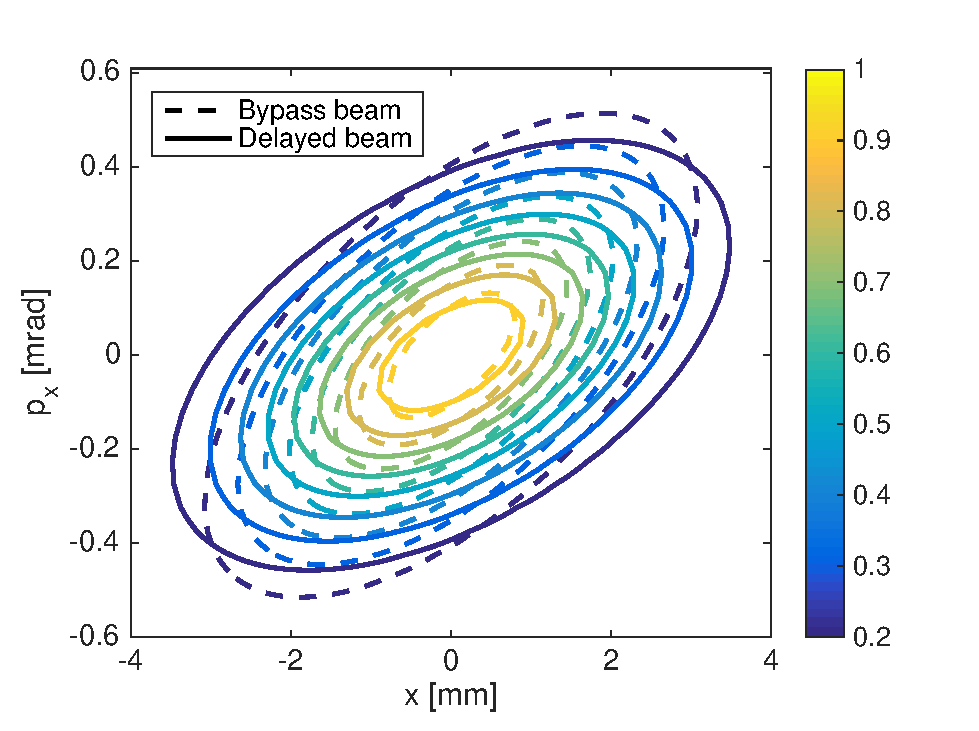
\includegraphics[width=0.45\textwidth]{DLopticsClosurefinalBeam15ghzH_quadscanTomoCentred.eps}
\label{fig:trasverseDLtomographyHQ}
}
\qquad
\subfloat[Horizontal tomography]{
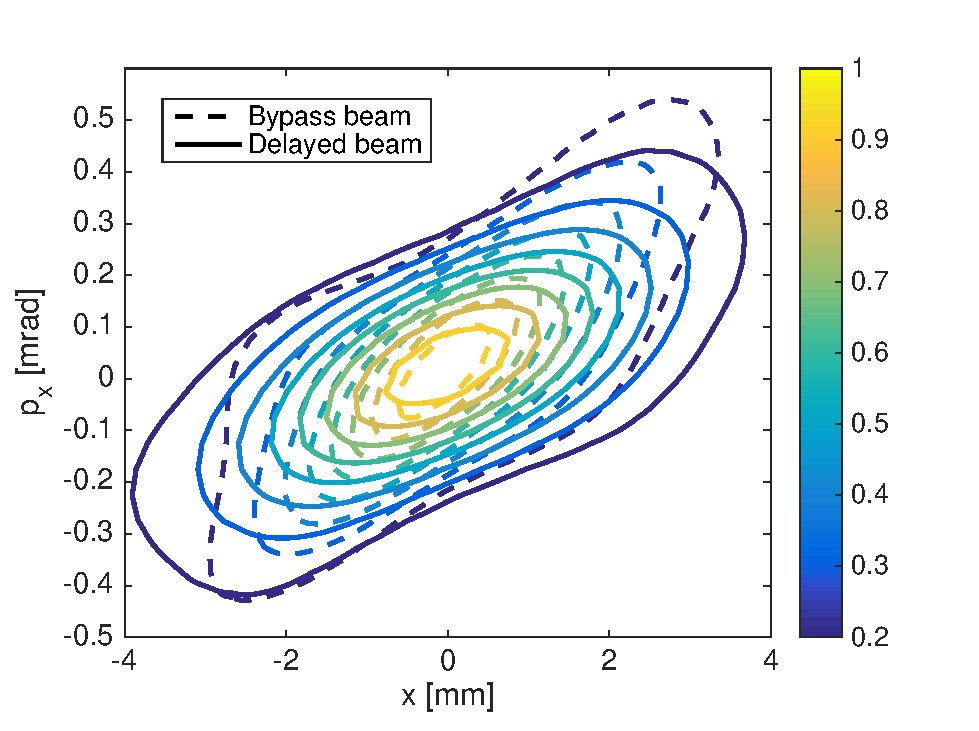
\includegraphics[width=0.45\textwidth]{DLopticsClosurefinalBeam15ghzH_tomo_biGaussianFit.eps}
\label{fig:trasverseDLtomographyHT}
}
\\
\subfloat[Vertical quadscan]{
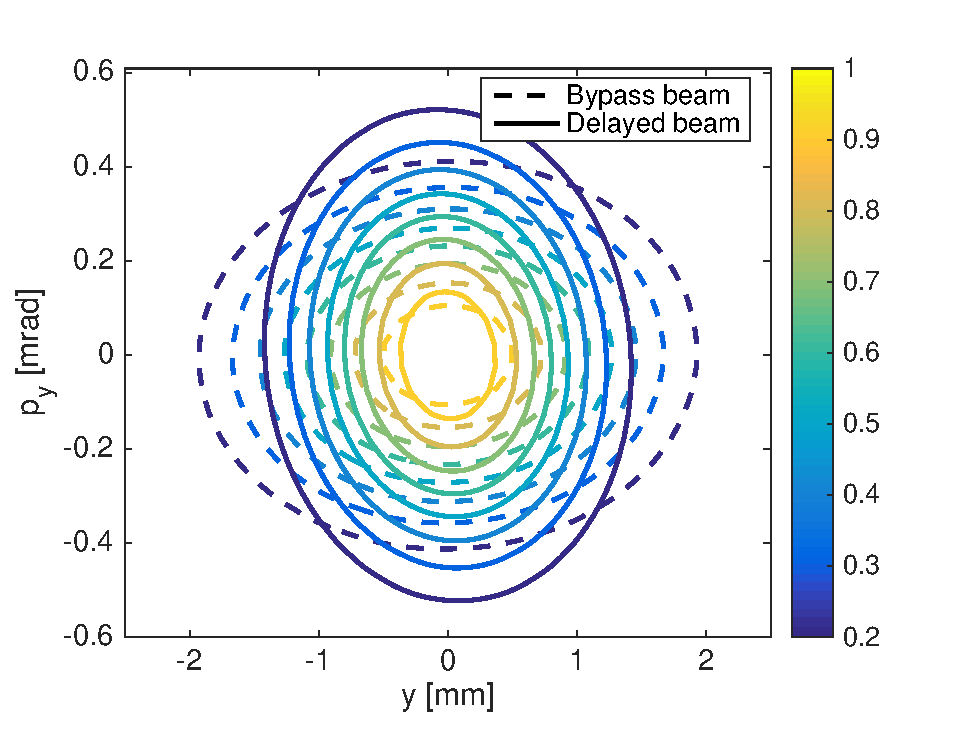
\includegraphics[width=0.45\textwidth]{DLopticsClosurefinalBeam15ghzV_quadscanTomoCentred.eps}
\label{fig:trasverseDLtomographyVQ}
}
\qquad
\subfloat[Vertical tomography]{
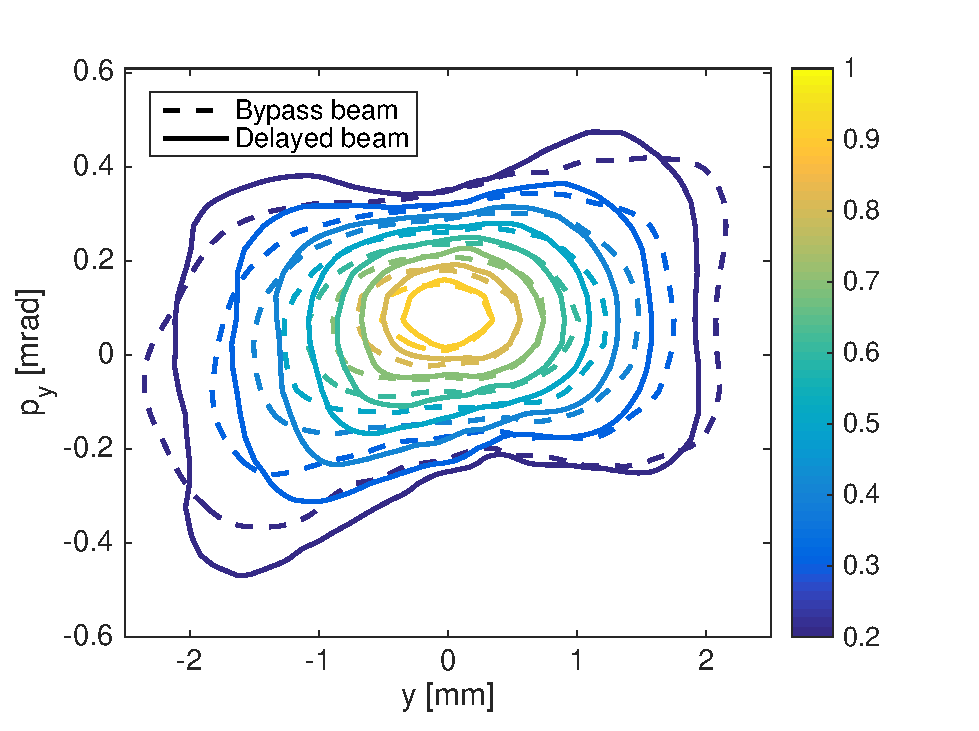
\includegraphics[width=0.45\textwidth]{DLopticsClosurefinalBeam15ghzV_tomo.eps}
\label{fig:trasverseDLtomographyVT}
}
\caption{Horizontal (\protect\subref{fig:trasverseDLtomographyHQ} and
         \protect\subref{fig:trasverseDLtomographyHT}) and vertical
         (\protect\subref{fig:trasverseDLtomographyVQ} and
         \protect\subref{fig:trasverseDLtomographyVT}) 
         phase-space distributions of the delayed and bypassing beams as measured by simple quadrupole
         scan (\protect\subref{fig:trasverseDLtomographyHQ} and
         \protect\subref{fig:trasverseDLtomographyVQ}) and tomographic
         (\protect\subref{fig:trasverseDLtomographyHT} and
         \protect\subref{fig:trasverseDLtomographyVT}) techniques.
         For both kinds of representation the same measured profile are used.
         The dashed contours represent the beam bypassing the DL, while the continuous ones are the
         distributions of the delayed beam.
         The colour code is the density distribution, which has been normalised to have a peak value
         equal to 1.
}
\label{fig:trasverseDLtomography}
\end{figure}
%
Indeed from the tomography view, especially in the vertical plane, it seems that the beam was far from
being Gaussian.
This leads to a difficult interpretation of the $\beta$ and $\alpha$ parameters measured with a
conventional quadrupole scan.
However the tomography reconstruction of the phase space suggests that the two beams are pretty well
matched with respect to each other, and the vertical $\beta$ parameter difference noted in
Table~\ref{tab:quadMatchingDL} might actually be harmless.
Still the non-Gaussian shape of the phase space might be a limiting factor for the overall performance
of the DBRC. 
A dedicated study would be needed to verify the accuracy and precision of the tomographic
measurements, which has not been performed yet.



\subsection{Dispersion corrections}

In CTF3 two methods were tried for correcting dispersion errors:
with quadrupoles, using dedicated knobs that modifed only dispersion without changing beta functions,
and Dispersion Free Steering.  
At several occations the two were compared and in CTF3 DFS was always much more efficient.
Global quadrupolar corrections that would correct simoultaneously dispersion and beta functions
were difficult to find because the beta functions were very sensitive to focusing changes
and often quadrupoles were powered in series. Also, until Phase Space Painting was 
made fully operational, precise beta function measurements were possible only 
at few locations (with quadrupolar scans using profile monitors).
Therefore, correcting first beta functions and dispersion idependently with DFS
was naturally easier. Of course, there was a risk that created orbit was
misaligned what would make sextupolar corrections tricky.

\tb{Taken from Davide's LINAC16 paper}

Figure~\ref{fig:linacDFS} shows the result of applying DFS in the CTF3 linac. 
%
\begin{figure}[!htb]
   \centering
   \includegraphics*[width=0.6\columnwidth]{MOPRC008f2.eps}
   \caption{Horizontal dispersion along the linac at CTF3.
   Black is the design dispersion.
   Red and blue are the actual dispersions measured by changing the beam energy before and after DFS respectively.}
   \label{fig:linacDFS}
\end{figure}
%
The correction was performed by first \emph{measuring} directly on the machine the response matrix of 
all dipole correctors in the linac.
Note the reduction in spurious dispersion below 5~mm.
At the same time a similar correction was performed in the vertical plane reducing 
the vertical dispersion from about 10 mm to less than 1 mm \cite{bib:DavideThesis}.
The effect of those corrections was extremely beneficial for the final beam quality.
Table~\ref{tab:TwissResultLinac} shows the Twiss parameters of the beam measured at 
the end of the linac before and after DFS in the two planes.
It is remarkable that the observed emittance was reduced by more than 15~\% in both planes, 
which is proof of the effectiveness of DFS%
\footnote{The asymmetry between the horizontal and vertical emittances was probably due to errors at the source, lately corrected by other means.}. 
%
\begin{table*}[htbp]
\centering
\caption{
Transverse Twiss parameters of the beam measured at the end of the Drive Beam linac at CTF3 before and after DFS in the linac.
Also shown are the nominal Twiss parameters for the ideal machine.}
\begin{tabular}{r c c c c c c}
\hline
				& $\beta_x$  [m]	&  $\alpha_x$ 		&  $\epsilon_{Nx}$	 [$\mu$m]	 & $\beta_y$  [m]	&  $\alpha_y$ 		&  $\epsilon_{Ny}$	 [$\mu$m]	  \\
\hline
Nominal Twiss 	& $8.4$ 			& $-0.8$ 			& -- 						& $13.5$ 			& $-0.4$ 			& -- \\
Before DFS		& $9.2 \pm 0.4$ 	& $-0.7 \pm 0.1$ 	& $\mathbf{63 \pm 1}$ 				& $11.3 \pm 1.2$	& $-0.1 \pm 0.1$	&  $\mathbf{129 \pm 8}$ \\
After DFS			& $8.7 \pm 0.4$ 	& $-0.5 \pm 0.1$ 	& $\mathbf{52 \pm 1}$ 				& $10.3 \pm 1.0$	& $-0.1 \pm 0.1$	&  $\mathbf{102 \pm 5}$ \\
\hline
\end{tabular}
\label{tab:TwissResultLinac}
\end{table*}
%


DFS was performed also in the DBRC, but clearly only in the vertical plane where 
no dispersion is expected by design.
In the horizontal plane, where dispersion is non-zero by design in most location, 
DTS has been tested.
Note that for DTS one needs first to know the target dispersion.
Naively one could try to target the design dispersion, 
however any BPM calibration issue or a wrong set up of the quadrupoles strength would 
drive the correction to an undesired state.
Here the concept of ``nominal'' dispersion previously introduced becomes extremely useful.

Figure~\ref{fig:CRDTS} shows the result of a DTS attempt in the CR at CTF3.
%
\begin{figure}[!htb]
   \centering
   \includegraphics*[width=0.6\columnwidth]{MOPRC008f3.eps}
   \caption{Horizontal dispersion along the CR at CTF3.
   Black is the design dispersion.
   Green is the ``nominal'' dispersion measured by scaling the bending magnets of the ring, and it was used as target for DTS.
   Red and blue are the actual dispersions measured by changing the beam energy before and after DTS respectively.}
   \label{fig:CRDTS}
\end{figure}
%
Note the discrepancy at $s \approx 67$ m between the design dispersion (black) and 
the measured ``nominal'' dispersion (green) due to a mis-calibration of a BPM. 
It is clear that if one would target the design dispersion at this location 
one would have driven the line toward an undesired set-up.
For this correction only dipole correctors inside the CR were used, 
therefore in the first part of the ring DTS does not have enough degrees of freedom,
but the correction starts to be effective in the second half of the ring.

DTS is a promising technique, but further experimental verification are needed to 
prove its effectiveness in improving the Drive Beam recombination quality.

%%%%%%%%%%%%%%%%%%%%%%%%%%%%%%%%%%%%%%%%%%%%%
\subsubsection{Dispersion for machine set up and optimisation}
%
One of the recent improvements of the recombination process at CTF3 was 
the optimisation of the DL optics in order to reduce the outgoing non-linear dispersion \cite{gambaIPAC16}.
The ability of measuring non-linear dispersion turned out to be useful as a verification of the improvement.
Figure~\ref{fig:DLnewOptics} shows a scatter plot of consecutive beam shots with different energies at 
the first BPM after DL for the two different optics.
%
\begin{figure}[!htb]
   \centering
   \includegraphics*[width=0.6\columnwidth]{MOPRC008f4.eps}
   \caption{Comparison of non-linear dispersion at the first BPM after the DL for two different DL optics.
   Scatter plot of the mean position recorded at the BPM versus beam energy variation.}
   \label{fig:DLnewOptics}
\end{figure}
The second order dispersion is clearly visible for both DL optics, but the effect is sensibly reduced for the new one (blue).

Another important use of the dispersion as indicator of the quality of set-up is the use of 
the ``nominal'' dispersion measurement previously introduced.
Since such a measurement is not affected by misalignments, it gives a direct measurement of 
the correctness of the quadrupole and relative dipole strengths.
Figure~\ref{fig:CRfirstarc} shows one of these measurements in the first arc of the CR.
%
\begin{figure}[!htb]
   \centering
   \includegraphics*[width=0.6\columnwidth]{MOPRC008f5.eps}
   \caption{Orbit response at the BPMs in the first arc of CR while scaling the ring dipoles.
   Black is the design dispersion.
   Coloured are actual measurements: the initial status (red) and scaling the arc quadrupoles by 
   -1\% (yellow), +2\% (purple), +3\%(green).}
   \label{fig:CRfirstarc}
\end{figure}
%
Note that in the middle of the arc one expects a dispersion close to zero, while the initial measurement (red) 
was measuring a ``nominal'' dispersion sensibly different from zero.
By scaling up the quadrupoles in the arc the pattern got closer to the design (e.g. green).
The improvement could be seen also observing the variation of the ring $R_{56}$.
As one expects to measure the nominal $D_x$ while scaling the bending magnets,
then one should be able to reveal at the same time the ``nominal'' $R_{56}$.
The optics of the CR is meant to be isochronous \cite{bib:CTF3DesignReport}.
For the purpose of beam recombination two RF deflectors are installed around the CR injection. 
After one turn in the ring the beam is expected to cross the deflectors on zero-crossing. 
Clearly if $R_{56}$ is non-zero, any variation of path length while scaling the bending magnets results in 
a visible bump in the orbit, which is seen by the dispersion monitor application as actual ``nominal'' dispersion.
Figure~\ref{fig:CRRFbump} shows this effect during the optimisation of the arc quadrupole strengths presented in 
Figure~\ref{fig:CRfirstarc}.
%
\begin{figure}[!htb]
\centering
   \begin{tikzpicture}
      \node[anchor=south west,inner sep=0] (image) at (0,0) {\includegraphics*[width=0.6\columnwidth]{MOPRC008f6.eps}};
      \begin{scope}[x={(image.south east)},y={(image.north west)}]
        \draw [dashed, thick, blue] (0.24,0.17) -- (0.24,0.9);
        \draw [dashed, thick, blue] (0.80,0.17) -- (0.80,0.9);
        %
        \node[below, align=center, blue, fill=white] at (0.24,0.9) {\footnotesize RF def. 2};
        \node[below, align=center, blue, fill=white] at (0.80,0.9) {\footnotesize RF def. 1};
      \end{scope}
   \end{tikzpicture}
   \caption{Orbit response at the BPMs around the RF deflectors of the CR while scaling the ring dipoles for 
            the same set-ups of Figure~\ref{fig:CRfirstarc}.
            The additional blue measurement was performed with the initial quadrupole strengths but 
            without RF into the deflectors.}
   \label{fig:CRRFbump}
\end{figure}
%
Note that also in terms of $R_{56}$ by scaling up the arc quadrupoles the optics got closer to nominal.
As a proof that the effect was really given by the lengthening of the beam path, 
note that when RF was removed from the deflector the effect disappeared (see blue curve in Figure~\ref{fig:CRRFbump}).

From Figure~\ref{fig:CRRFbump} one can be more quantitative: the orbit excursion expected with the RF bump can be written as:
\begin{equation}
\Delta x \approx R_{56} \frac{\Delta p}{p_0} \frac{2 \pi}{\lambda_{RF}} x_{max}.
\label{eq:orbitErrorDueToR56}
\end{equation}
%
where $\lambda_{RF}$ is the RF wavelength and $x_{max}$ is the maximum orbit excursion expected when 
the beam is crossing the cavities on crest. 
By scaling the bending magnets one actually measures the overall linear coefficient of 
Eq.~\ref{eq:orbitErrorDueToR56} with respect to 
$\Delta p/p_0$.
By knowing that $x_{max}\approx 25$ mm; $\lambda_{RF}\approx 10$ cm one can than estimate 
$R_{56} \approx 0.16$~m before the correction (red) and $R_{56} \approx 0.04$~m after the correction (green).



%%%%%%%%%%%%%%%%%%%%%%%%%%%%%%%%%%%%%%%%%%%%%
\subsubsection{Conclusions}
%
\todo[inline]{Move to final conclusions}
The ability of measuring and controlling dispersion in the different beam lines has been demonstrated.
A series of examples has proven the potential of using dispersion not only for beam steering (DFS and DTS),
but also as a mean for optics optimisation.


\subsection{Orbit Closure \label{sec:03_OrbitClosure}}



%%%%%%%%%%%%%%%%%%%%%%%%%%%%%%%%%%%%%%%%%%%%%%%%%%%%%%%%%%%%%%%%%
\subsubsection{Horizontal and vertical orbit matching}
%

Unfortunately the BPMs installed at CTF3 could not resolve the single bunch orbit, 
and it was impossible to observe directly the orbit mismatch between recombined bunches.
In case of the Delay Loop the orbit mismatch measurement was done with a pulse 
for which the first half of the train bypassed the DL, while the second half was delayed.
Than the two subpulses followed each other in TL1 and CR separated by a gap corresponding to 
the Delay Loop time of flight. It required a 280 ns-long 1.5~GHz bunch train.
The phase of the bunches had to be flipped by 180 degrees with respect to the nominal setup.
This way the second half of the train was injected to the Delay Loop instead of the first half. 
Hence, rather then combining the two sub-trains of bunches, they were separated from each other and 
their orbit difference was easily measured in the following transfer line.
Unfortunately this technique had two main disadvantages:
%
\begin{itemize}
\item
In order to perform the measurement and correction a dedicated beam had to be set-up
starting from the injector.
This meant that the measured orbit difference might not be the actual mismatch that was in
place during the factor-2 recombination.
\item
The BPMs installed in the TL1 transfer line were known to misbehave with such a beam,
providing inconsistent performances between the measurement of the delayed and bypassing
bunches. This issue is not yet fully understood.
\end{itemize}
%

In order to avoid these issues a simpler set-up was used.
The target orbit in TL1 was measured by using the nominal 1.5~GHz beam, but forcing it to
bypass the DL by switching off the RF deflector and replacing its function with two orbit corrector magnets.
This was a standard procedure to bypass the DL independently of the kind of beam that is
produced in the linac.
Afterwards the beam was magnetically injected and extracted from the DL, and its orbit in
TL1 was corrected by acting only on the correctors inside the DL. 
The magnetic injection makes use of the same correctors used to magnetically bypass the DL,
but with opposite kick.

Figure~\ref{fig:orbitCorrectionDLmatching} shows an example of horizontal~\subref{fig:orbitCorrectionDLmatchingH} and vertical~\subref{fig:orbitCorrectionDLmatchingV} orbit corrections achieved in the latest
CTF3 run of 2015.
For these corrections the variation of the DL corrector strengths is shown in
Figure~\ref{fig:correctorsCorrectionDLmatching}.
%
\begin{figure}[htbp]
  \subfloat[Horizontal]{
    \includegraphics[width=0.45\textwidth]{DLorbitclosureHobservables_delta.eps}
    \label{fig:orbitCorrectionDLmatchingH}
  }
  \qquad
  \subfloat[Vertical]{
    \includegraphics[width=0.45\textwidth]{DLorbitclosureVobservables_delta.eps}
    \label{fig:orbitCorrectionDLmatchingV}
  }
  \caption{Difference between the delayed and bypassing beam orbits in the TL1 BPMs before
           (red) and after (blue) orbit matching correction.
           \protect\subref{fig:orbitCorrectionDLmatchingH}  horizontal plane.
           \protect\subref{fig:orbitCorrectionDLmatchingV} vertical plane.
           The error bars are the statistical error on about 20 orbit measurements.
           The dashed-black lines represent the desired difference that is naturally zero.
           Note that BPM CTBPI0692 was not operational at the time of the experiment, while
           thehorizontal position in BPM CRBPI0130 was not usable due to hardware limitations.
           No values are given in these cases and dashed lines connect the points before and
           after the faulty BPMs.
  }
  \label{fig:orbitCorrectionDLmatching}
\end{figure}
%
%
\begin{figure}[htbp]
\subfloat[Horizontal]{
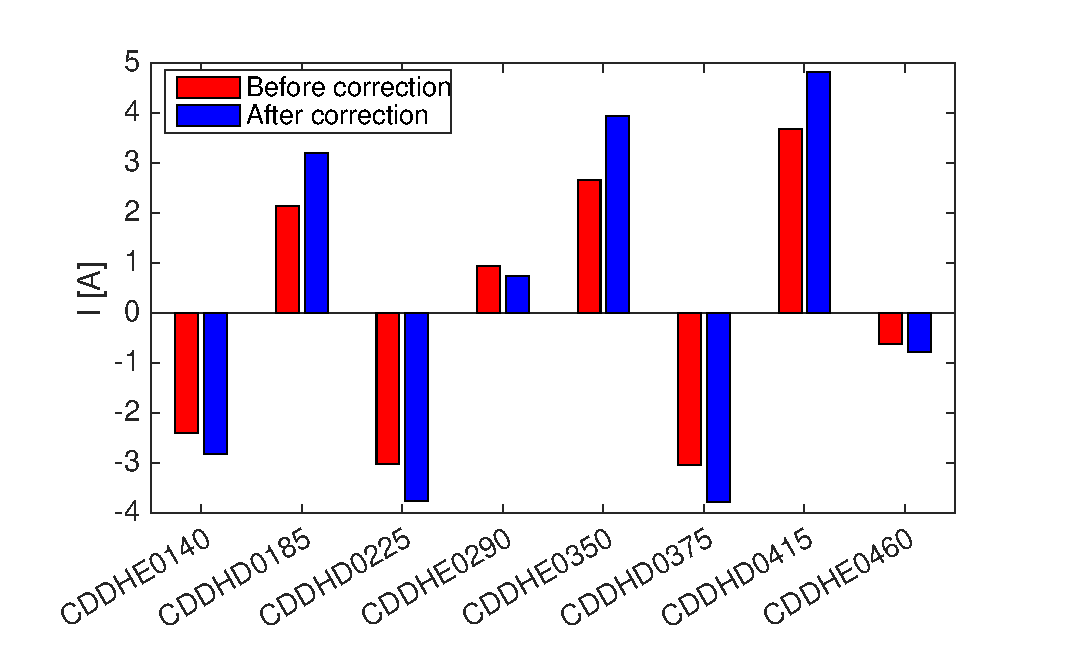
\includegraphics[width=0.45\textwidth]{DLorbitclosureHcorrectors.eps}
\label{fig:correctorsCorrectionDLmatchingH}
}
\qquad
\subfloat[Vertical]{
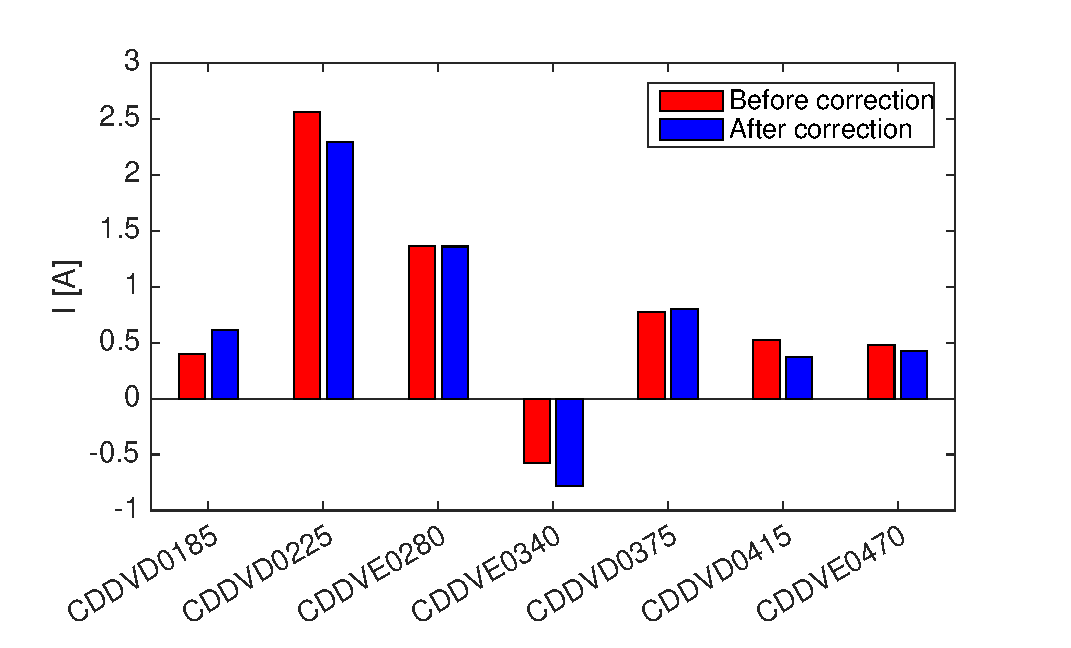
\includegraphics[width=0.45\textwidth]{DLorbitclosureVcorrectors.eps}
\label{fig:correctorsCorrectionDLmatchingV}
}
\caption{DL corrector strengths before (red) and after (blue) the orbit matching in TL1
between the delayed beam and bypassing beam. 
\protect\subref{fig:correctorsCorrectionDLmatchingH} is for to the horizontal plane, while
\protect\subref{fig:correctorsCorrectionDLmatchingV} is for the vertical one.
}
\label{fig:correctorsCorrectionDLmatching}
\end{figure}
%
The final orbit matching obtained in Figure~\ref{fig:orbitCorrectionDLmatching} has to be
compared with the tolerances derived in Section~\ref{sub:monochEffDL} and presented in
Figure~\ref{fig:orbitTolTL1}.
For both planes, if one trusts the calibrations of the BPMs, after the correction the
expected projected emittance growth is below 50\% for both definitions of emittance
presented in Section~\ref{sub:noteSimulEmit}.
A better correction appears to be challenging with the aperture constraints of the DL.
However such an emittance growth can be acceptable.

It is interesting to note in
Figure~\ref{fig:correctorsCorrectionDLmatching}\subref{fig:correctorsCorrectionDLmatchingH}
that the DL correctors are fired in an alternating pattern.
The linearFeedback application used for the correction is normally able to remove
unnecessary correction by targeting a proper correctors pattern, 
e.g. all the correctors with null strength.
Unfortunately the dynamic aperture of the DBRC at CTF3 and in particular of the DL does not
allow much freedom.
For this reason most of the corrections presented in this chapter are not targeting a null
strength on the correctors, but rather the initial corrector strengths that were
empirically found by optimising beam transmission.
However
Figure~\ref{fig:correctorsCorrectionDLmatching}\subref{fig:correctorsCorrectionDLmatchingH}
suggests that the bending magnets of the DL could have been wrongly set with respect to the
beam energy, and hence the correctors are compensating for this error.
A possible improvement of the correction could then be to use not only the correctors, but
also the strengths of the bending magnets. %, as steerers.



The next step in the beam recombination process at CTF3 is the factor-4 recombination that 
takes place in the Combiner Ring (CR).
Here a set of measurements and corrections with the aim of improving the quality of 
a pure factor-4 recombination in the CR are reported.
This means that all the results presented in this section have been obtained with 
a beam that was bypassing the DL using magnetic correctors instead of the RF deflector 
normally used for the factor-2 recombination.
The beam generated from the linac was at 3 GHz, which was then not suitable for 
the full factor-8 recombination.

Note that the reported experiments were not performed in chronological order.
Even in the chronological case, the facility could have been set up for different experiment 
from day to day, so earlier corrections and performance might not be preserved 
between different experiments. 


In the Combiner Ring there were two possibilities to inject the beam into the closed orbit:
\begin{itemize}
\item Modify the incoming orbit such that the beam is injected onto 
      the natural closed orbit of the ring.
\item Modify the closed orbit of the ring by acting on the correctors installed in 
      the ring itself, and so match the closed orbit of the ring with the incoming orbit.
\end{itemize}
%
The first method is probably the cleanest: 
one could measure the closed orbit of the ring by taking the average orbit of 
a beam circulating for many turns, hence steer the incoming beam such that 
the first turn orbit equals the closed orbit previously measured.
On the other hand this requires one to have a beam already circulating for many turns 
into the ring, and have BPMs able to measure precisely the orbit for several turns.
Normally this is not the case at CTF3. From experience at CTF3 it turns out that the most effective
approach is the second one. The orbit closure correction was performed by acting on the correctors of
the CR while minimising the difference between the orbits of the first and second turns in the ring.

Figure \ref{fig:orbitCRmatchingMeas} shows an example of such a correction.
Not all the BPMs of the CR were used, but only those in dispersion-free areas of the ring. 
This was an attempt to minimise the energy effects observed in BPMs that are normally in 
regions with high dispersion.
%
\begin{figure}[htbp]
\centering
\subfloat[Horizontal]{
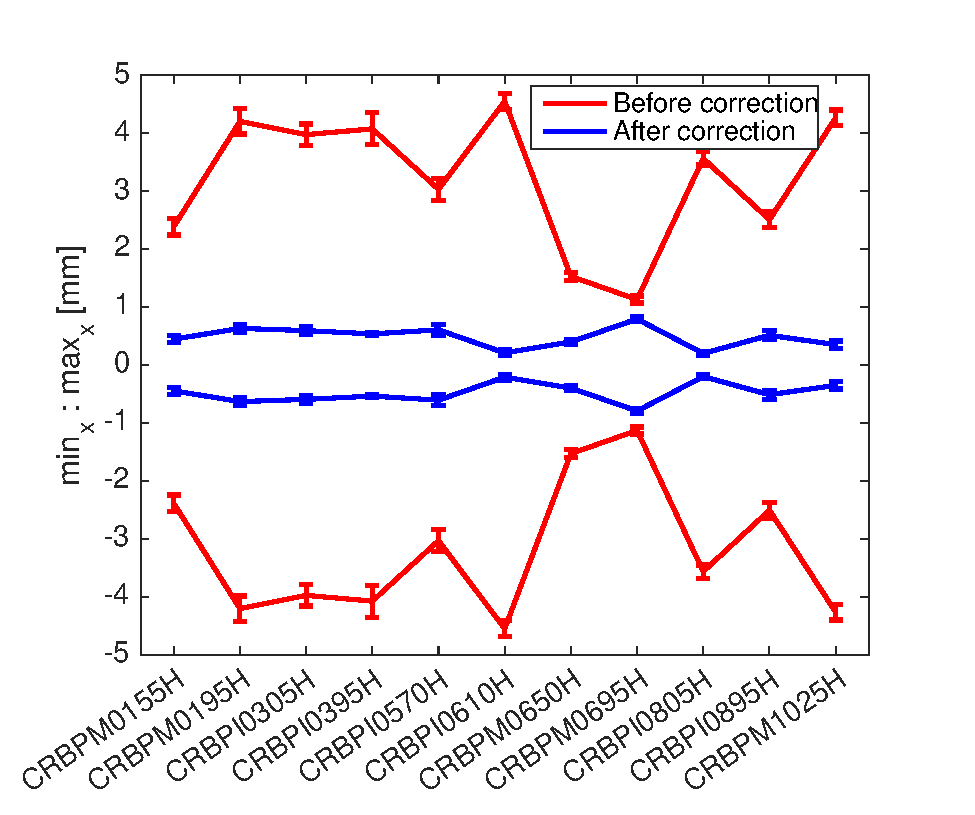
\includegraphics[width=0.45\textwidth]{CRoCloseH_corridorBeforeAfter.eps}
\label{fig:orbitCRmatchingMeasH}
}
\qquad
\subfloat[Vertical]{
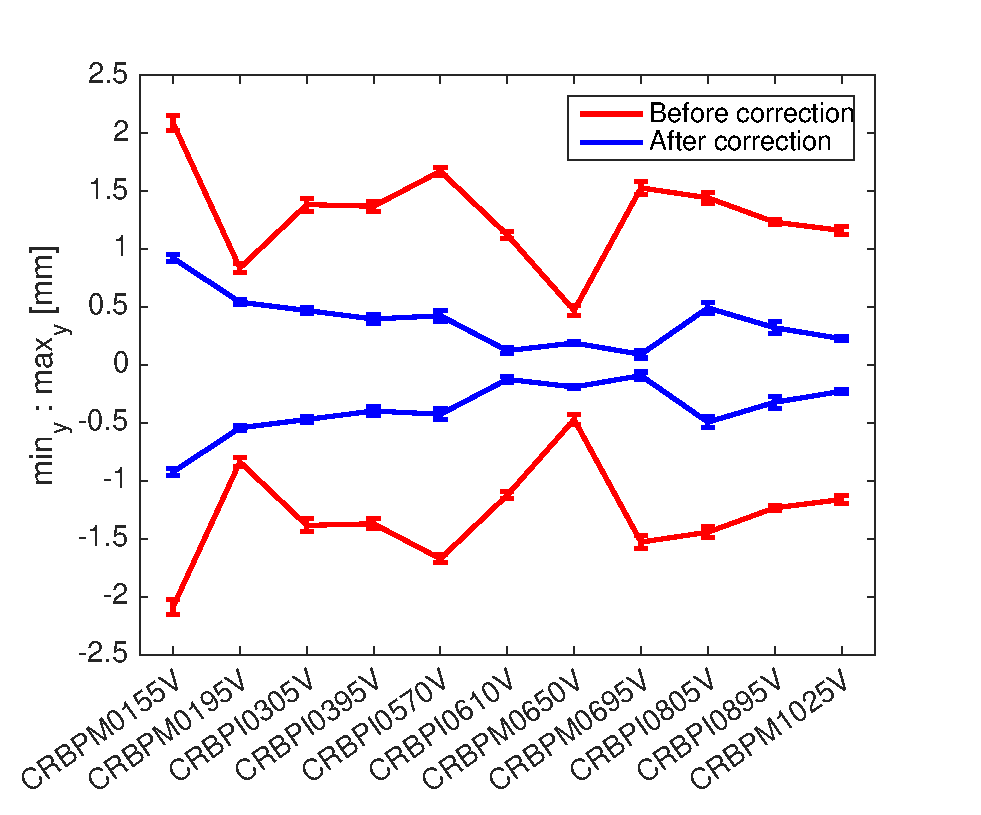
\includegraphics[width=0.45\textwidth]{CRoCloseV_corridorBeforeAfter.eps}
\label{fig:orbitCRmatchingMeasV}
}
\caption{Horizontal~\protect\subref{fig:orbitCRmatchingMeasH} and 
         vertical~\protect\subref{fig:orbitCRmatchingMeasV} orbit corridors within which
         the orbit of a beam circulating for 4 turns in the CR are confined before (red) and 
         after (blue) an orbit closure correction.}
\label{fig:orbitCRmatchingMeas}
\end{figure}
%
The strengths of the correctors that were used for the correction 
are shown in Figure~\ref{fig:orbitCRmatchingCorr}.
For the vertical plane it is important to point out that the feedback tool 
was able not only to heavily reduce the orbit mismatch, 
but also to remove the unnecessary power of the last three correctors in the ring. 
%
\begin{figure}[bp]
\centering
\subfloat[Horizontal]{
\includegraphics[width=0.45\textwidth]{CRoCloseH_correctors.eps}
\label{fig:orbitCRmatchingCorrH}
}
\qquad
\subfloat[Vertical]{
\includegraphics[width=0.45\textwidth]{CRoCloseV_correctors.eps}
\label{fig:orbitCRmatchingCorrV}
}
\caption{Strength of the horizontal~\protect\subref{fig:orbitCRmatchingCorrH} and 
         vertical~\protect\subref{fig:orbitCRmatchingCorrV} correctors in 
         the CR before (red) and after (blue) an orbit closure correction.}
\label{fig:orbitCRmatchingCorr}
\end{figure}
%
At the BPMs shown in Figure~\ref{fig:orbitCRmatchingMeas} the orbit difference between
different turns was reduced to below 1 mm in the horizontal plane and 0.5 mm in the
vertical.
The result obtained should be compared with the tolerances for an ideal machine that
were presented in Section~\ref{subs:crtollerances} (Figure~\ref{fig:orbitTolCR}).
Note that for the vertical plane the statistical emittance growth one should expect
should be below 30\%, while in the horizontal plane things are more critical, being
close to the 70\% envelope of Figure~\ref{fig:orbitTolCR}\subref{fig:orbitTolCRH}.

Unfortunately there was not enough time to systematically measure the initial and final
Twiss parameters of the different turns before and after the orbit correction presented
in Figure~\ref{fig:orbitCRmatchingMeas}.
Only for the vertical plane a measurement of the Twiss parameters of a factor-4
combined beam was taken right before and after the orbit correction presented here,
while for the horizontal plane this measurement was performed only after the orbit
correction.
For the horizontal plane one can consider as a reference the latest measurement
presented in the previous section.
Figure~\ref{fig:orbitCRmatchingQuad} shows the comparison between the beam variance for
the different scans, while the fitted Twiss parameters are reported in
Table~\ref{tab:orbitCRmatchingQuad}.
%
\begin{figure}[b!p]
\centering
\subfloat[Horizontal]{
\includegraphics[width=0.45\textwidth]{CRoCloseH_oldBefore_AfterComparisonQuadscan271.eps}
\label{fig:orbitCRmatchingQuadH}
}
\qquad
\subfloat[Vertical]{
\includegraphics[width=0.45\textwidth]{CRoCloseV_beforeAfterQuadscan271.eps}
\label{fig:orbitCRmatchingQuadV}
}
\caption{Beam variance measured at the screen CC.MTV0253 in TL2 as a function of
         the quadrupole current used to perform quadrupole scan measurements
         in the horizontal \protect\subref{fig:orbitCRmatchingQuadH} and vertical
         \protect\subref{fig:orbitCRmatchingQuadV} plane.
         The red points are relative to a combined factor-4 beam before orbit
         closure correction, while in blue is the same scan after the correction
         presented in Figure~\ref{fig:orbitCRmatchingMeas}.
         The error bars are computed from the Gaussian fits to the profiles
         measured at the screen.
         The dashed lines are the fits to the data corresponding to the Twiss
         parameters that are reported in Table~\ref{tab:orbitCRmatchingQuad}.
         Note that the red scan in the horizontal plane was performed a few days
         before the orbit correction.}
\label{fig:orbitCRmatchingQuad}
\end{figure}
%
%
\begin{table}
\centering
\begin{tabular}{l c c c c c c}
\hline
                     & $\beta_x$  [m]  &  $\alpha_x$     &  $\epsilon_{Nx}$   [$\mu$m]   & $\beta_y$  [m]  &  $\alpha_y$     &  $\epsilon_{Ny}$   [$\mu$m]    \\
\hline
Nominal values       & $8.9$       & $-7.2$       & --             & $4.8$       & $0$       & -- \\
Before correction    & $4.1 \pm 0.4$   & $-2.9 \pm 0.3$   & $234 \pm 9$         & $7.2 \pm 0.7$   & $-1.4 \pm 0.2$   & $66 \pm 3$ \\ 
After correction     & $7.1 \pm 0.3$   & $-5.3 \pm 0.3$   & $173 \pm 4$         & $6.7 \pm 1.3$   & $-1.5 \pm 0.4$   & $37 \pm 3$ \\
\hline
\end{tabular}
\caption{Comparison between Twiss parameters of a factor-4 beam measured at 
         screen CC.MTV0253 before and after orbit closure in the CR.
         Note that for the horizontal plane the measurement was performed 
         a few days before the correction.
}
\label{tab:orbitCRmatchingQuad}
\end{table}
%
In the vertical plane the effect of the orbit correction is clear, and
it results in almost a factor-2 reduction of the overall emittance.
For the horizontal plane, as already stated, no measurement right
before the correction is available, so it is possible that many
parameters could have changed between the quadrupole scan measurements.
Still a 25\% emittance reduction is visible and also the Twiss
parameters $\alpha_x$ and $\beta_x$ seem to get closer to the nominal
values. 

In general one can state that the orbit closure correction brings an
evident benefit in the combined beam quality, which is still believed
to be one of the main source of emittance growth in the CR.











\subsection{Emittance control in the Injector: Strength of the solenoids in the beginning of the linac \textbf{(Tobias, Davide and Roberto)}}

A major challenge in CTF3 is to limit the emittance increase. There are different ways the emittance can be increased. 






%%%%%%%%%%%%%%%%%%%%%%%%%%%%%%%%%%%%%%%%%%%%%
% RESULTS: Emittance
\section{Best ever achieved emittance}

The quest to minimize the drive beam emittance continued all along the CTF3 lifetime 
and indeed for the nominal factor 8 recombined beam the lowest value was recorded on the very last day of operation.
The measurements presented here are the best values achieved at given location. 
The values correspond to 1~\textsigma~ normalized emittance.

The machine drifts made this tusk very difficult. 
During the initial years it was virtually impossible to systematically optimize the beam optics 
and the orbit because measurements and optimizations were becoming obsolete within less than one hour.
Only in 2014 the machine achieved sufficient stability levels so the beam performance 
optimizations gave the expected results and the improved beam quality could be maintained 
over time. 

Required optimizations at the injector level, 
but also relatively frequent failures of the RF sources,
meant that beam parameters in the injector and the linac were periodically changed.
These made the previous optimizations invalid and 
meant that the setup had to be redone all along the machine.
Here important factor was also the time needed for measurements and preparation of the corrections.
The most crucial measurements, quadrupolar scans and dispersion, took tens of minutes.
Naturally, the software tools helped to automatize most of the tasks, 
however, they were developed already during the machine operation
and some of them become available relatively late.


\subsection{Emittance evolution \label{sec:emittancemeasured}}

Table~\ref{tab:emittancesummary} lists the achieved emittances along the machine.
One can find more dowstream values are sometimes smaller than the upstream ones.
This observetion was not uncommon at CTF3 and there are several effects that explain this.
First, the measured beam size is affected by nonlinearites and 
they can be differently pronounced at different locations. It was specially true 
for the drive beam with 0.6\% energy spread combined with a strong isochronous optics.
Socond, it can not excluded that some small part of the beam was scraped in the transport.
Even though the calibration of the BPMs was carefully done, 
their overal accuracy was at the order of 10\%. 
Finally, the systematic errors of the quadrupolar scans is within tens of percent. 
\todo[inline]{Add this to QS section (paragraph about QuadScan systematic uncertainty) }
Repeating the same measurement normally was giving results with \textpm5\% spread and 
using different ranges for quadrupole strengths sometimes gave 50\% different results.
Of course, this was an indication of an error in the hardware or in the computer program.
It was verified multiple times and the software was tested with simulated data.

% 1.5GHz 
  % Linac 
    %  H  59 with switches http://elogbook.cern.ch/eLogbook/eLogbook.jsp?lgbk=100&date=20160509
    %  V  40     several measurements on that day (following day 70/45 H/V)
    %  H  57  http://elogbook.cern.ch/eLogbook/event_viewer.jsp?eventId=1794890 (2014)
    %  V  51  http://elogbook.cern.ch/eLogbook/event_viewer.jsp?eventId=2118848  30-May-2016
  % DLin 
    %  H  57  http://elogbook.cern.ch/eLogbook/event_viewer.jsp?eventId=2225942
    %  H  68  http://elogbook.cern.ch/eLogbook/event_viewer.jsp?eventId=2113239 and 67 the same day (18-May-2016)
    %  H  67  http://elogbook.cern.ch/eLogbook/event_viewer.jsp?eventId=1797783 (03-Apr-2014)
    %  H  72  http://elogbook.cern.ch/eLogbook/event_viewer.jsp?eventId=1798385 (14-Apr-2014)
    %  V  76  http://elogbook.cern.ch/eLogbook/event_viewer.jsp?eventId=2113196 and 2 other measurements at 90 (18-May-2016)
    %  V  63  http://elogbook.cern.ch/eLogbook/event_viewer.jsp?eventId=1798386 (14-Apr-2014)
    %  H  55  http://elogbook.cern.ch/eLogbook/event_viewer.jsp?eventId=1854639  (18-Nov-2014)
    %  V  gingin 40-50 series of crappy scans  17-05-2016
  % DLex 
    %  H  91  http://elogbook.cern.ch/eLogbook/event_viewer.jsp?eventId=2225940  (06-Dec-2016)
    %  V 125  http://elogbook.cern.ch/eLogbook/event_viewer.jsp?eventId=2225941  (06-Dec-2016)
    %  V  76  http://elogbook.cern.ch/eLogbook/event_viewer.jsp?eventId=1797777  (2014)
    % 
  %
  % CRej 
    % H 65   http://elogbook.cern.ch/eLogbook/event_viewer.jsp?eventId=2218270 22-Nov-2016
    % V 90   http://elogbook.cern.ch/eLogbook/event_viewer.jsp?eventId=2228055
  % CLEX
    %  H 270  http://elogbook.cern.ch/eLogbook/event_viewer.jsp?eventId=1796347
    %  V 110  http://elogbook.cern.ch/eLogbook/event_viewer.jsp?eventId=1796338 (2014)
    %  H 150  http://elogbook.cern.ch/eLogbook/event_viewer.jsp?eventId=1796888 
    %  V 100   --//--
    

% 3GHz
  % Linac
    %         no good measurements in 2016 
    %  H  58  http://elogbook.cern.ch/eLogbook/event_viewer.jsp?eventId=1833447   (2014)
    %  H  53  http://elogbook.cern.ch/eLogbook/event_viewer.jsp?eventId=1958366  (2015.07.01)
    %         two other ones at 60
    %  V  56  http://elogbook.cern.ch/eLogbook/event_viewer.jsp?eventId=1833452 
    %  V  41-50  http://elogbook.cern.ch/eLogbook/event_viewer.jsp?eventId=1958361 and around (2015.07.01)
    %            1 measurment at 41 and several others at 50-51
  % DLin 
    % H  66,75 http://elogbook.cern.ch/eLogbook/eLogbook.jsp?lgbk=100&date=20160726 (2016)  Other sets confirming these results on 0726 
    % V  75,80   on 0727 http://elogbook.cern.ch/eLogbook/eLogbook.jsp?lgbk=100&date=20160727 (2016)
  %               on 0807 http://elogbook.cern.ch/eLogbook/event_viewer.jsp?eventId=2156401 (2016)
  % CRej 3GHz 
    % H 105 http://elogbook.cern.ch/eLogbook/event_viewer.jsp?eventId=2227257 09-Dec-2016
    % H 79  http://elogbook.cern.ch/eLogbook/event_viewer.jsp?eventId=2227299 09-Dec-2016
    % H 80  http://elogbook.cern.ch/eLogbook/event_viewer.jsp?eventId=2227415 09-Dec-2016
    % V 47  http://elogbook.cern.ch/eLogbook/event_viewer.jsp?eventId=2227258 09-Dec-2016
    % V 64  http://elogbook.cern.ch/eLogbook/event_viewer.jsp?eventId=2181929 20-Sep-2016
  %  
  % CLEX 
    % H 112 (2016) http://elogbook.cern.ch/eLogbook/event_viewer.jsp?eventId=2177822
    % H 83  (2015) http://elogbook.cern.ch/eLogbook/event_viewer.jsp?eventId=1959321
    % V 68  (2015) http://elogbook.cern.ch/eLogbook/event_viewer.jsp?eventId=1959324
    % V     (2016) http://elogbook.cern.ch/eLogbook/eLogbook.jsp?lgbk=100&date=20160920  
    %               series of 3 qs but need to be merged and reprocessed 
    % V 73   http://elogbook.cern.ch/eLogbook/event_viewer.jsp?eventId=2161778  (2016) 
    %       not the best one, can be combined with previous ones 
\todo[inline]{There is problem with 1.5GHz measurements in CC, in 2016 there is not much, and before camera was badly calibrated.}
\begin{table}[h]
 \centering
  \begin{tabular}{lcccc}
    \hline
    {\multirow{3}{*}{Location}}& \multicolumn{4}{c}{Emittance [mm mrad]}  \\
                               & \multicolumn{2}{c}{1.5~GHz}  & \multicolumn{2}{c}{3~GHz}           \\
                               & Horizontal   &   Vertical  & Horizontal & Vertical       \\
    \hline \hline
               Linac           &  59   &  40  &  53  &  41     \\
               DL injection    &  57   &  76  &  66  &  75     \\
               DL extraction   &  90   & 126  &   -  &   -     \\
               CR extraction   &  65   &  90  &  79  &  47     \\
               CLEX            & 150   & 100  &  83  &  68     \\
    \hline
  \end{tabular}
\caption{Record emittance measurements of a not combined drive beam along CTF3.}
\label{tab:emittancesummary}
\end{table}
% f4 intensity comparison between Straight and DL http://elogbook.cern.ch/eLogbook/attach_viewer.jsp?attach_id=1602813

Table \ref{tab:emittancevsturns} shows the emittance growth in function of turns
that the beam made in the Combiner Ring. We quote growth in percents because 
the screen was not accurately calibrated during this particular measurement. 

Behind the Combiner Ring, for the beam making only half a turn, emittance was 80~mm~mrad.
For the beam making 3 or 4 turns it was 120~mm~mrad in the best case, 
and routinly it was in range of 140-170~mm~mrad. 
The principal reason was dispersion wave created by the RF bump on the fourth turn.
In the vertical plane the growth was much smaller and values below 80~mm~mrad were measured.
In CLEX the lowest values ranged between 80 and 140 in function of turns in the ring. 
In the horizontal plane the emittance was growing in function of turns to 150 - 200~mm~mrad
and it was not possible to reduce it simultaneously for all the sub-trains. 
Finally it was understood that the beam was loosing energy in the combiner ring
due to the orbit that was not properly centered in the RF~deflectors. 
It was found only during the last months of the operation and 
when it was corrected the combined beam emittance was reduced (factor 4 from 350 to 250~mm~mrad), 
however, there was not enough time to repeat the detailed turn-by-turn emittance measurements at CLEX.


%%%%%%%%%%%%%%%%%%%%%%%%%%%%%%%%%%%%%%%%%%%%%%%%%%%%%%%%%%%%%
%%%%%%%%%%%%%%%%%%%%%%%%%%%%%%%%%%%%%%%%%%%%%%%%%%%%%%%%%%%%%
%%%%%%%%%%%%%%%%%%%%%%%%%%%%%%%%%%%%%%%%%%%%%%%%%%%%%%%%%%%%%
%%%%%%%%%%%%%%%%%%%%%%%%%%%%%%%%%%%%%%%%%%%%%%%%%%%%%%%%%%%%%
 %% Transverse closure between different turns in CR
% summary of quadscans on 3/12/2015 for a factor 2 beam circulating in CR (and final factor 8)
% study in girder 271 with no intervention on CR closure.
%%  %turns   betax           alfax          emitx                   chix    file
%%  0.5     2.84 +/- 0.45   -2.78 +/- 0.49  120.43 +/- 7.56         91.61   eh7363020342.dat
%%  1.5     4.59 +/- 0.38   -3.20 +/- 0.28  228.26 +/- 8.04         28.73   eh7363020523.dat   USELESS
%%  2.5     3.83 +/- 0.51   -2.99 +/- 0.43  175.98 +/- 9.69         198.55  eh7363020539.dat
%%  3.5     6.93 +/- 2.06   -5.13 +/- 1.59  256.27 +/- 35.13        366.33  eh7363020297.dat
%%  fact8   5.71 +/- 0.39   -4.48 +/- 0.32  399.44 +/- 13.28        47.44   eh7363020367.dat
%%  %Vertical scan
%%  %turns   betay   alfay   emity   chiy    file
%%  0.5     3.30 +/- 0.29   -0.86 +/- 0.10  23.15 +/- 0.85  26.15   ev7363020472.dat
%%  1.5     4.85 +/- 0.62   -1.09 +/- 0.16  23.40 +/- 1.18  193.92  ev7363020510.dat
%%  2.5     2.82 +/- 0.30   -0.41 +/- 0.09  35.36 +/- 1.76  30.99   ev7363020572.dat
%%  3.5     not done :(
%%  fact8   3.19 +/- 0.38   -0.87 +/- 0.14  65.33 +/- 3.10  32.43   ev7363020382.dat
%%  
%%  %%  
%%  %% Tobias did some study on 271 on 23/10/2015 (3GHz beam)
%%  % vertical
%%  filename  =  'ev7362604057.dat'; % 1 turn in ring ey = 24
%%  filename  =  'ev7362604252.dat'; % 2 turn in ring ey = 38
%%  filename  =  'ev7362604215.dat'; % 3 turn in ring ey = 57
%%  filename  =  'ev7362604169.dat'; % 4 turn in ring ey = 38
%%  filename  =  'ev7362604310.dat'; % 4 turn in ring ey = 42
%%  % horizontal
%%  filename  =  'eh7362604389.dat'; % 1 turn in ring ex = 72
%%  filename  =  'eh7362604407.dat'; % 2 turn in ring ex = 99
%%  filename  =  'eh7362604441.dat'; % 3 turn in ring ex = 98
%%  filename  =  'eh7362604352.dat   % 4 turn in ring ex = 157
%%  filename = 'eh7362604507.dat'; % 4 turn in ring ex=281
%%  % combined beam
%%  filename = 'eh7362606256.dat'; % H 234
%%  filename = 'ev7362606282.dat'; % V 67
%%  
%%  
%%  %% effect of DL beam on factor 8 in girder 300.
%%  % girder 300 factor 8 (15/12/2015 morning) HV with/without DL beam.
%%  filename = 'eh7363134691.dat'; -%%  466 emit
%%  filename = 'ev7363134720.dat'; -%%  199 emit
%%  % same, but killing DL
%%  filename = 'eh7363134732.dat'; -%%  371 emit
%%  filename = 'ev7363134743.dat'; -%%  194 emit
%%         
%%  09.12.2016
%%  H  1T 106  http://elogbook.cern.ch/eLogbook/event_viewer.jsp?eventId=2227257  beta x   11.78 +/- 1.04 alpha x  -8.25 +/- 0.73 emittance x 105.97 +/- 3.81 
%%  H  2T 108  http://elogbook.cern.ch/eLogbook/event_viewer.jsp?eventId=2227254  beta x    8.35 +/- 1.60 alpha x  -5.98 +/- 1.18 emittance x 108.18 +/- 8.31 
%%  H  3T 176  http://elogbook.cern.ch/eLogbook/event_viewer.jsp?eventId=2227250  beta x    6.42 +/- 1.50 alpha x  -4.38 +/- 1.08 emittance x 176.06 +/- 15.55 
%%  H  4T 158  http://elogbook.cern.ch/eLogbook/event_viewer.jsp?eventId=2227248  beta x    9.04 +/- 1.20 alpha x  -6.16 +/- 0.84 emittance x 157.88 +/- 8.02
%%           
%%  V  1T  46  http://elogbook.cern.ch/eLogbook/event_viewer.jsp?eventId=2227258  beta y    9.55 +/- 0.55 alpha y  -2.44 +/- 0.16 emittance y 45.56 +/- 1.60 
%%  V  2T  97  http://elogbook.cern.ch/eLogbook/event_viewer.jsp?eventId=2227255  beta y    5.07 +/- 0.21 alpha y  -1.53 +/- 0.07 emittance y 96.82 +/- 1.64 
%%  V  3T  99  http://elogbook.cern.ch/eLogbook/event_viewer.jsp?eventId=2227252  beta y   11.02 +/- 1.43 alpha y  -3.89 +/- 0.52 emittance y 98.72 +/- 5.91
%%  V  4T  54  http://elogbook.cern.ch/eLogbook/event_viewer.jsp?eventId=2227249  beta y    5.25 +/- 0.28 alpha y  -1.66 +/- 0.09 emittance y 54.37 +/- 1.15 





% 2016 Dec 12 turns
\begin{table}[]
 \centering
  \begin{tabular}{ccc}
    \hline
     Turn  & Horizontal & Vertical \\
           & [\%]       & [\%] \\
    \hline
    \hline                      
     1\nicefrac{1}{2}  &  2   & 53	 \\
     2\nicefrac{1}{2}  &  40  & 54	 \\
     3\nicefrac{1}{2}  &  33  & 16	 \\

    \hline
  \end{tabular}
\caption{Emittance growth of not combined drive beam in function of number of turns in CR with respect 
         of the beam extracted after \nicefrac{1}{2} turn.}
\label{tab:emittancevsturns}
\end{table}
%% Using data of 23/10/2015
%\begin{table}[]
% \centering
%  \begin{tabular}{ccc}
%    \hline
%    Turn  & Horizontal & Vertical \\
%           & [\%]       & [\%] \\
%    \hline
%    \hline
%     1\nicefrac{1}{2}  &  38   &   58    \\
%     2\nicefrac{1}{2}  &  36   &   138   \\
%     3\nicefrac{1}{2}  &  118  &   58    \\
%    \hline
%  \end{tabular}
%\caption{Emittance growth of not combined drive beam in function of number of turns in CR with respect 
%         of the beam extracted after \nicefrac{1}{2} turn.}
%label{tab:emittancevsturns}
%\end{table}



\subsubsection{Transverse matching}

Example results of the transverse matching for the beam combined in the Delay Loop is 
shown in Table~\ref{tab:DLTransvClosure}. 
In the Combiner Ring it was much more difficult to correct the beating,
see section refToSection for the procedure details.
The procedure was very long because all 4 turns had to be measured at each iteration,
such that only one iteration was done in most of the cases. 
Table~\ref{tab:CRTransvClosure} shows example results.

In the Delay Loop it was possible to match the orbits for the combined beams within XX~mm in the horizontal plane 
and XX~mm in the vertical one what corresponds to more or less 0.5~\textsigma~. 
In case of CR it was respectively cXX and cYY? 


%\textbeta-functions Taking into account the stabiliuty of the measured parameters the 

%
% Factor 2  2016-Dec-2016
  % H 152(+154)   http://elogbook.cern.ch/eLogbook/event_viewer.jsp?eventId=2229045
  % V 198         http://elogbook.cern.ch/eLogbook/event_viewer.jsp?eventId=2229046
% DL 08-Dec-2015
  % H st 102  7.61  -0.78   http://elogbook.cern.ch/eLogbook/event_viewer.jsp?eventId=2053610
  % H dl 112  8.92  -0.60   http://elogbook.cern.ch/eLogbook/event_viewer.jsp?eventId=2053605
  % V st  55  2.36   0.01   http://elogbook.cern.ch/eLogbook/event_viewer.jsp?eventId=2053609
  % V dl  66  4.59  -0.03   http://elogbook.cern.ch/eLogbook/event_viewer.jsp?eventId=2053611
  
%  DL 2016-Nov-21
  % H x2 beta x   7.92 +/- 0.31  alpha x  -0.58 +/- 0.03  emittance x 128.05 +/- 2.15
  % H st beta x   7.67 +/- 0.27  alpha x  -0.32 +/- 0.02  emittance x 63.36 +/- 0.88
  % H dl beta x   10.40 +/- 1.75 alpha x  -0.70 +/- 0.14  emittance x 225.43 +/- 17.95 

%  DL 06-Dec-2016
  % H st beta x   6.32 +/- 0.25 alpha x  -0.24 +/- 0.02  emittance x 55.63 +/- 0.83      http://elogbook.cern.ch/eLogbook/event_viewer.jsp?eventId=2225942
  % H dl beta x   6.31 +/- 0.90 alpha x  -0.80 +/- 0.11  emittance x 90.64 +/- 4.87      http://elogbook.cern.ch/eLogbook/event_viewer.jsp?eventId=2225941
  % H x2 beta x   7.00 +/- 0.83 alpha x  -0.25 +/- 0.07  emittance x 120.07 +/- 5.64     http://elogbook.cern.ch/eLogbook/event_viewer.jsp?eventId=2225951
  % 
  % V st beta y   9.01 +/- 0.11 alpha y  -0.15 +/- 0.01  emittance y 188.75 +/- 1.27     http://elogbook.cern.ch/eLogbook/event_viewer.jsp?eventId=2225943
  % V dl beta y   9.18 +/- 0.70 alpha y  -0.65 +/- 0.06  emittance y 125.68 +/- 5.70     http://elogbook.cern.ch/eLogbook/event_viewer.jsp?eventId=2225942
  % V x2 beta y   9.33 +/- 0.52 alpha y  -0.33 +/- 0.04  emittance y 182.51 +/- 5.81     http://elogbook.cern.ch/eLogbook/event_viewer.jsp?eventId=2225952
\begin{table}[h!]
 \centering
 \caption{Achieved Twiss Parameters closure for the Delay Loop}
 \begin{tabular}{ l c c c c c}
  \hline
    	& $\beta_x$ [m]   & $\alpha_y$   & $\beta_y$ [m]  & $\alpha_y$         \\
  Bypass beam	& 6.32 \textpm ~0.25  & -0.24 \textpm 0.02 & 9.01 \textpm 0.11 & -0.15 \textpm 0.01  \\
  Delayed beam	& 6.31 \textpm ~0.90  & -0.80 \textpm 0.11 & 9.18 \textpm 0.70 & -0.65 \textpm 0.06  \\
  Combined beam	& 7.00 \textpm ~0.83  & -0.25 \textpm 0.07 & 9.33 \textpm 0.52 & -0.33 \textpm 0.04  \\
  \hline
 \end{tabular}
 \label{tab:DLTransvClosure}
\end{table}


\begin{table}[h!]
 \centering
 \caption{Example results for Twiss Parameters closure for the Combiner Ring}
 \begin{tabular}{ l c c c c c}
  \hline
    Turn	& $\beta_x$ [m]   & $\alpha_y$   & $\beta_y$ [m]  & $\alpha_y$         \\
  \nicefrac{1}{2}	& 11.78 \textpm ~1.04  & -8.25 \textpm ~0.73 &  9.55 \textpm ~0.55 & -2.44 \textpm ~0.16  \\
  1\nicefrac{1}{2}  &  8.35 \textpm ~1.60  & -5.98 \textpm ~1.18 &  5.07 \textpm ~0.21 & -1.53 \textpm ~0.07  \\
  2\nicefrac{1}{2}  &  6.42 \textpm ~1.50  & -4.38 \textpm ~1.08 & 11.02 \textpm ~1.43 & -3.89 \textpm ~0.52  \\
  3\nicefrac{1}{2}  &  9.04 \textpm ~1.20  & -6.16 \textpm ~0.84 &  5.25 \textpm ~0.28 & -1.66 \textpm ~0.09  \\
  \hline
 \end{tabular}
 \label{tab:CRTransvClosure}
\end{table}





\subsection{Combined beam emittance}

%%%%%%%%%%%%%%%%%%%%%%%%%%%%%%%%%%%%%%%%%%%%%%%%%%%%%%%%%%%%%%%%%%%%%%%%%%%%%%%%%%%%%%%%%%%%%%%%%%%%%
% F8 girder 27
%%%%%%%%%%%%%%%%%%%%%%%%%%%%%%%%%%%%%%%%%%%%%%%%%%%%%%%%%%%%%%%%%%%%%%%%%%%%%%%%%%%%%%%%%%%%%%%%%%%%%
% Vertical 120 mm mrad with ~27A beam 
%    http://elogbook.cern.ch/eLogbook/event_viewer.jsp?eventId=2228935
%     corresponding transmission meas http://elogbook.cern.ch/eLogbook/event_viewer.jsp?eventId=2228936
% V 138 mm mrad                    on 2014 May 13 12h09  http://elogbook.cern.ch/eLogbook/event_viewer.jsp?eventId=1800616


The lowest achieved emittance for factor 8 recombined beam  was 243~mm~mrad for horizontal plane
and 120~mm~mrad for vertical plane.
Figure~\ref{fig:record_low_factor8_girder27} shows the results of the respective quadrupole scan measurements 
at the beginning of the TL2 line with screen CC.MTV0253
(see Fig.~\ref{fig:layout_screens} depicting location of the screens).
It needs to be mentioned that with the setting yielding the record horizontal emittance 
the beam was not transported losslessly and measured beam current was around 24-25~A.
The vertical emittance was confirmed with the nominal 28~A beam.
By changing the pulse length from the gun it was verified that all the subtrains were contributing 
to the measured profiles and the integrated light intensity linearly increased with the pulse length.
Unfortunately, because drifts of various beam parameters, maintaining such emittance was not possible 
for longer periods and in average emittances were around 400/180~mm~mrad (horizontal/vertical).


\begin{figure}[!h]
 \begin{center}
  \subfloat[]  %On the plot 16 Dec 2016 14:18
   {\includegraphics[width=0.41\columnwidth]{Emi_F8_H_CC_record.eps}} %\includegraphics[height=8.4cm]{figs/quadscans/factor8_271.eps}
 \subfloat[]   %On the plot 15 Dec 2016 18:56
   {\includegraphics[width=0.405\columnwidth]{Emi_F8_V_CC_record.eps}}
 \end{center}
 \caption{Results of the quadrupolar scans for factor 8 recombined beam in (a) horizontal and (b) vertical plane.}
 \label{fig:record_low_factor8_girder27}
\end{figure}



Figure~\ref{fig:record_low_factor8_30} presents the measuremnts obtained with screen CC.MTV0930 
located at CLEX just in front of TBL and TBTS line. 
In the vertical plane it relatively easy to achieve emittance below 150~mm~mrad, and the record was 119~mm~mrad.
On the other hand, the beam transport through the achromatic chicanes in the TL2 (the vertical and the horizontal one)
provoked additional emittance growth in the horizontal plane. 
For the setting that yielded the lowest emittance at CC.MTV0253, which was on the last day of CTF3 operation,
technical problems make measurement at CLEX impossible. 
On previous days it was measured 520~mm~mrad while at CC.MTV0253 it was approximately 300~mm~mrad 
(three consequtive measurements ranged between 283 and 329~mm~mrad).
At this location the lowest ever measured value of 430~mm~mrad was recorded in April 2014, however, 
it was not confirmed by the consecutive measurements (three other measurements were above 600~mm~mrad).


% The best I find
% H 467 mm mrad  eh7363134691.dat  on 2015 Dec 15 11h16  http://elogbook.cern.ch/eLogbook/event_viewer.jsp?eventId=2056049
%                     on the day above V was 200: ev7363134720.dat http://elogbook.cern.ch/eLogbook/event_viewer.jsp?eventId=2056051               
% H 515 mm mrad  eh7366777416.dat  on 2016 dec 13 17h50  http://elogbook.cern.ch/eLogbook/event_viewer.jsp?eventId=2228399
% Good vertical 
% V 142 mm mrad  ev7366777452.dat  on 2016 Dec 13 17h54  http://elogbook.cern.ch/eLogbook/event_viewer.jsp?eventId=2228401
%        Horizontal was not done on the last day (the machine started drifting away in a crazy way - let's say technical problems)
% V 144 mm mrad  ev7357147045.dat   on 2014 Apr 25 16h56   http://elogbook.cern.ch/eLogbook/event_viewer.jsp?eventId=1799099
%                     on the day above H was 750 mm mrad
% V 148 mm mrad                     on 2014 Apr 29 18h09  http://elogbook.cern.ch/eLogbook/event_viewer.jsp?eventId=1799325


%On the plot 
% H 431 mm mrad  eh7357187482_cleaned.dat  on 2014 Apr 29 17h56  http://elogbook.cern.ch/eLogbook/event_viewer.jsp?eventId=1799323
% V 119 mm mrad  ev7357186955_cleaned.dat  on 2014 Apr 29 16h39  http://elogbook.cern.ch/eLogbook/event_viewer.jsp?eventId=1799295
\begin{figure}[!h]
\begin{center}

  \subfloat[]  
   { 
    %\includegraphics[height=8.4cm,natwidth=1600,natheight=1200]{eh7363134691.png}
    \includegraphics[width=0.41\columnwidth]{Emi_F8_H_CLEX_record_420.eps}
   }
  \subfloat[]  
   { 
    %\includegraphics[height=8.4cm,natwidth=345,natheight=702]{combined_factor8_girder30_vertical_20140425165614.png}
    \includegraphics[width=0.43\columnwidth]{Emi_F8_V_CLEX_record_122.eps}
   }

\end{center}
\caption{Quadrupolar scans at CC.MTV0970 for factor 8 combined beam.}
\label{fig:record_low_factor8_30}
\end{figure}



%%%%%%%%%%%%%%%%%%%%%%%%%%%%%%%%%%%%%%%%%%%%%%%%%%%%%%%%%%%%%%%%%%%%%%%%%%%%%%%%%%%%%%%%%%%%%%%%%%%%%
%%%%%%%%%%%%%%%%%%%%%%%%%%%%%%%%%%%%%%%%%%%%%%%%%%%%%%%%%%%%%%%%%%%%%%%%%%%%%%%%%%%%%%%%%%%%%%%%%%%%%
%%%%%%%%%%%%%%%%%%%%%%%%%%%%%%%%%%%%%%%%%%%%%%%%%%%%%%%%%%%%%%%%%%%%%%%%%%%%%%%%%%%%%%%%%%%%%%%%%%%%%

%\subsection{Factor 4}
%%%%%%%%%%%%%%%%%%%%%%%%%%%%%%%%%%%%%%%%%%%%%%%%%%%%%%%%%%%%%%%%%%%%%%

Figures~\ref{fig:record_low_factor4_girder27} and~\ref{fig:record_low_factor4_girder30} show 
the record measurements of factor 4 combined beam at the exit of the Combiner Ring and at CLEX, respectively.
At the extraction of the Combiner Ring 148~mm~mrad in horizontal plane was and 91~mm~mrad in the vertical one
were achieved and at CLEX it was 173 and 96 respectively.

%%%%%%%%%%%%%%%%%%%%%%%%%%%%%%%%%%%%%%%%%%%%%%%%%%%%%%%%%%%%%%%%%%%%%%


% On the plot :
% H 145 mm mrad on 2016 Dec 09 10h31 eh7366734365.dat  http://elogbook.cern.ch/eLogbook/event_viewer.jsp?eventId=2227021
% V 91  mm mrad on 2016 Dec 09 10h38 ev7366734420.dat  http://elogbook.cern.ch/eLogbook/event_viewer.jsp?eventId=2227025 

\begin{figure}[!h]
 \begin{center}
  \subfloat[]  %On the plot 16 Dec 2016 14:18
   { 
     \includegraphics[width=0.405\columnwidth]{Emi_F4_H_CC_record.eps}
   }
  \subfloat[]  %On the plot 
   { 
     \includegraphics[width=0.43\columnwidth]{Emi_F4_V_CC_record.eps}
   }
   
 \end{center}
\caption{Factor 4, girder 27}
\label{fig:record_low_factor4_girder27}
\end{figure}


%  Other good data                                   
% H 75 mm mrad on 2012 Oct 18 10h27  http://elogbook.cern.ch/eLogbook/event_viewer.jsp?eventId=1721059  combined_factor4_girder27_20121018103111.png


%%%%%%%%%%%%%%%%%%%%%%%%%%%%%%%%%%%%%%%%%%%%%%%%%%%%%%%%%%%%%%%%%%%%%%%%%%%%%%%%%%%%%%%%%%%%%%%%%%%%%
%%%%%%%%%%%%%%%%%%%%%%%%%%%%%%%%%%%%%%%%%%%%%%%%%%%%%%%%%%%%%%%%%%%%%%%%%%%%
%
%

% On the plot :
%   H 173 mm mrad on 2012 Dec 7  17h00
%   V 96  mm mrad on 2012 Nov 08 11h03

\begin{figure}[!h]
  \begin{center}
    \subfloat[]  %On the plot 
     { 
       %\includegraphics[height=8.4cm,natwidth=404,natheight=714]{combined_factor4_girder30_horizontal.png}
       \includegraphics[height=10.4cm]{combined_factor4_girder30_horizontal.png}
     }
    \subfloat[]  %On the plot 
     { 
       %\includegraphics[height=8.4cm,natwidth=439,natheight=712]{combined_factor4_girder30_vertical_20121108110306.png}
       \includegraphics[height=10.4cm]{combined_factor4_girder30_vertical_20121108110306.png}
     }

  \end{center}
\caption{Factor 4, girder 30}
\label{fig:record_low_factor4_girder30}
\end{figure}


%  Other good data                                   
%  H 278 mm mrad                  on  2012 Nov 08 11h06  http://elogbook.cern.ch/eLogbook/event_viewer.jsp?eventId=1734866
%  H 278 mm mrad eh7366733975.dat on  2016 Dec 09 09h33  http://elogbook.cern.ch/eLogbook/event_viewer.jsp?eventId=2226992
%  V 108 mm mrad ev7366733983.dat on  2016 Dec 09 09h34  http://elogbook.cern.ch/eLogbook/event_viewer.jsp?eventId=2226993
%  V 101 mm mrad ev7366733995.dat on  2016 Dec 09 09h36  http://elogbook.cern.ch/eLogbook/event_viewer.jsp?eventId=2226994 (can be combined with the above)
%  V 96  mm mrad ev7366742338.dat on  2016 Dec 10 05h38  http://elogbook.cern.ch/eLogbook/event_viewer.jsp?eventId=2227404
%  V 124 mm mrad                  on  2012 Dec 07 17h53  http://elogbook.cern.ch/eLogbook/event_viewer.jsp?eventId=1755714
%%%%%%%%%%%%%%%%%%%%%%%%%%%%%%%%%%%%%%%%%%%%%%%%%%%%%%%%%%%%%%%%%


% \subsection{Factor 4  End of TBL}
% good data
% H 230 mm mrad  on  2012 Nov 08  15h17    http://elogbook.cern.ch/eLogbook/event_viewer.jsp?eventId=1734994


 

\subsubsection{finalFactor8}{Latest beam quality}
\textbf{Extract from Davides Thesis, 2015 status, maybe something to copy}

The set-up and tuning of the Drive Beam recombination at CTF3 requires generally a few weeks of operation.
Many corrections are necessary, and most of them are coupled with each other.
It is then difficult to say which correction contributed the most to the final recombination quality.
However an interesting measurement was performed on the last day of CTF3 operation of 2015: a factor-8 beam
was finally set up for RF power production in the later CLEX experimental area.
Quadrupole scan measurements were then performed at the end of the TL2 line using the screen CC.MTV0970.
In order to verify the quality of the recombination, at least partially, the measurements were also performed
after dumping all the bunches going via the DL, and so generating an unnatural factor-4 recombination in the
CR.
The measured Twiss parameters for the horizontal and vertical plane and both set-ups are reported in
Table~\ref{tab:finalFactor8Quality}, while a graphical representation of the data collected is shown in
Figure~\ref{fig:finalFactor8Quality}.
%
\begin{figure}[htbp]
\centering
\subfloat[]{
\includegraphics[width=0.45\textwidth]{quadscanComparisonH.eps}
\label{fig:finalFactor8QualityA}
}
\qquad
\subfloat[]{
\includegraphics[width=0.45\textwidth]{fwhm_comparisonH.eps}
\label{fig:finalFactor8QualityB}
}
\\
\subfloat[]{
\includegraphics[width=0.45\textwidth]{quadscanComparisonV.eps}
\label{fig:finalFactor8QualityC}
}
\qquad
\subfloat[]{
\includegraphics[width=0.45\textwidth]{fwhm_comparisonV.eps}
\label{fig:finalFactor8QualityD}
}
\caption{Beam variance measured at the screen CC.MTV0970 in TL2 as a function of the quadrupole current used
         to perform quadrupole scan measurements
         in the horizontal \protect\subref{fig:finalFactor8QualityA} and vertical
         \protect\subref{fig:finalFactor8QualityC} planes.
         The measured Twiss parameters, reported in Table~\ref{tab:finalFactor8Quality}, are used to
         construct the contour plots in Figures~\protect\subref{fig:finalFactor8QualityB}
         and~\protect\subref{fig:finalFactor8QualityD}.
         These represents  in phase space the FWHM borders of a hypothetical Gaussian beam with covariance
         given by the measured Twiss parameters.
         The red traces are relative to a fully combined factor-8 beam, while in blue are the equivalent
         quadrupole scans but dumping earlier the bunches that normally go via the DL.
}
\label{fig:finalFactor8Quality}
\end{figure}
%
%
\begin{table}[bp]
\centering
\begin{tabular}{l c c c c c c}
\hline
                & $\beta_x$  [m]  &  $\alpha_x$     &  $\epsilon_{Nx}$   [$\mu$m]   & $\beta_y$  [m]  &  $\alpha_y$     &  $\epsilon_{Ny}$   [$\mu$m]    \\
\hline
Factor-8 beam            & $9.9 \pm 1.1$   & $0.7 \pm 0.1$   & $467 \pm 27$       & $27.8 \pm 2.2$   & $-6.1 \pm 0.5$   & $199 \pm 7$ \\
Without DL bunches          & $9.0 \pm 0.5$   & $0.6 \pm 0.1$   & $371 \pm 10$       & $26.4 \pm 2.2$   & $-5.9 \pm 0.5$   & $195 \pm 7$ \\
\hline 
\end{tabular}
\caption{Comparison of the measured Twiss parameter between the final factor-8 beam of 2015 and the same beam
         without the bunches going via the DL.
         The measurements were performed with the screen CC.MTV0970 at the end of DBRC.}
\label{tab:finalFactor8Quality}
\end{table}
%


Note that these measurements were taken after the beam was empirically optimised to obtain the optimum power
production in the CLEX area.
This means that the length of the DL and CR could have been adjusted by acting on the wiggler magnets
installed in the two rings, and also the beam setup could have been manipulated at the injector.
This might have spoiled part of the optimisation performed earlier, but it is interesting to see that in the
vertical plane, normally the plane less affected by energy and ring length variations, there is no
substantial difference with or without the DL bunches.
For the horizontal plane things are not as good, but still an increase of only 25\% in $\epsilon_x$ between
the beam without the DL component and the full factor-8 beam is a sign of good recombination quality.
Moreover from Figure~\ref{fig:finalFactor8Quality}\subref{fig:finalFactor8QualityB} one can see that the
increase in $\epsilon_x$ seems to be due to an orbit error of the order of 2 mm in the DL recombination.
This could be easily explained by the empirical optimisations that were performed to maximise the power
production.








\section{Bunch length and energy spread results}

The drive beam injector was delivering the beam with the energy spread of 0.6\% 
and it was preserved by the linac. 
However, the phase switches affected the momentum distribution and it was 0.X\%.
The corresponding bunch length was measured was XX~ps.


%%%%%%%%%%%%%%%%%%%%%%%%%%%%%%%%%%%%%%%%%%%%%%%%%%%
% Davide paper MOPAB114
%\section{Drive Beam}

%%%%%%%%%%
\subsection{Indirect measurement}
{\color{red} All values here to be confirmed.}
In the spectrometer at girder 4 we normally measured $E_0\approx18$~MeV and 
energy spread (FWHM) $\delta E_0 \approx 5 \% = 0.9$~MeV.
In the spectrometer at girder 10 we normally measured $E_0\approx64$~MeV and 
energy spread (FWHM) $\delta E_0 \approx 2.8 \% = 1.79$~MeV.
In CTS we measured about $E \approx 135$~MeV and energy spread 
(FWHM) $\delta E \approx 1.5 \% = 2.03$~MeV.
%
In absolute number we see an increase of energy spread from the injector to the end of the linac.
Let us assume that the acceleration was always on crest in the whole linac, i.e. $\phi = 0$ and 
so we can use directly Eq.~\ref{eq:energySpreadIncreaseOnCrest} to extract the bunch length:
%
\begin{align}
\cos\left(\frac{\delta \phi}{2}\right) &= 1 - \frac{\Delta \delta E}{E_{max}}.
\label{eq:simplestBunchLengthMeas}
\end{align}
%
We can apply Eq.~\ref{eq:simplestBunchLengthMeas} for the three different cases: CTS--04; CTS--10; 10--04.
In these three cases the bunch length $\delta \phi$ results to be: 15.7, 9.4; 22.6~deg FWHM.
%
The RF at CTF3 has a frequency of 3 GHz. This means that 1 deg is equivalent to $0.926$~ps, 
so the previous results are approximately equivalent in~ps.
Note that the nominal bunch length is expected to be of the order of 1~mm~r.m.s, 
which is about $2.355 \times 3.333 = 7.8$~ps~FWHM.



%%%%%%%%%%
\subsection{Direct measurement}
%
Figure~\ref{fig:scanDriveBeam} shows a scan performed at the end of the Drive Beam linac in 
the CTS spectrometer.
%
\begin{figure}[htb]
   \centering
   \includegraphics*[width=0.66\columnwidth]{MOPAB114f2_v2.eps}
   \caption{Energy (blue) and Energy spread (red) as a function the last two 
            DB linac accelerating structures. Dashed are the expected values obtained from 
            the fitted bunch length.}
   \label{fig:scanDriveBeam}
\end{figure}
%
From the fit discussed in the previous section~\ref{sec:rfphasescans} it was possible to measure the following parameters:
%
\begin{itemize}
\item
$\delta\phi_{s} = 3.3 \pm 0.1$ ps r.m.s.; 
 \item
$\delta E_0 = 0.68 \pm 0.01$ \%;
\item 
$\phi_{beam} = -1.2 \pm 0.1$ deg@3GHz;
\item 
$C = 0.15 \pm 0.01$ \% r.m.s. / ps 
\end{itemize}
%
Note that 3.3~ps matches the nominal bunch length value.

%%%%%%%%%%%%%%%%%%%%%%%%%%%%%%%%%%%%%%%%%%%%%%%%%%%
\subsection{Probe Beam}
% measured with a x5; 15 A DB  on Wed 14th Dec 2016; file_name = 'RFdata_2015.mat'
Figure~\ref{fig:scanProbeBeam} shows the result of a similar scan on the Probe beam.
In this case the arrival phase of the Probe Beam has been varied with respect to the DB-generated RF. 
Thanks to the higher frequency of RF it was possible to scan over the full 360 degrees at 12 GHz, 
giving a more precise fit.
%
\begin{figure}[htb]
   \centering
   \includegraphics*[width=0.66\columnwidth]{MOPAB114f3.eps}
   \caption{Energy (blue) and Energy spread (red) as a function the Probe Beam phase with respect to 
            the DB-generated RF. Dashed are the expected values obtained from the fitted bunch length.}
   \label{fig:scanProbeBeam}
\end{figure}
%
The fitted values in this case (for the Probe Beam) are:
%
\begin{itemize}
\item
$E_0 = 198.7 \pm 0.1$ MeV; 
\item
$\Delta E_{max} = 26.3 \pm 0.1$ MeV; 
%
\item
$\delta\phi_{s} = 2.69 \pm 0.02$ ps r.m.s.; 
 \item
$\delta E_0 = 0.46 \pm 0.04$ \%;
\item 
$\phi_{beam} = 5.6 \pm 0.4$ deg@12GHz;
\item 
$C = -0.08 \pm 0.08$ \% r.m.s. / ps 
\end{itemize}
%
%
Also in this case the value obtained is compatible with the expected Probe Beam bunch length.




\section{Conclusions}

A range of methods were employed in CTF3 to setup and optimise the beams. 
Some of them are very specific to drive beam recombination.
Extensive studies were carried out and the results were pres

The ability of measuring and controlling dispersion in the different beam lines has been demonstrated.
A series of examples has proven the potential of using dispersion not only for beam steering (DFS and DTS),
but also as a mean for optics optimisation. 
In the linac dispersion was below 5~mm and 1~mm in respectively horizontal and vertical planes.



Beam emittance is one of the principal figures of merit.
Table~\ref{tab:emittancesummary} lists the achieved emittances along the machine.

\begin{table}[h]
 \centering
  \begin{tabular}{rcccc}
    \hline
    
                                 & \multicolumn{2}{c}{Factor 8 (1.5~GHz)} & \multicolumn{2}{c}{Factor 4 (3~GHz)} \\
    {\multirow{3}{*}{Location} } & \multicolumn{2}{c}{[mm mrad]}          & \multicolumn{2}{c}{[mm mrad]}        \\
                                 & H     &    V                           &      H         & V                \\
    \hline \hline
                   DL injection  & 57   & 76                              &  66 &  75 \\
                   DL extraction & 120  & ??                              & -   &  - \\
                   CR extraction & 243  & 120                             & 148 &  91 \\
                   CLEX          & 420  & 122                             & 173 &  96 \\

    \hline
  \end{tabular}
\caption{Emittance measurements for factor 4 and factor 8 combined drive beam.}
\end{table}
%% DL H 120 http://elogbook.cern.ch/eLogbook/event_viewer.jsp?eventId=2225951


The obtained emittance evolution of the uncombined beam approximately agree with the simulations. 
Injector produced between 40 and 50~mm~mrad. It was well preserved until the end of the linac.
%Even with the Stretching chicane the emittance at the injection of the Delay Loop and 
%the Combiner Ring was at the order of 

For the vertical plane the goal of 150~mm~mrad for the combined beam was achieved and 
for factor 4 in the horizontal plane as well. For factor 8, 240~mm~mrad was achieved behind the Combiner Ring.

\todo[inline]{I can not find for the time being factor 4 with 1.5GHz below 250}
% the last I found is 250 http://elogbook.cern.ch/eLogbook/event_viewer.jsp?eventId=2228297

The evolution of the emittance along the machine for the recombined beam 
was worse than expected in the design.
The reasons were understood thanks to more detailed calculations done only during machine operation.
First, the time variable injection bump of the Combiner Ring was not fully achromatic 
creating dispersion wave for the first injected sub-pulse.
Second, the optics of the Delay Loop and of the TL2 line had too small momentum acceptance.
%were heavily constrained by the pre-existing building layout.



For the CTF3 Design Report adequate solutions were found. However, due to cost reasons,
and also due to evolving design of the machine, they were modified.
In particular, the assumed Delay Loop lattice composed of 34 compact quadrupoles, 
which was replaced by 20 quadrupoles. 
The resulting optics yielded large non-linear dispersion leading to emittance growth 
of the beam with 0.6\%~r.m.s. energy spread. 
Additionally, the implemented quadrupoles that were recycled from decommissioned machines
turned out to have insufficient precision. 
%Because they were much larger, 
The remaining space allowed to install only a sub-optimal number of BPMs and of orbit correctors. 
In consequence, the orbit control was very difficult and implementation of the sextupolar corrections,
which was hoped to limit the emittance growth, turned out to be impossible.
Finally, the optics corrections were difficult because all the magnets were powered in pairs.

Another item hampering the optimisations was the machine stability. 
In the time scales required for a set of measurements and corrections its characteristic was fluctuating 
such that the applied corrections were not accurate.
%increasing the error bars above the required minimum.
During the initial years it was virtually impossible to preform any emittance optimizations 
and only after implementation multiple feedback systems in 2012-2013 the situation become acceptable.
Still, again for the Delay Loop, the jittering septa power supply could not be fixed.
The Delay Loop optics turned out to be particularly sensitive to this jitter and 
there was no flexibility to reduce it. 
Finally, the total beam time when all 3 SHB 1.5~GHz sources were available was relatively short
and the operational experience with this beam was much smaller than with the 3~GHz beam. 




\section{Technical limitations/complications for the optics control}

List the things that would have needed to be changed to reached better results:

\begin{itemize}
\item Stable and reliable power of of the TWTs
\item Additional signals to control the injector
\item More trustworthy BPMs
\item Possibility to double check the results from the screen (in terms of emittance)
\end{itemize}

\subsection{Stability and availability}
In a linear machine a change of the initial parameters of the beam will propagate and also change the optics parameters downstream. It is therefore very important to have very good control of the injector parameter. A major issue to obtain a good factor~8 has been the availability of the TWTs as well as keeping them at the same power and phase. Many attempts to mitigate this effect has been performed through and improved reference system to keep all signals of interest. The idea was through keeping the loading and the BPR signals constant we could retrieve the same beam conditions. As a further step also beam feedbacks have been implemented to automatically mitigate this effect. However, even with these feedback in place it was not always possible to compensate since the monitored signals lack the sensitivity needed to retrieve similar beam conditions. In these cases it is then sometimes needed to redo an optimization of the injector which in turn might impact the optics and beam energy.
In some cases it might actually be impossible to get exactly the same beam conditions back after a change. Another issues is that the BPRW which are one of the most important signals for the injector feedbacks is not only dependent on the bunch length but also dependent on the position on the beam and beam current. They are in principal things that can be monitored and corrected by other devices. 

\subsection{Beam instrumentation}
The optics control is never better than the beam instrumentation. We will here try to outline some of the major issues we have experienced with the beam instrumentation in CTF3.
\subsubsection{Charging up effect for multi-turns}
One problem is the charging up effect of a certain type of BPI. This has limited the use of this type of BPM in setting up multi-turn in the CR. An example of this charging up effect is seen in figure~\ref{fig:bpi_charging_up}. The effect is not easy to remove reliable since the charging up depends on the position as well as the charge \cite{ben_constance_chargingUp}. 
\begin{figure}
\begin{center}
% \includegraphics[width=1\linewidth,natwidth=729,natheight=568]{BPI0895.png}
 \includegraphics[width=1\linewidth]{BPI0895.png}
 \caption{}
\label{fig:bpi_charging_up}
\end{center}
\end{figure}

This is to be compared to a BPM, as seen in figure~\ref{fig:bpm_not_charging_up}, where this effect is not present in the position signal. This has limited us to the use of this types of BPMs when observing the position for many turns. 

\begin{figure}
\begin{center}
 %\includegraphics[width=1\linewidth,natwidth=746,natheight=541]{BPM1025.png}
 \includegraphics[width=1\linewidth]{BPM1025.png}
 \caption{BPM}
\label{fig:bpm_not_charging_up}
\end{center}
\end{figure}


\subsubsection{Frequency dependency of the BPMs \textbf{Davide}}
%\subsubsection{Orbit Closure}
%\subsubsection{Optics Closure}
\subsection{Powering \textbf{Tobias and Davide}}
\subsubsection{Common powering}
\subsubsection{Septa}

\begin{table}[]
\centering
\caption{My caption}
\label{my-label}
\begin{tabular}{lllll}
Girder & plane  & factor  & emittance &  \\
27 & H & 4  & 75-100  &  \\ \hline
27& V  & 4 & ? &  \\ \hline
27& H & 8 & 245 &  \\ \hline
27& V & 8 & 110 &  \\ \hline
30 & H & 4  & 173  &  \\ \hline
30& V  & 4 & 96 &  \\ \hline
30& H & 8 & 467 &  \\ \hline
30& V & 8 & 149 &  \\ \hline

\end{tabular}
\end{table}




\section{Conclusion}

\newpage 
\begin{acronym}
\acro{BPM}{Beam Position Monitor}
\acro{CERN}{European Organization for Nuclear Research}
\acro{CLEX}{CLIC Experimental Area}
\acro{CLIC}{Compact Linear Collider}
\acro{CR}{Combiner Ring} 
\acro{CTF3}{CLIC Test Facility 3}
\acro{DL}{Delay Loop} 
\acro{GUI}{Graphical User Interface}
\acro{IP}{Interaction Point}
\acro{LHC}{Large Hadron Collider}
\acro{PETS}{Power Extraction Structure}
\acro{PTC}{Polymorphic Tracking Code}
\acro{RF}{Radio Frequency}
\acro{SVD}{Singular Value Decomposition}
\acro{TBL}{Test Beam Line}
\acro{TBM}{Two Beam Module}
\acro{TBTS}{Two Beam Test Stand}
\acro{TbT}{turn-by-turn}
%(originaly Conseil Europ\'{e}en pour la Recherche Nucl\'{e}aire
\end{acronym}


\newpage 
\printbibliography[title={References}]


\end{document}
